\documentclass[conference]{IEEEtran}
\IEEEoverridecommandlockouts
% The preceding line is only needed to identify funding in the first footnote. If that is unneeded, please comment it out.
\usepackage[colorinlistoftodos, textsize=footnotesize]{todonotes}
\usepackage{cite}
\usepackage{amsmath,amssymb,amsfonts}
\usepackage{algorithmic}
\usepackage{graphicx}
\usepackage{textcomp}
\usepackage{xcolor}
\usepackage{hyperref}
\usepackage{pgf-pie} %Pie charts
\usepackage{pgfplots} %plots
\pgfplotsset{compat = newest}
\usetikzlibrary{pgfplots.groupplots}
\usepgfplotslibrary{dateplot}
\usepackage{caption}
\def\BibTeX{{\rm B\kern-.05em{\sc i\kern-.025em b}\kern-.08em
    T\kern-.1667em\lower.7ex\hbox{E}\kern-.125emX}}
\begin{document}

\title{Data Descriptor: Traffic on an Intersection\\
%{\footnotesize \textsuperscript{*}Note: Sub-titles are not captured in Xplore and
%should not be used
}
%\thanks{Identify applicable funding agency here. If none, delete this.}
%}

\author{\IEEEauthorblockN{Lennard Lemmer}
\IEEEauthorblockA{
\textit{University of Bremen}\\
Bremen, Germany \\
lennard1@uni-bremen.de}
\and
\IEEEauthorblockN{Daniel Helms}
\IEEEauthorblockA{
\textit{University of Bremen}\\
Bremen, Germany \\
dhelms@uni-bremen.de}
}
\maketitle
\begin{abstract}
The demand for traffic data is high in different areas of research. In this paper a data set of the number of cars and trucks as well as buses, trams and motorcycles on an intersection is presented. The data set contains the number of vehicles which crossed the intersection on a per minute basis divided in the four aforementioned categories. As a technical validation an overview of the data is presented in different ways.
\end{abstract}

%\begin{IEEEkeywords}
%WSN, LoRa, LoRaWAN, Contiki-MAC
%\end{IEEEkeywords}

\section{Introduction}
\label{sec:Background}
Scientific interest in traffic remains high. Due to rising numbers of registered cars in Europe \cite{acea_report} there is a big number of studies on congestion management \cite{5940493}\cite{8070077}, airborne particulate pollution\cite{HE2021115931} and noise pollution \cite{MEHDI201197}. %Also in communication networks mobility plays a crucial role, for example opportunistic networks rely heavily on mobility models for simulation \cite{OppNets2021}.

The need for open data sets is high, but the supply is low. The aim of this publication is to provide a high quality data set with real world data. This can be used to train neural networks, to test mobility models and for other traffic related research topics. It shall reduce the need of collecting one's own vehicular traffic data, which can be a time intensive process.

In the following sections this paper explains the data collection methods and gives a broad overview over the collected data.
\section{Methods}
\label{sec:Methods}

The data of the vehicular experiment was gathered at the intersection of Universitätsallee and Otto-Hahn-Allee respectively Bibliothekstraße in Bremen, Germany. There are 14 possible paths for the vehicles,
which were split between the two group members to observe and manually collect. The first group member observed directions 1 to 7, whereas the second group member observed directions 7 to 14. Figure \ref{fig:intersection} shows a sketch of the intersection including all numerated paths, the observing point, as well as the tram rails which are assigned to directions 1 and 14. 
\begin{figure}[hbtp]
\centering
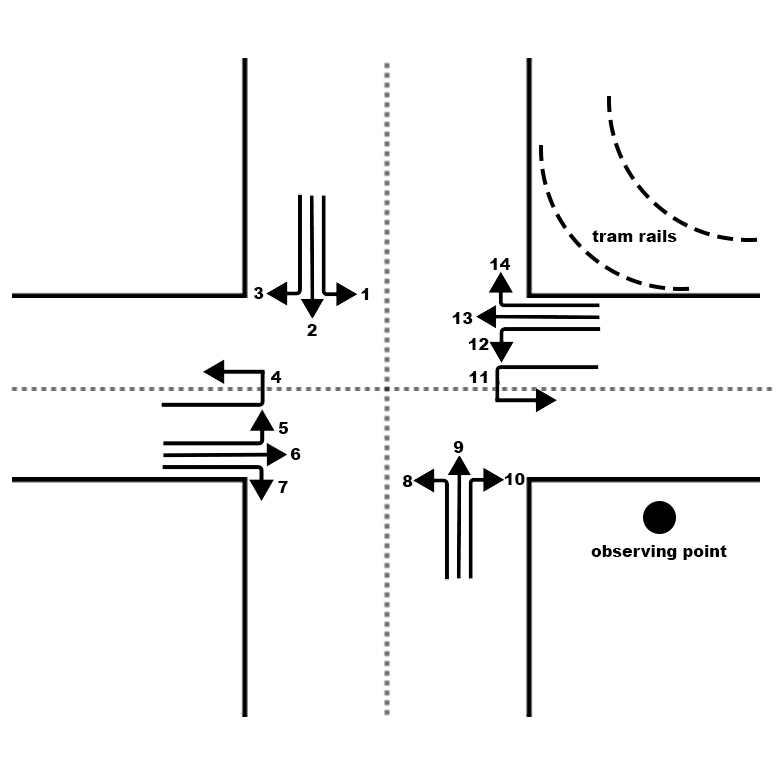
\includegraphics[width=.9\linewidth]{intersection.jpg}
\caption{Sketch of the intersection Universitätsallee and Otto-Hahn-Allee in Bremen, Germany}
\label{fig:intersection}
\end{figure}

A total of four separate experiments were conducted, with each experiment containing four individual measurements for a time period of 10 minutes. The date, time, and temperature of each experiment is shown in Table \ref{tbl:experiments}. Starting at the predetermined time, a stop watch was started for exactly 10 minutes. After a 5 minute break, another measurement was conducted identically.
\begin{center}
\begin{tabular}{ |p{4.5em}|p{3.5em}|p{7.5em}|p{5.5em}|}
 \hline
 Experiment & Date & Time & Temperature  \\
 \hline
 1 & 30.05.22 & 8:05am - 9:00am & $9^\circ$C - $10^\circ$C \\
 \hline
 2 & 30.05.22 & 9:05am - 10:00am & $11^\circ$C \\
 \hline
  3 & 03.06.22 & 9:05am - 10:00am & $14^\circ$C - $17^\circ$C\\
 \hline
  4 & 10.06.22 & 9:05am - 10:00am & $18^\circ$C - $19^\circ$C \\
 \hline
\end{tabular}
\captionof{table}{Dates, times, and temperatures of each experiment}
\label{tbl:experiments}
\end{center}
~\\
During each measurement the amount of cars taking a certain path and their according timestamp, in minutes and seconds (e.g. 1:21) was noted. Vehicles such as trams, buses and motorcycles were marked separately. Generally, the timestamp was noted when a vehicle crossed the center of the intersection. 
In case that multiple cars take the same path at the same time the number of cars was noted next to the timestamp. This was done on provided data sheets. The data sheets are shown in the appendix. They contain the date, starting time, group number and temperature for each individual 10-minute-measurement in the top left corner.



\section{Data records}
\label{sec:Data_records}
Digital scans of the original data sheets containing the raw vehicle data are attached in the appendix. Furthermore, it was digitized into a Google-Spreadsheet-Dataset \cite{dataset_google_sheets}, specifically in the sub-spreadsheet "Group 1". The spreadsheet with some evalutations of the data shown in Section \ref{sec:Technical_validation} as well as the Latex files for this paper and scans of the original data sheets are also available on GitHub \cite{github}.

The data set is composed of four different sections for each experiment with each section containing four tables of all measurements. The amount of vehicles for each minute is summed up. Therefore, the seconds are not represented in the Google data set. For instance, if the timestamps for two cars are 0:12 and 0:59, they would both count for the first minute of the experiment in the table. The timestamps are listed in the far left column. 

If cars, buses, motorcycles or trams simultaneously took the same path during the same minute, the sum of all vehicles was noted and the number of buses/motorcycles/trams was specified in brackets. For example, if four cars and a bus took the same path within the same minute, it would be noted as "5 (1 Bus)" in the table. A snippet of a Google table is presented in Figure \ref{fig:google_table_screenshot}, which shows the experiment section, timestamp and direction columns, as well as the latter example.

~\\
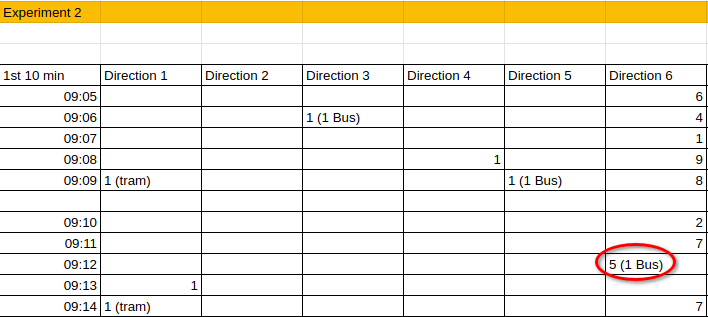
\includegraphics[width=0.95\linewidth]{Screenshot_20220613_112904.png}
\captionof{figure}{Snippet of Google spreadsheet table for Experiment 2}
\label{fig:google_table_screenshot}

\section{Technical validation}
\label{sec:Technical_validation}

This section provides the technical validation of the gathered data.
Overall 2331 vehicles were counted in all four experiments. Most of them drove straight on Universitätsallee (direction 6 and direction 13), which has two lanes in each direction. As shown in Figure \ref{fig:direction_pie} $49.46\%$ drove from the Autobahn into Bremen and $36.14\%$ from Bremen towards the Autobahn. It is also noticable, that not a single vehicle traveled from Otto-Hahn-Allee to Bibliotheksstraße (direction 9).
\begin{figure}[htbp]
\begin{center}
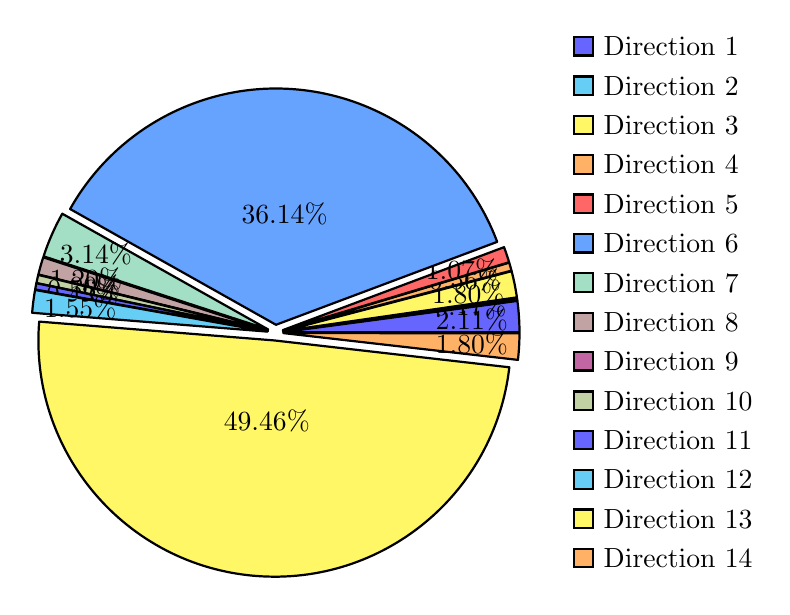
\begin{tikzpicture}
\pie[explode = 0.1, text = legend]{
    2.11/Direction 1,
    0.17/Direction 2,	
    1.80/Direction 3, 
    0.56/Direction 4, 
    1.07/Direction 5, 
    36.14/Direction 6, 
    3.14/Direction 7, 
    1.20/Direction 8, 
    0.00/Direction 9, 
    0.56/Direction 10, 
    0.43/Direction 11, 
    1.55/Direction 12,	
    49.46/Direction 13, 
    1.80/Direction 14}
\end{tikzpicture}
%\captionof{figure}{Proportion of vehicles driving in each direction}
\caption{Proportion of vehicles driving in each direction}
\label{fig:direction_pie}
\end{center}
\end{figure}
Out of the 2327 vehicles $2.32\%$ were buses and $1.89\%$ were trams as shown in Table \ref{tbl:no_vehicles}. Only six motorcycles were counted, since in high traffic sometimes motorcycles were not separately marked. Cars and trucks were counted as private vehicles, which made up $95.53\%$ of all vehicles.\\

\begin{tabular}{ |p{4em}|p{3em}|p{3em}|p{3em}|p{5em}|}
 \hline
 & Private & Buses & Trams & Motorcycles\\
 \hline
 Absolute & 2223 & 54 & 44 & 6\\
 \hline
 Percentage & 95.53\% & 2.32\% & 1.89\% & 0.26\% \\
 \hline
\end{tabular}
\captionof{table}{Number and percentage of each vehicle type across all experiments}
\label{tbl:no_vehicles}
~\\
Figure \ref{fig:vehicle_types} shows the number of each vehicle types in each experiment. Experiments 3 and 4 which were both conducted on a Friday at the same time show similar numbers of private vehicles, buses and Trams. Also experiment 2 has comparable numbers of private vehicles and buses and only a slightly higher number of trams. Only experiment 1 sees much higher numbers of private vehicles, probably because it was conducted an hour earlier and therefore more people were on their way to work.\\

\pgfplotstableread{Vehicle_Numbers.txt}{\table}
\begin{tikzpicture}
%\begin{axis}[xtick distance = 1]
\begin{semilogyaxis}[
    group style={
        %group name=my plots,
        %group size=1 by 2,
        xlabels at=edge bottom,
        xticklabels at=edge bottom,
        vertical sep=0pt},
        width = \linewidth,
        %axis lines = middle,
        xmin = 0.5, xmax = 4.5,
        legend style={at={(0.95,0.5)},anchor=south east},
        xlabel = {Experiment No.},
        ylabel = {Number of Vehicles}]
        %legend pos = center west]

\addplot[blue, only marks, mark = x] table [x = {x}, y = {Private}] {\table};
\addplot[red, only marks, mark = star] table [x = {x}, y = {Tram}] {\table};
\addplot[green, only marks, mark = +] table [x = {x}, y = {Bus}] {\table};
\addplot[orange, only marks, mark = triangle] table [x = {x}, y = {Motorcycle}] {\table};

\legend{Private,Tram, Bus, Motorcycle}
\end{semilogyaxis}
\end{tikzpicture}
\captionof{figure}{Number of different vehicle types in each of the four experiments}
\label{fig:vehicle_types}
~\\
Finally it is noteworthy that a lot of cars came in bulk, the main reason for this are either the traffic light on this intersection or traffic lights on previous intersections. This behavior cannot be observed using the digital data in the Google sheet, because it just describes the cars per minute, but in the physical data sheets in the appendix the accurate times are shown.
%%\newpage
\section{Appendix}
\subsection{Changes}
\begin{itemize}
    \item Changed former Background \& Summary to Introduction 
    \item Reworked and removed some parts of the text
    \item Added conclusion
    \item Added ''Bremen, Germany'' to Methods and intersection caption
    \item Moved date \& times from Technical Validation to Methods and added a table
    \item Increased size of intersection sketch 
    \item Improved axis scaling and labeling in Figure 4 
    \item Fixed spelling and grammar issues
    \item Thenuka indicated an error in the digitalization of our data, the data set was fixed and the data in the paper was adjusted accordingly
    \item Increased raw data sheet size in Appendix
    \item Uploaded the data to GitHub
    
\end{itemize}
\label{sec:Section 5}

\begin{figure*}[htbp]
  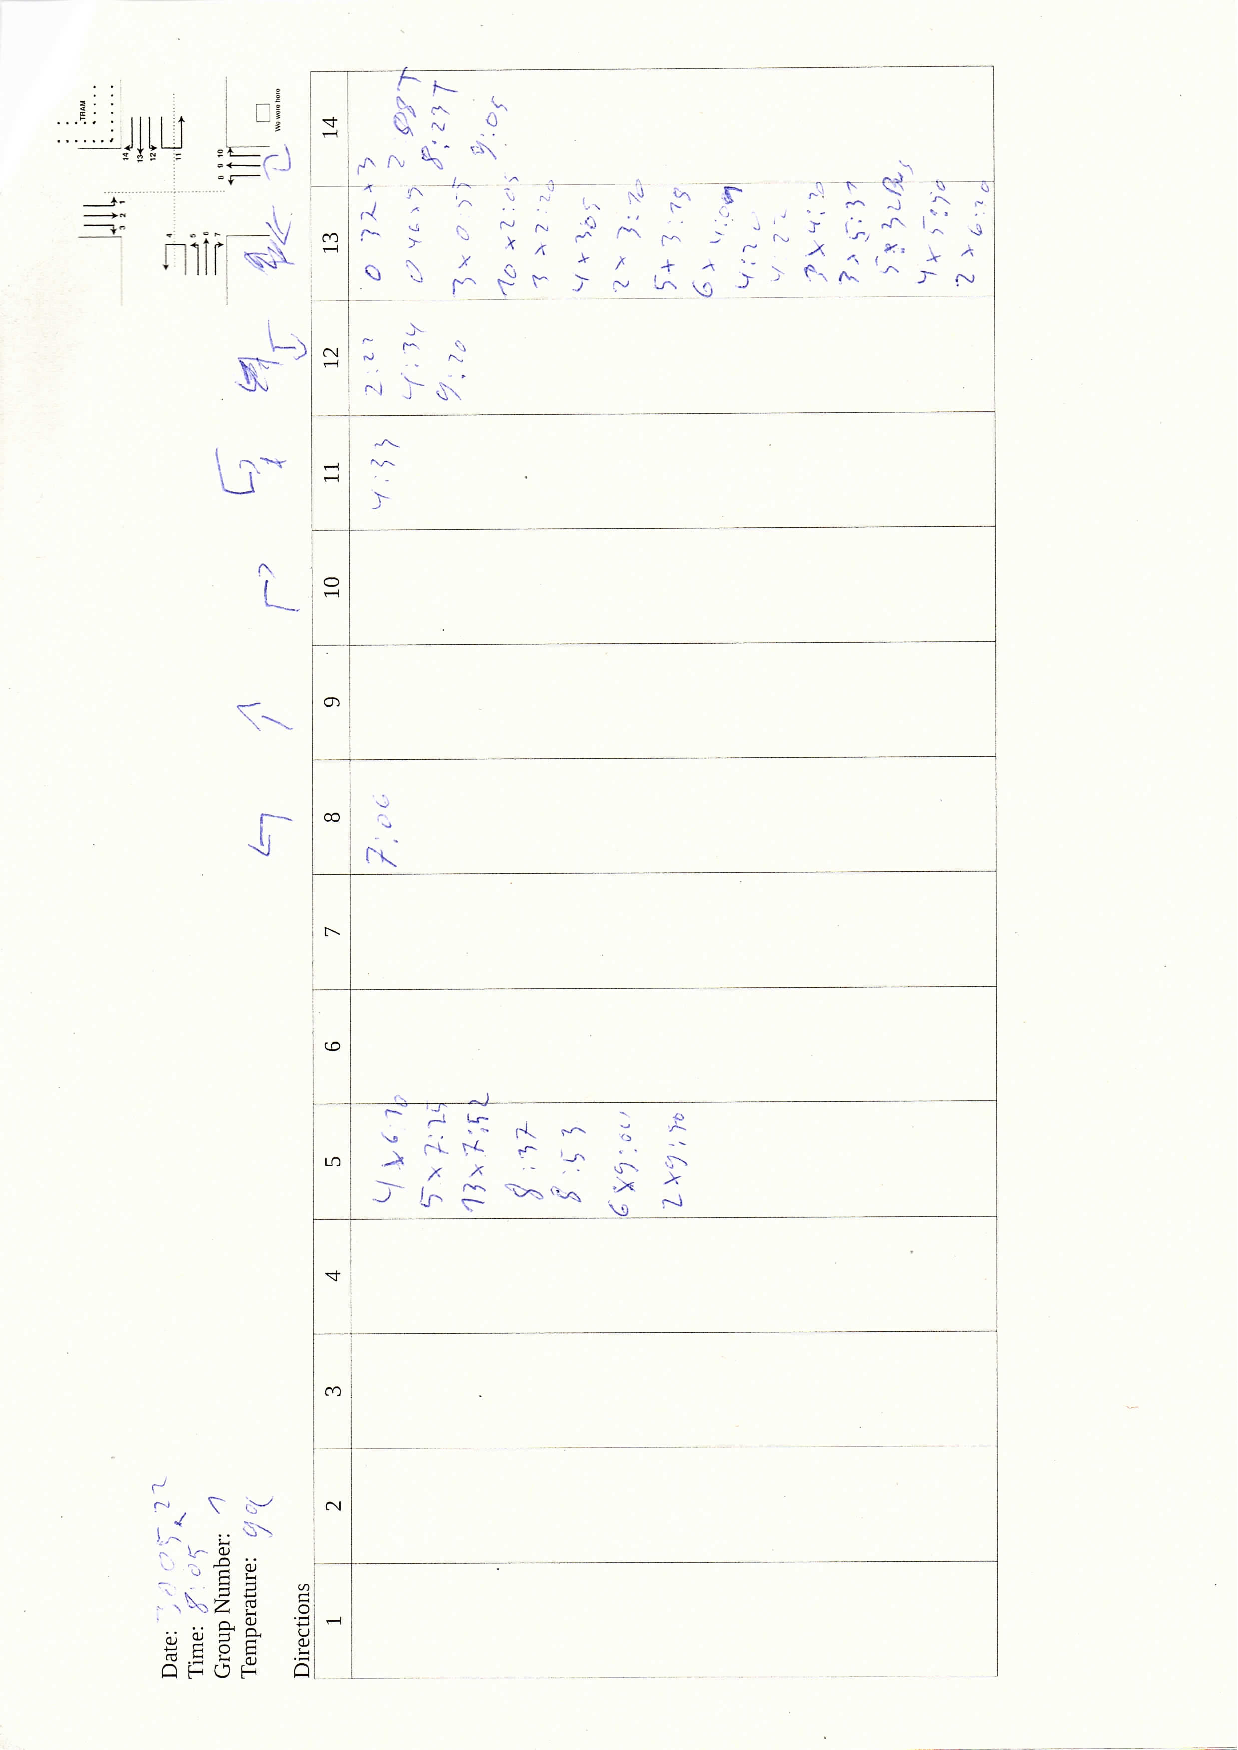
\includegraphics[width=\linewidth]{scans/300522_0805.pdf}
\end{figure*}

\begin{figure*}[htbp]
  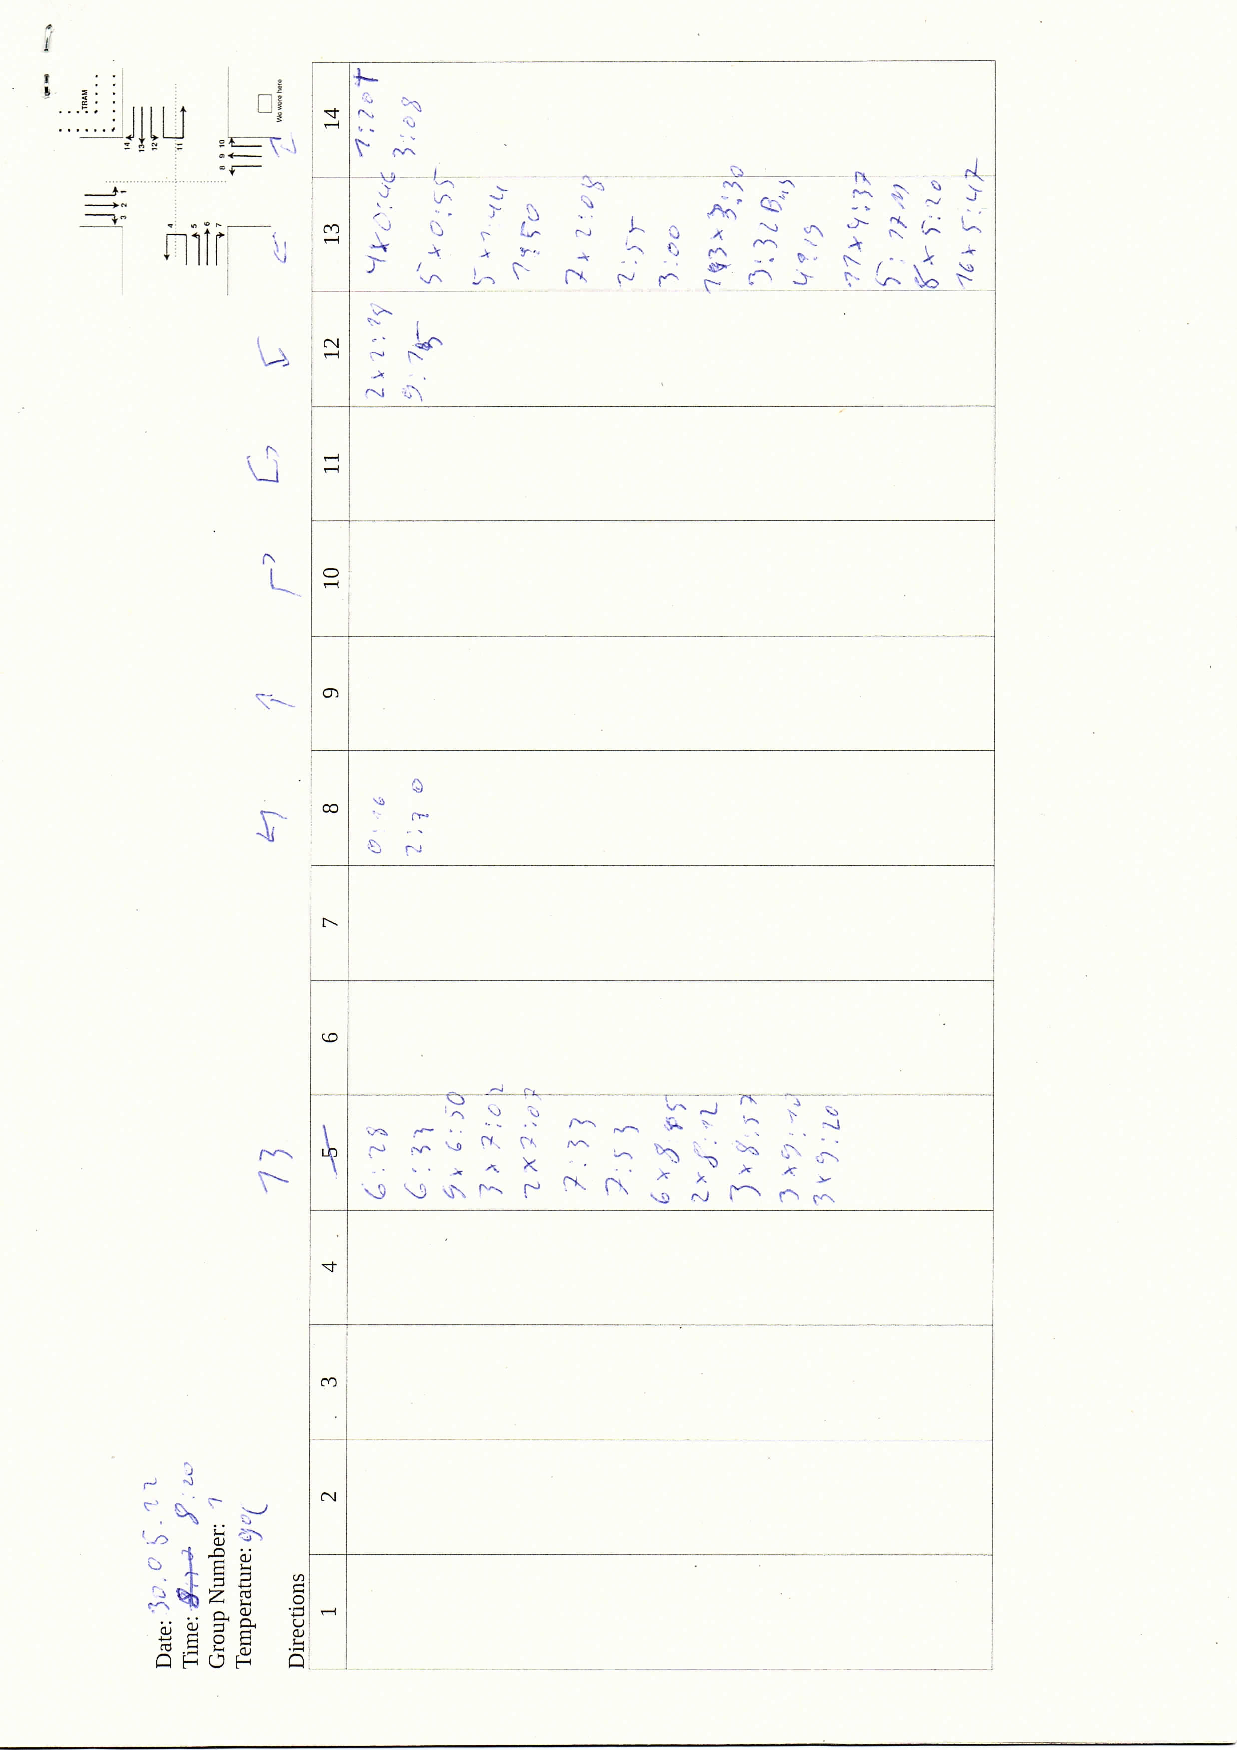
\includegraphics[width=\linewidth]{scans/300522_0820.pdf}
\end{figure*}

\begin{figure*}[htbp]
  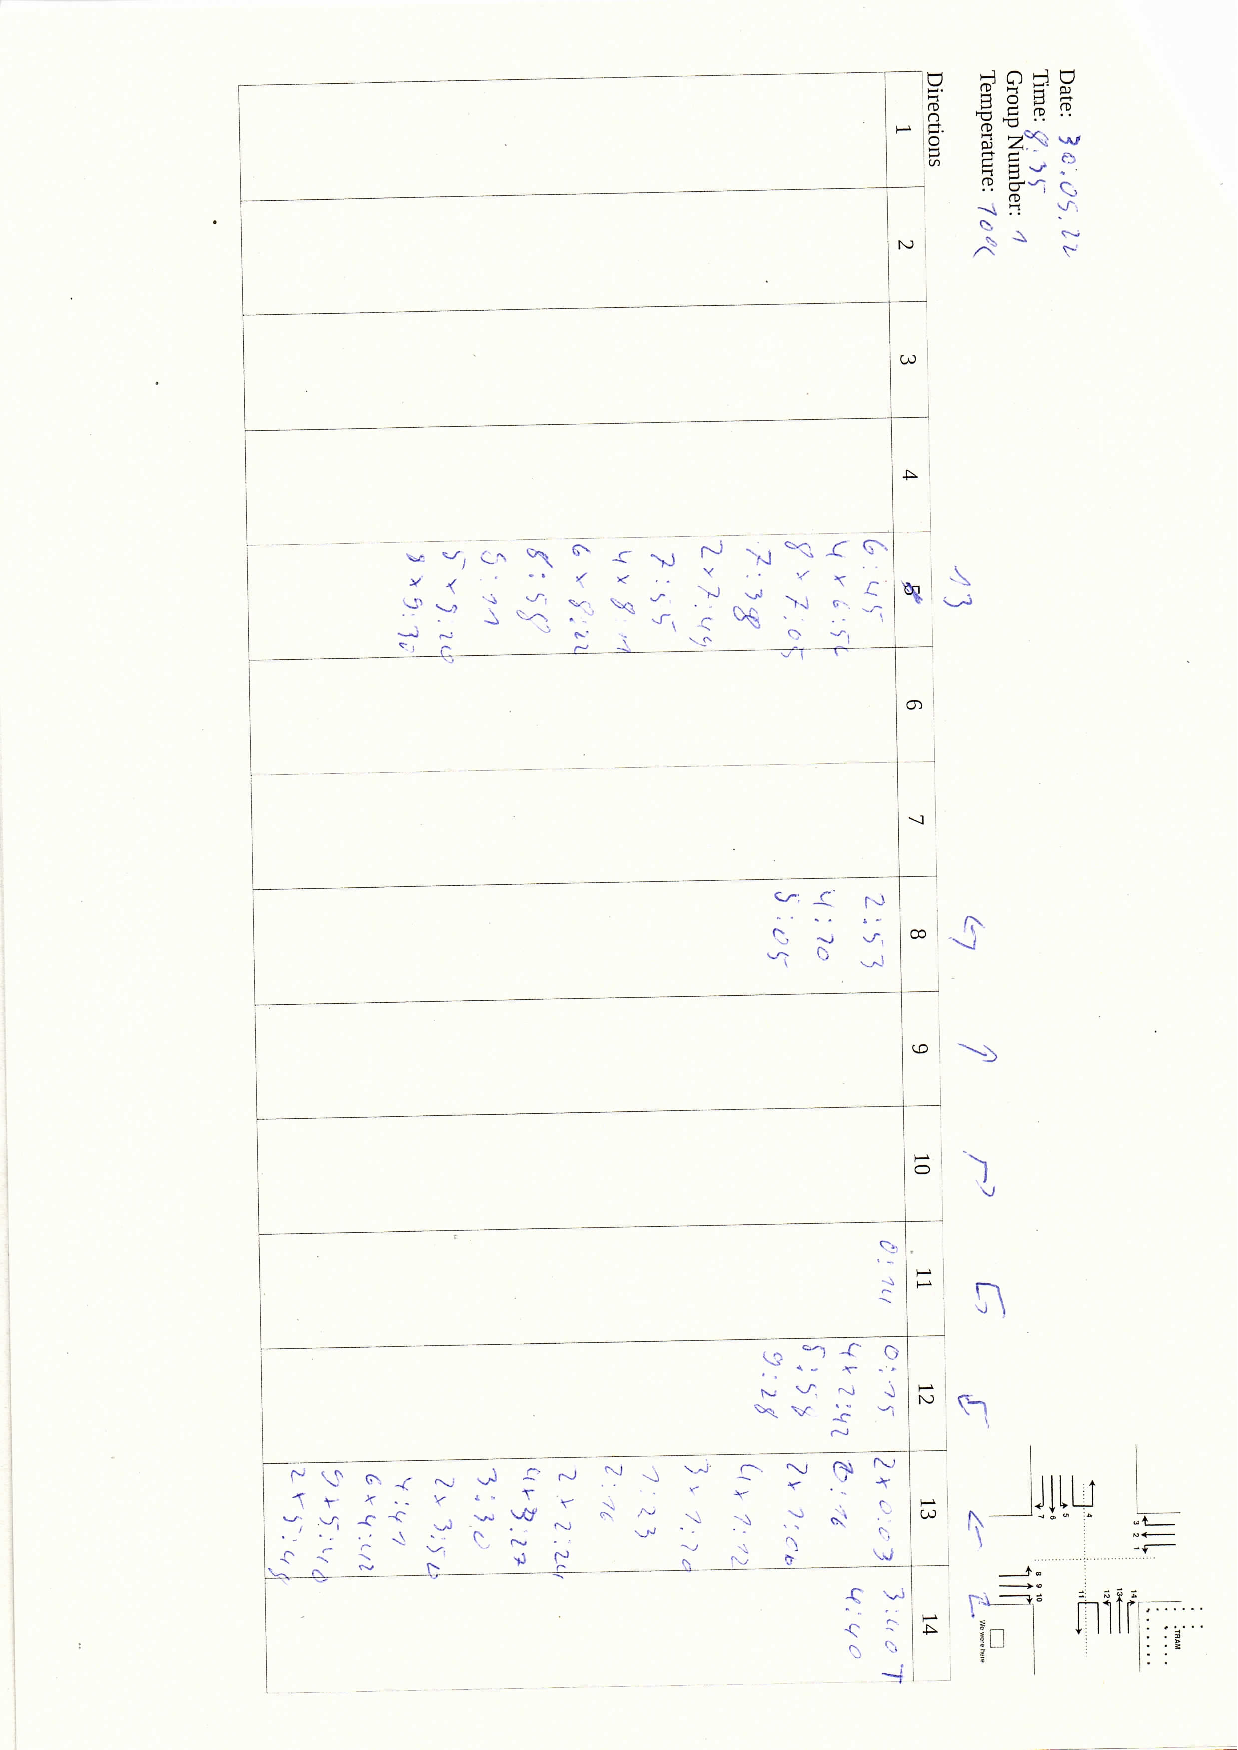
\includegraphics[width=\linewidth]{scans/300522_0835.pdf}
\end{figure*}

\begin{figure*}[htbp]
  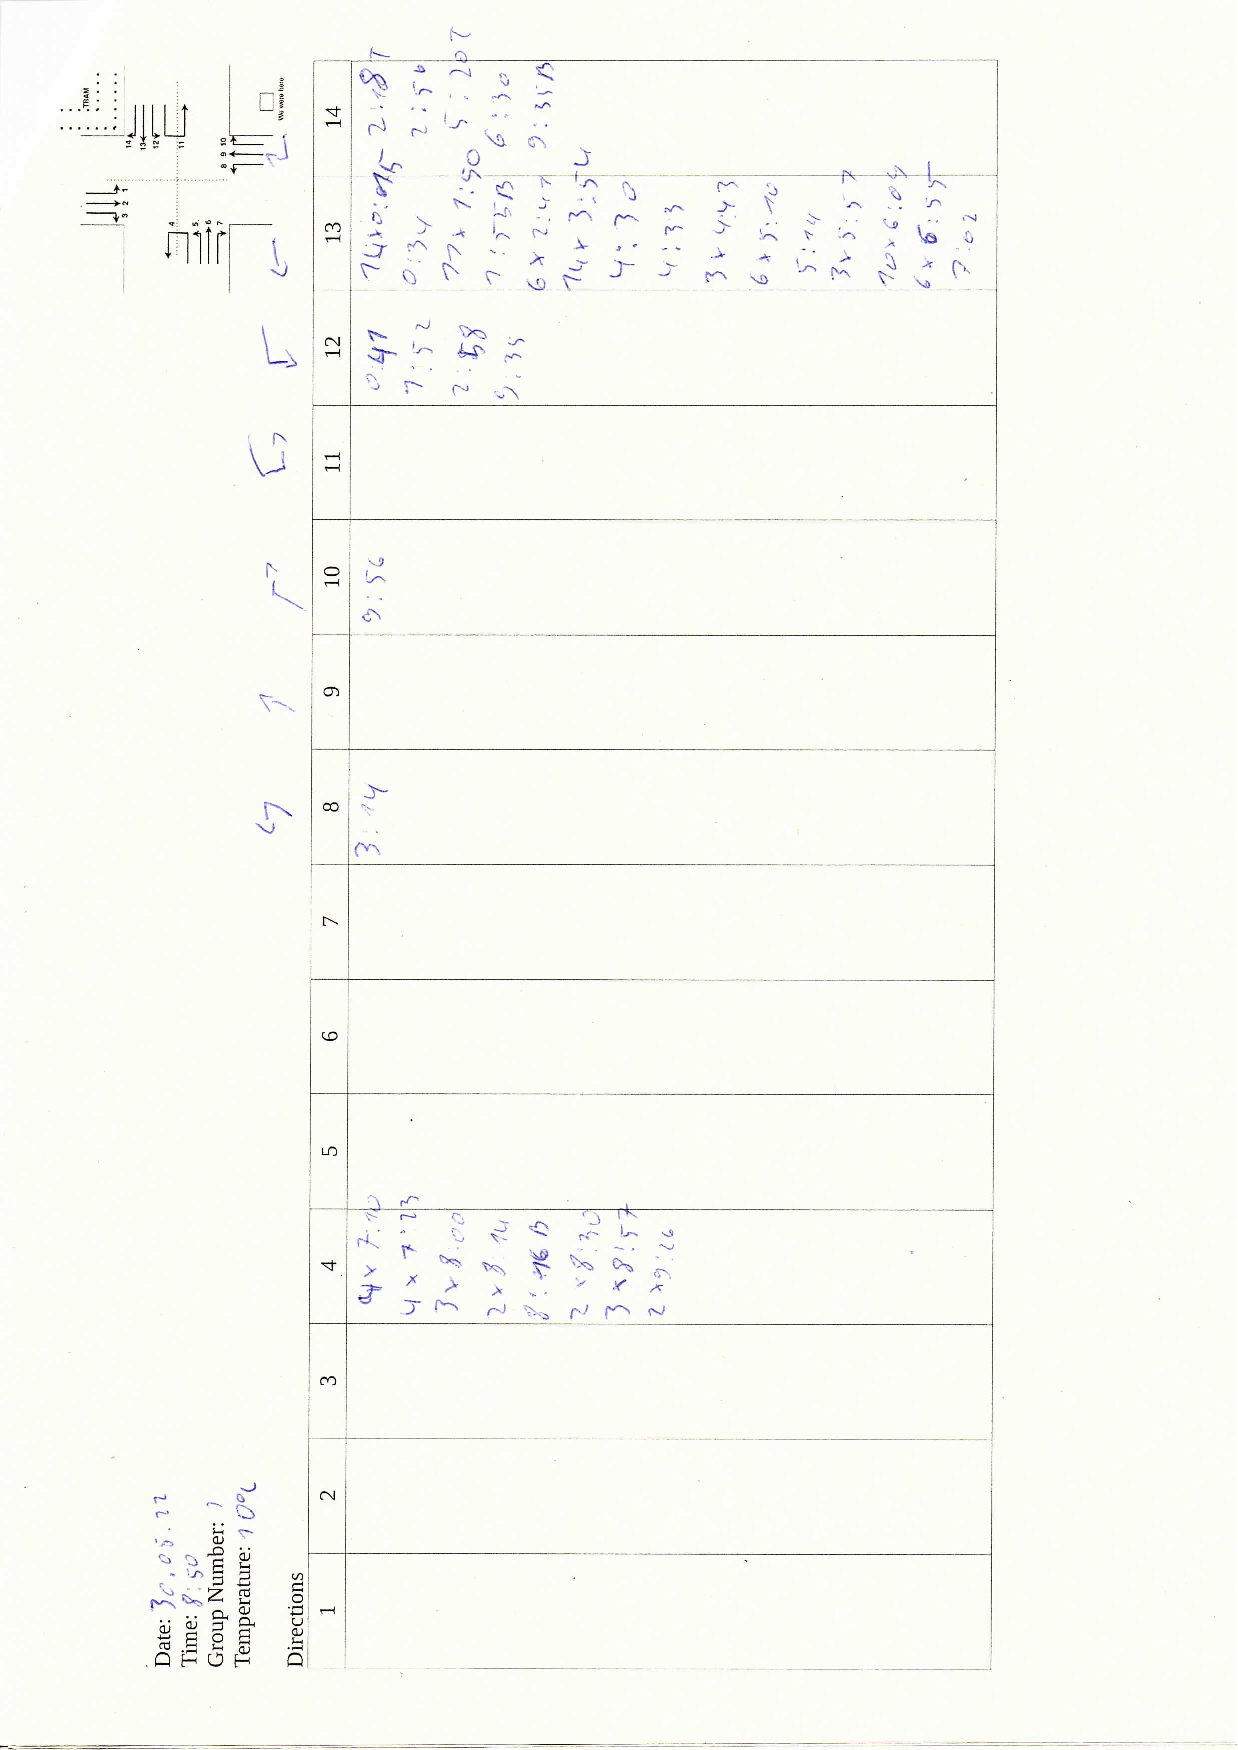
\includegraphics[width=\linewidth]{scans/300522_0850.pdf}
\end{figure*}


%\rotatebox{270}{\scalebox{.25}{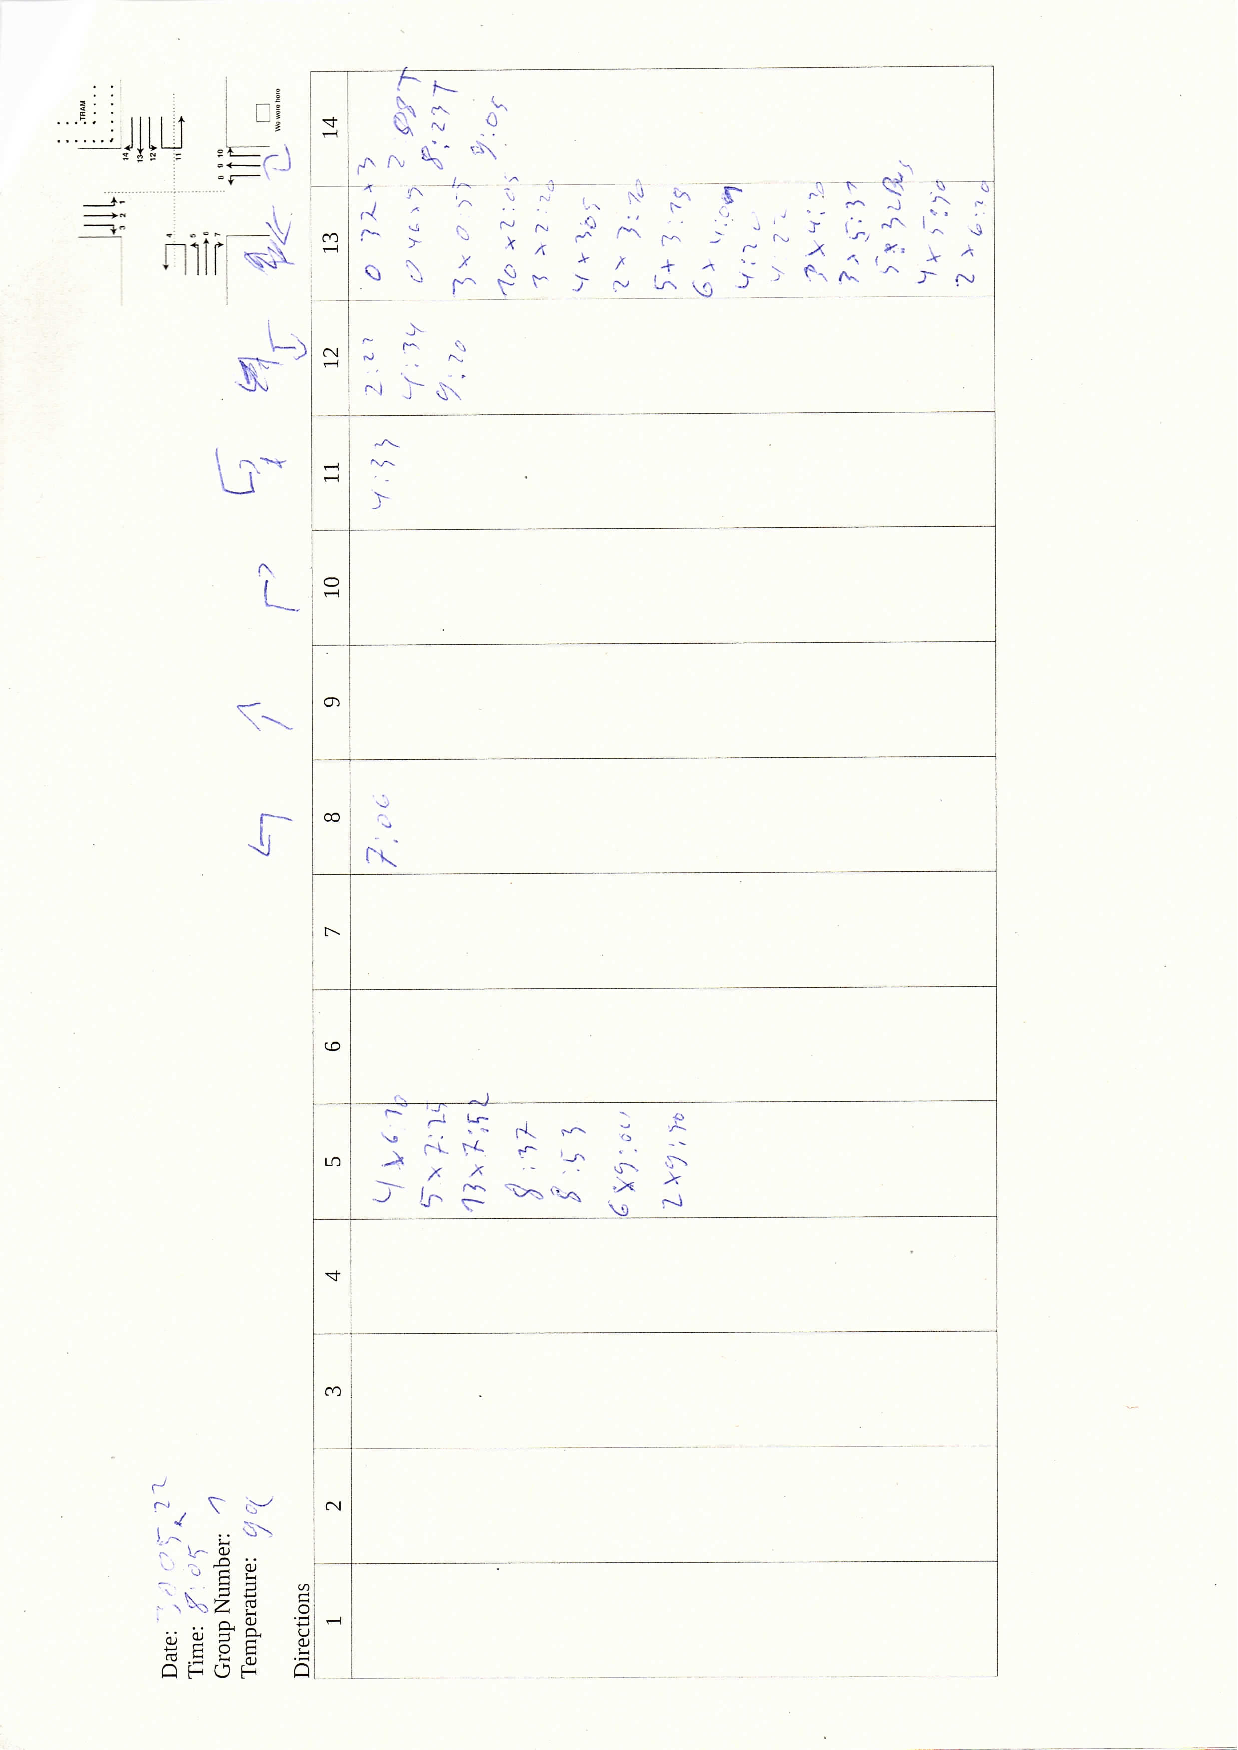
\includegraphics[]{scans/300522_0805.pdf}}}\\\\
%\rotatebox{270}{\scalebox{.25}{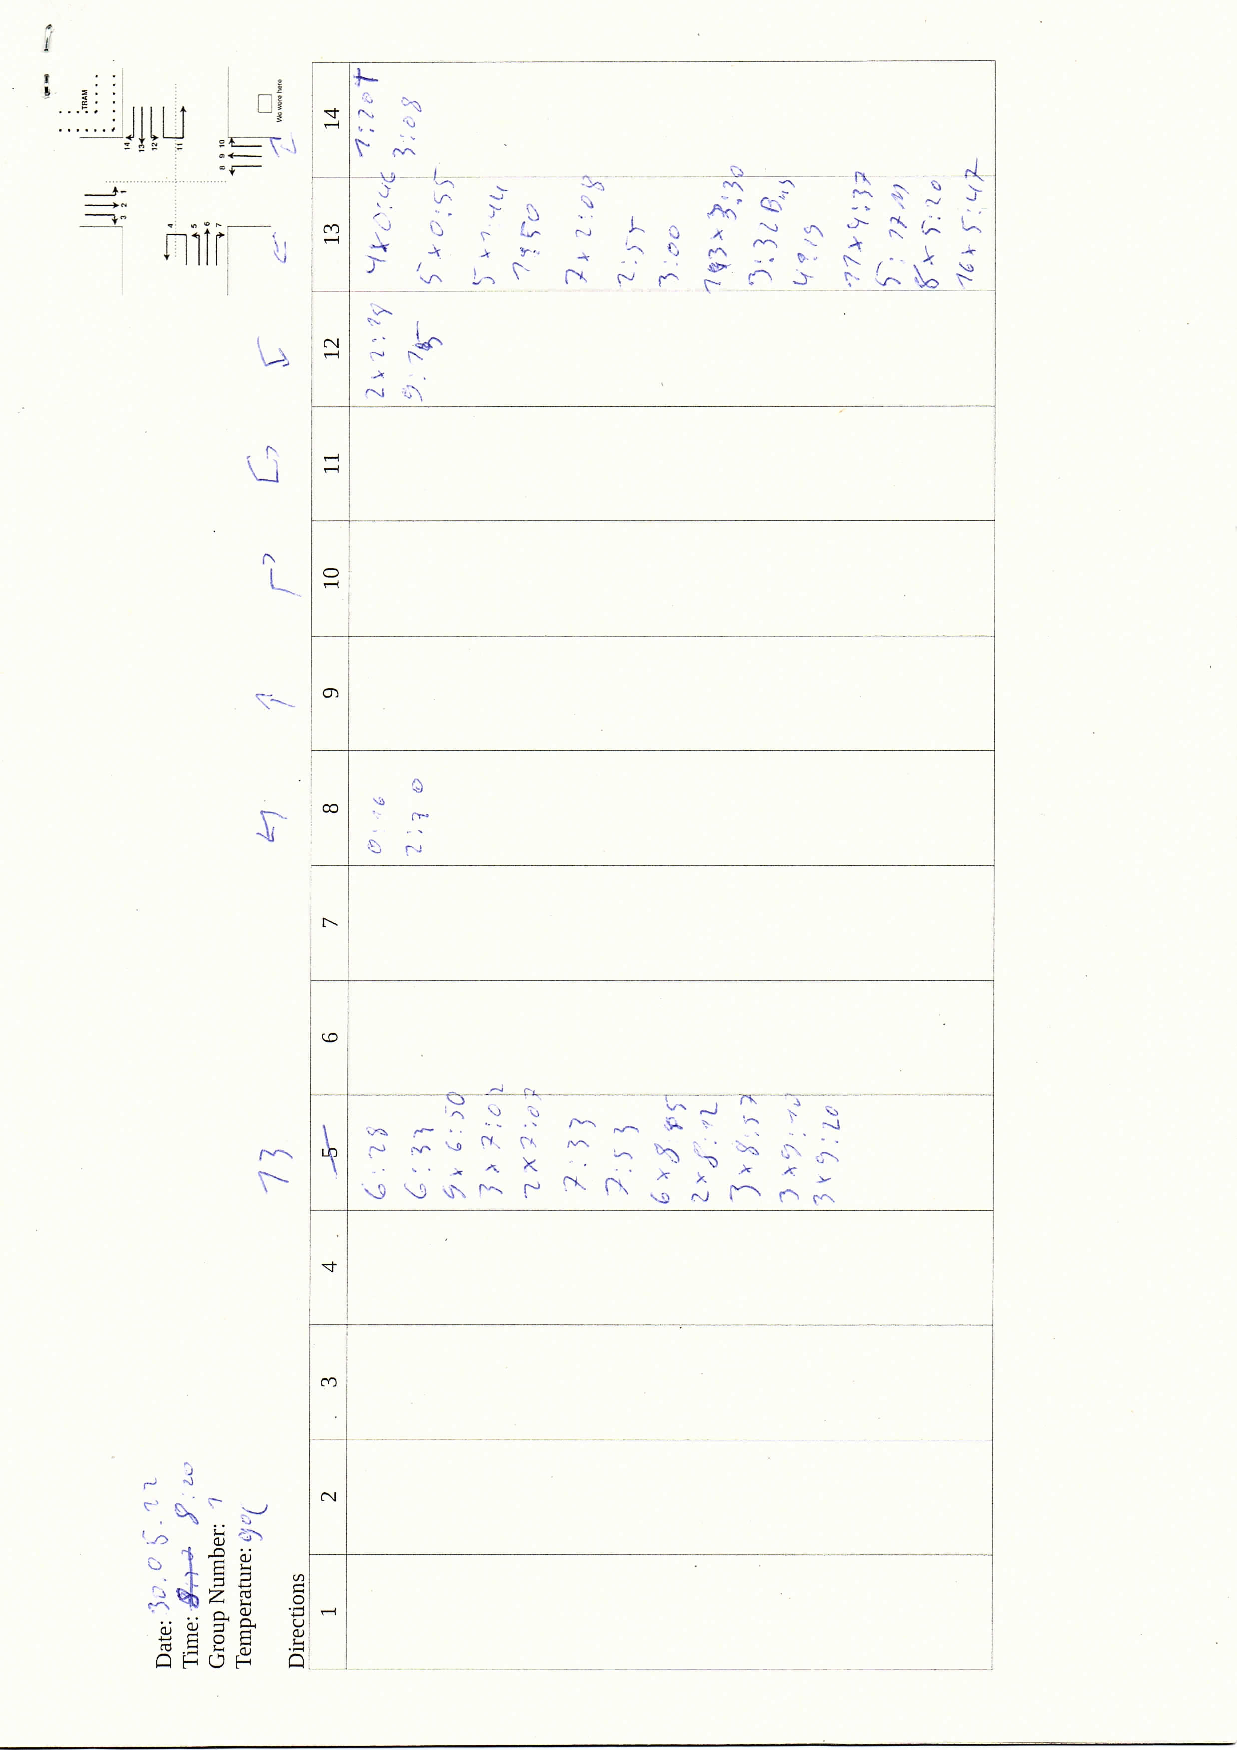
\includegraphics[]{scans/300522_0820.pdf}}}\\\\
%\rotatebox{90}{\scalebox{.25}{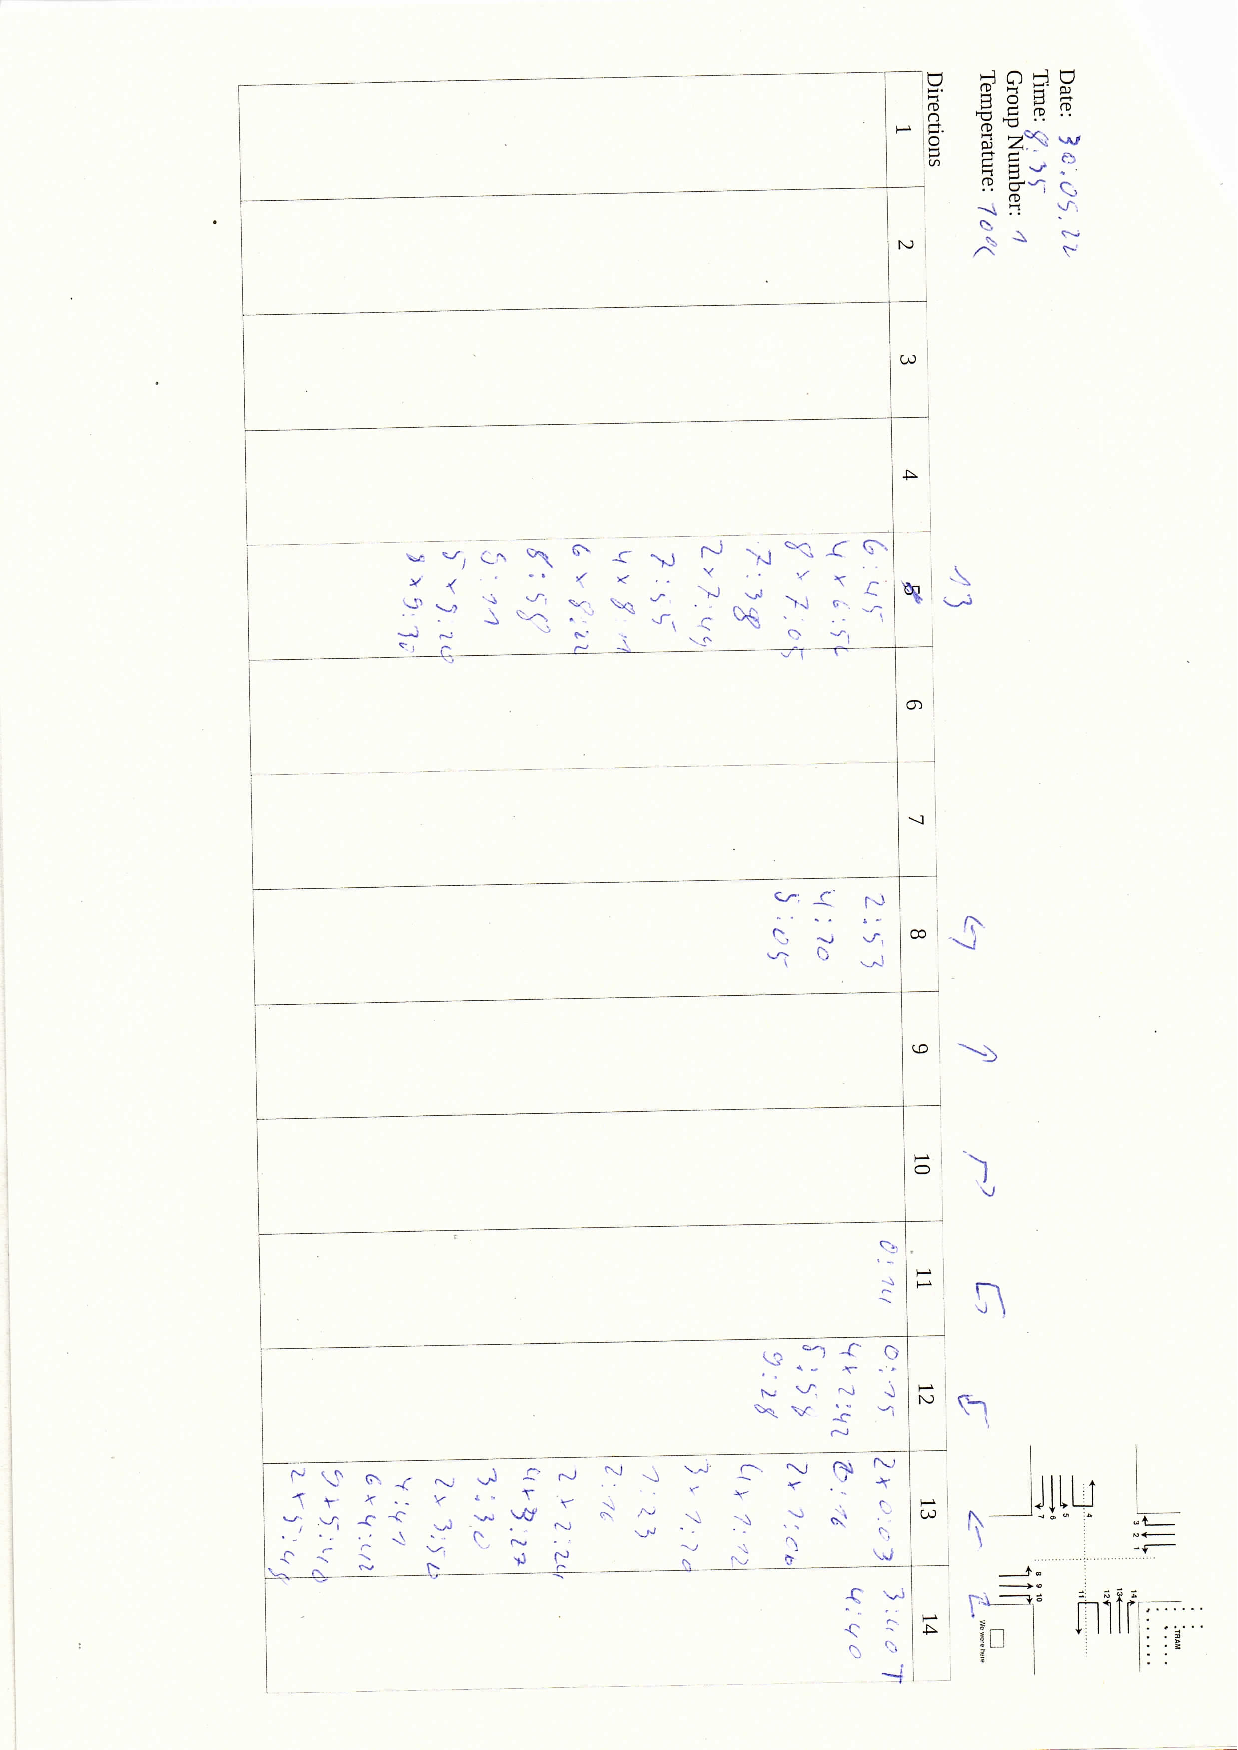
\includegraphics[]{scans/300522_0835.pdf}}}\\\\
%\rotatebox{270}{\scalebox{.25}{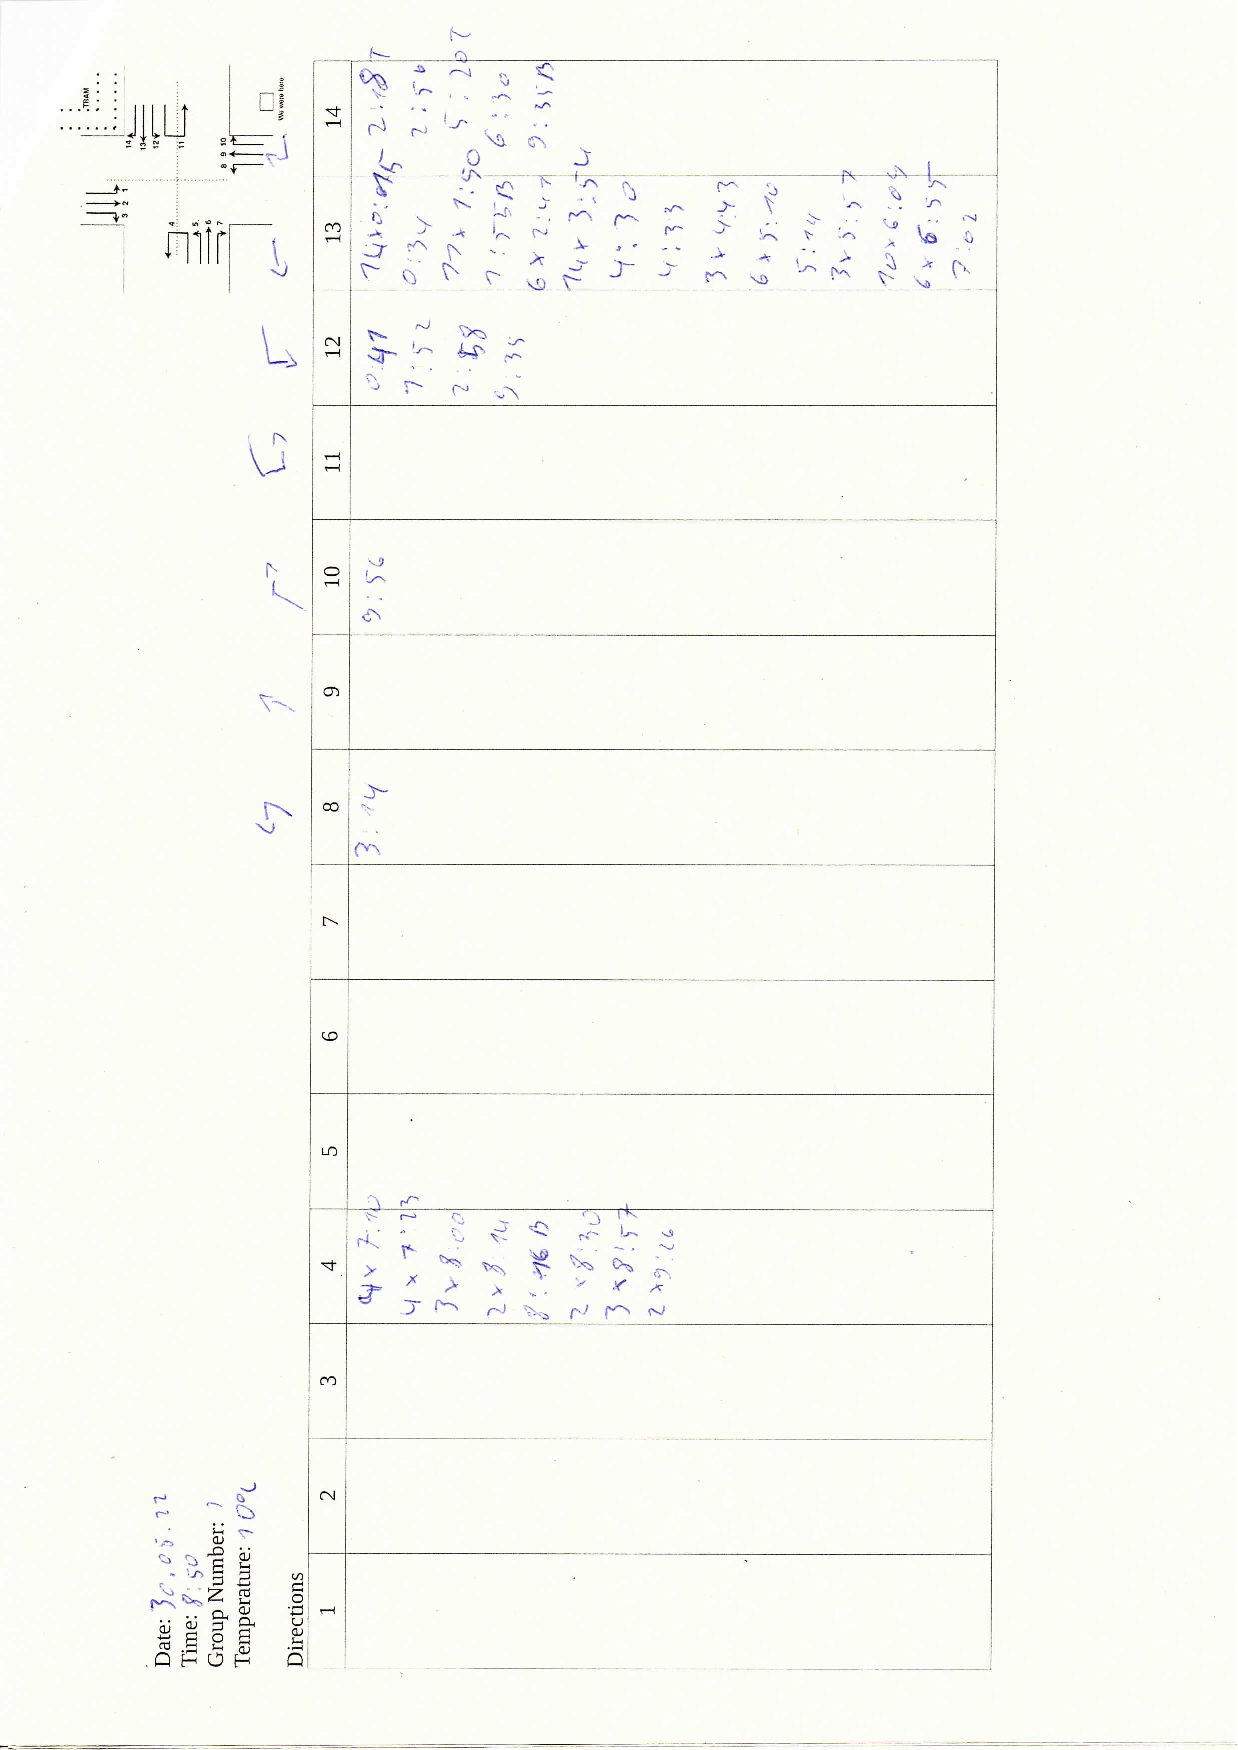
\includegraphics[]{scans/300522_0850.pdf}}}\\\\

\begin{figure*}[htbp]
  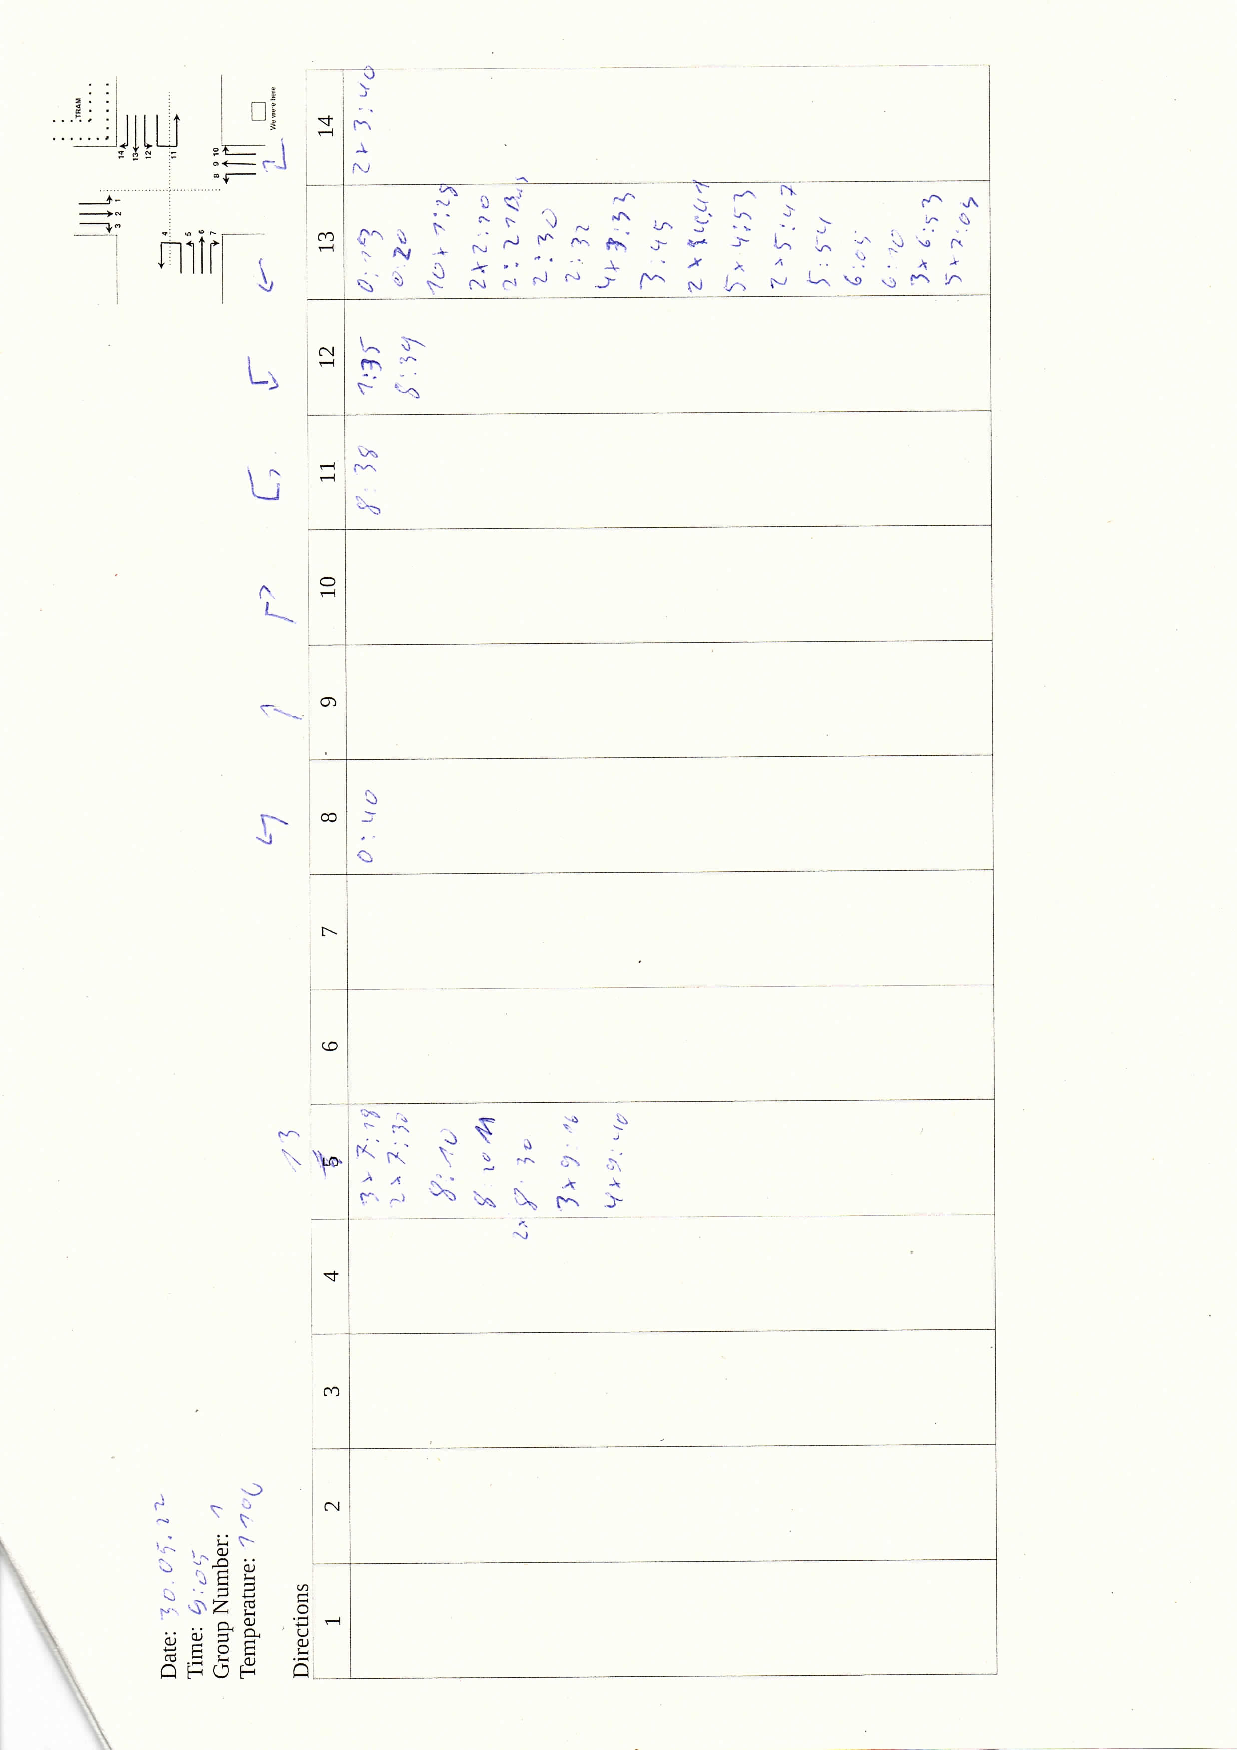
\includegraphics[width=\linewidth]{scans/300522_0905.pdf}
\end{figure*}

\begin{figure*}[htbp]
  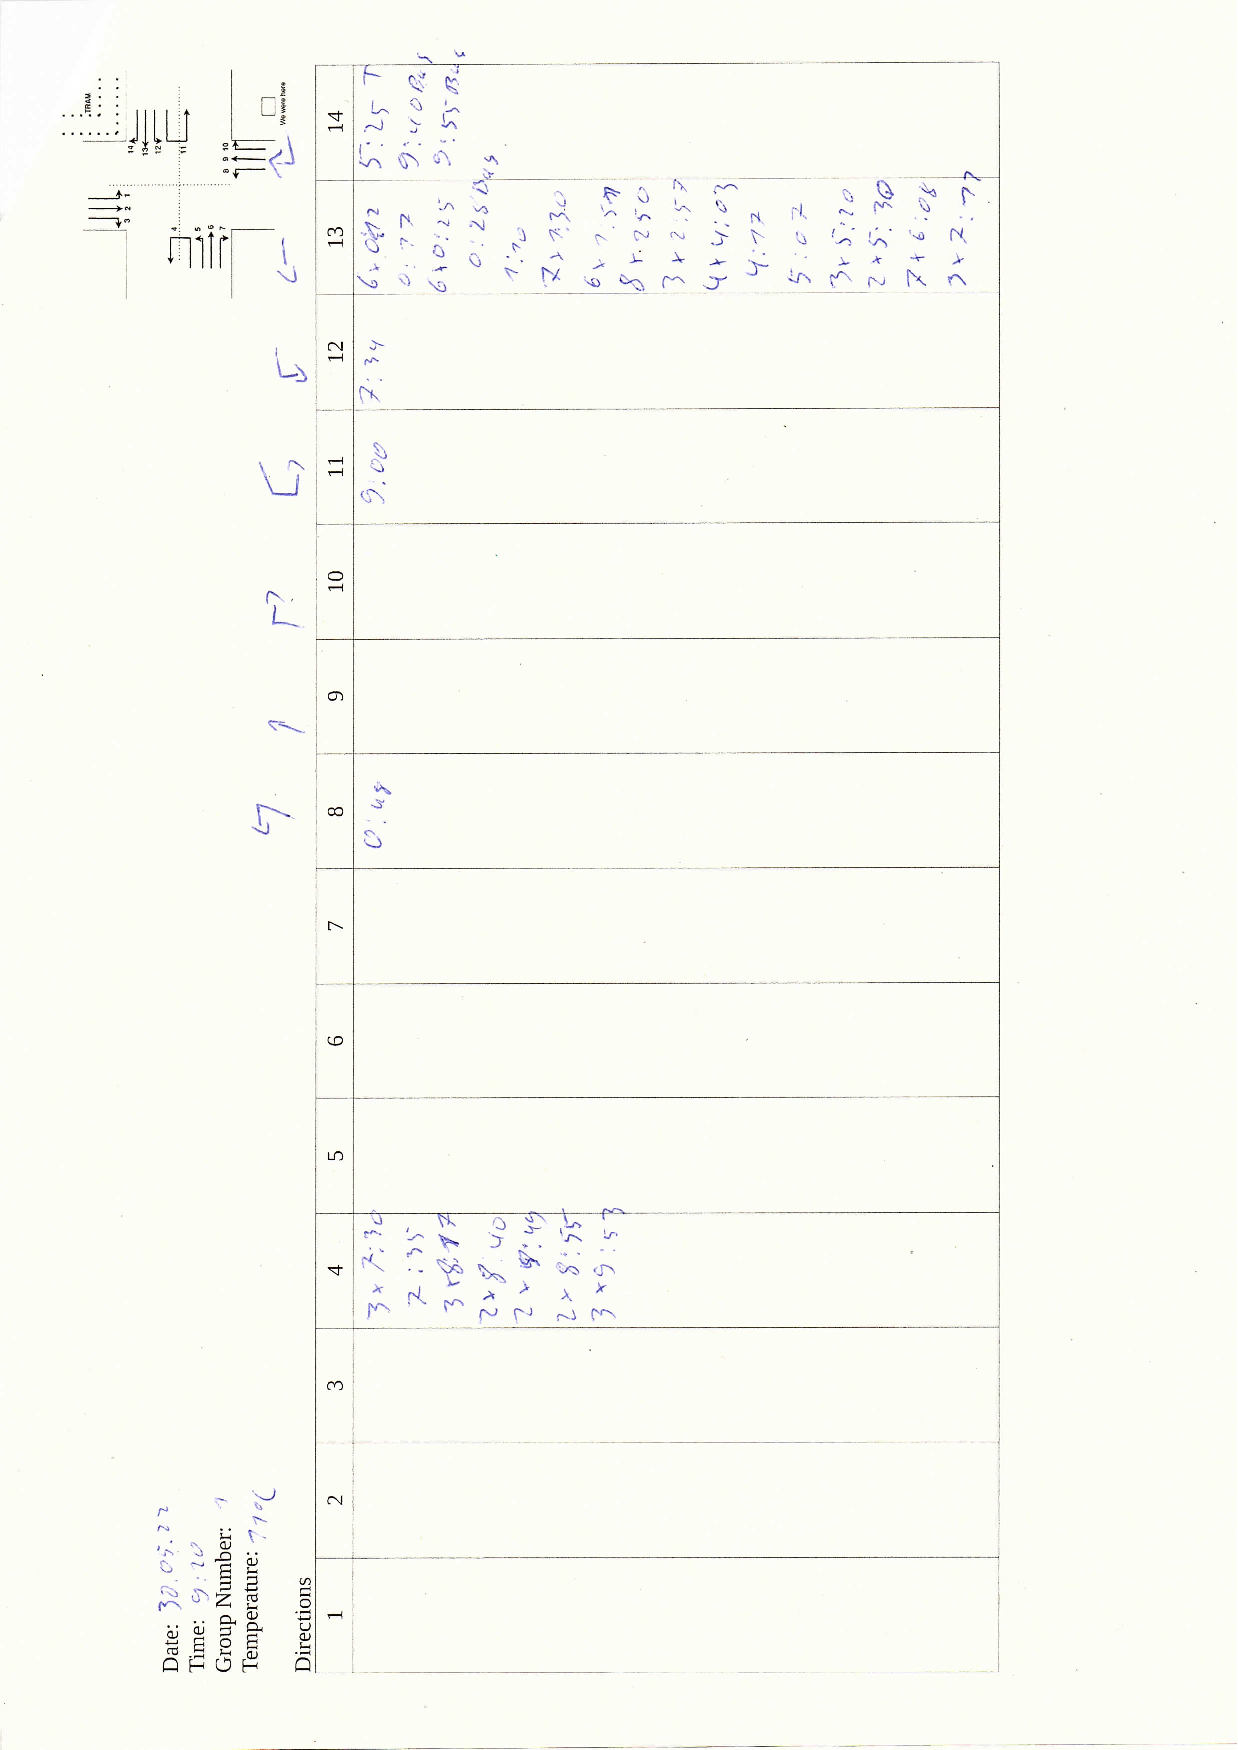
\includegraphics[width=\linewidth]{scans/300522_0920.pdf}
\end{figure*}

\begin{figure*}[htbp]
  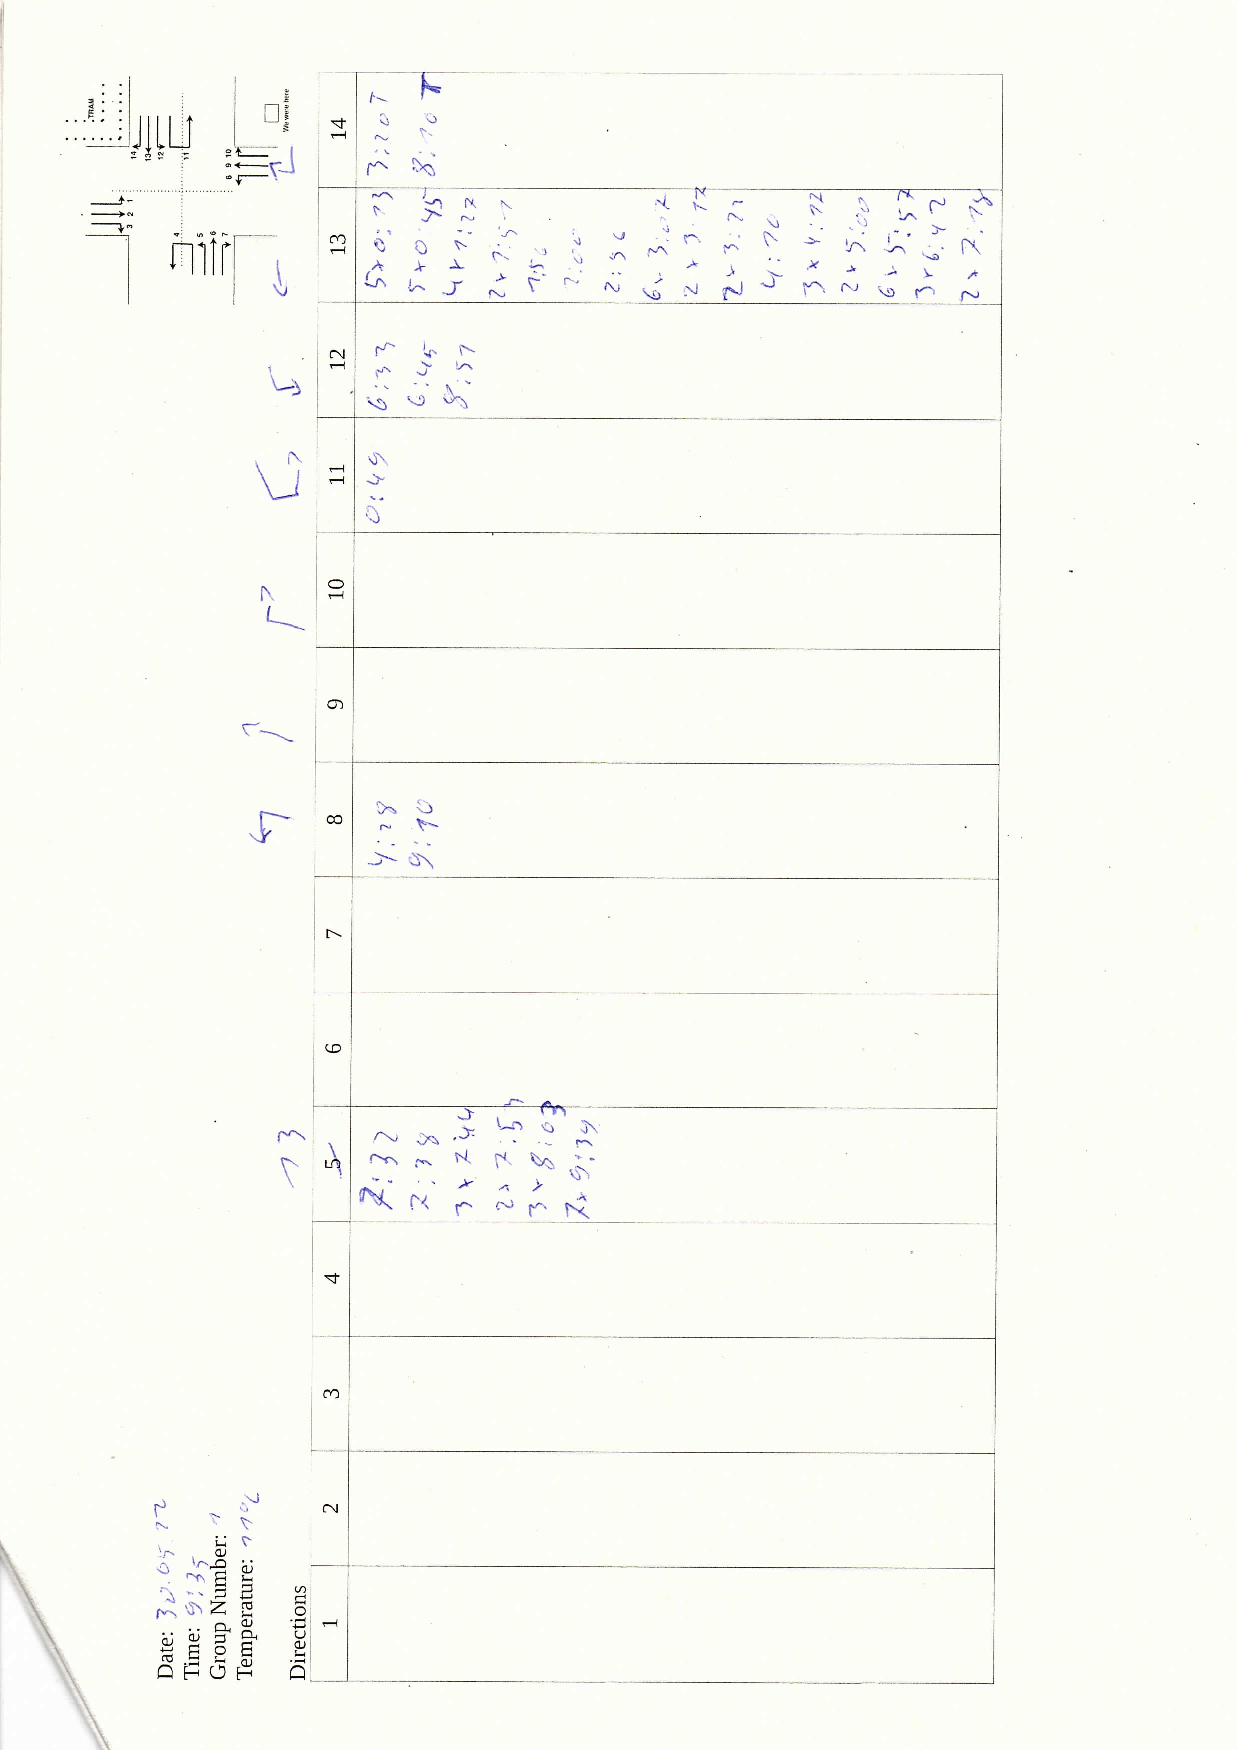
\includegraphics[width=\linewidth]{scans/300522_0935.pdf}
\end{figure*}

\begin{figure*}[htbp]
  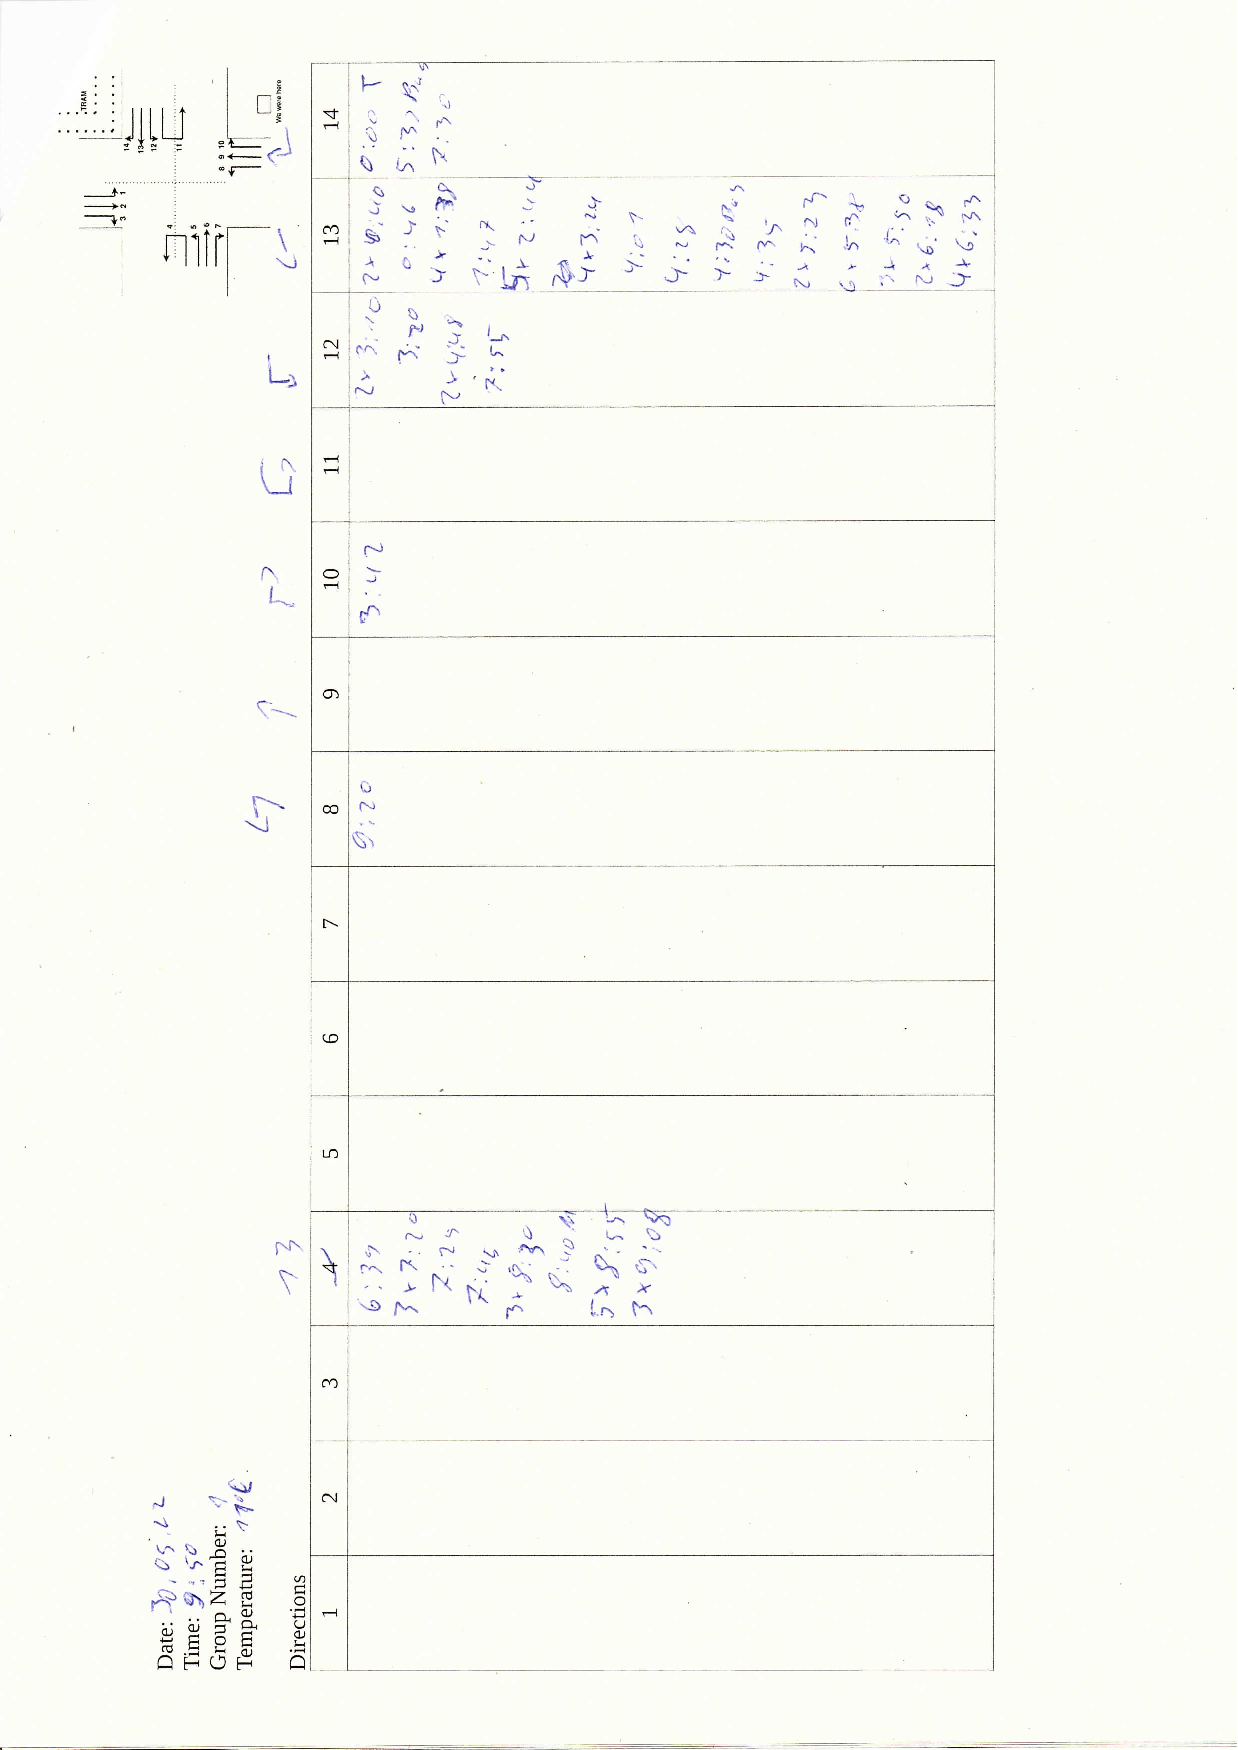
\includegraphics[width=\linewidth]{scans/300522_0950.pdf}
\end{figure*}

%\rotatebox{270}{\scalebox{.25}{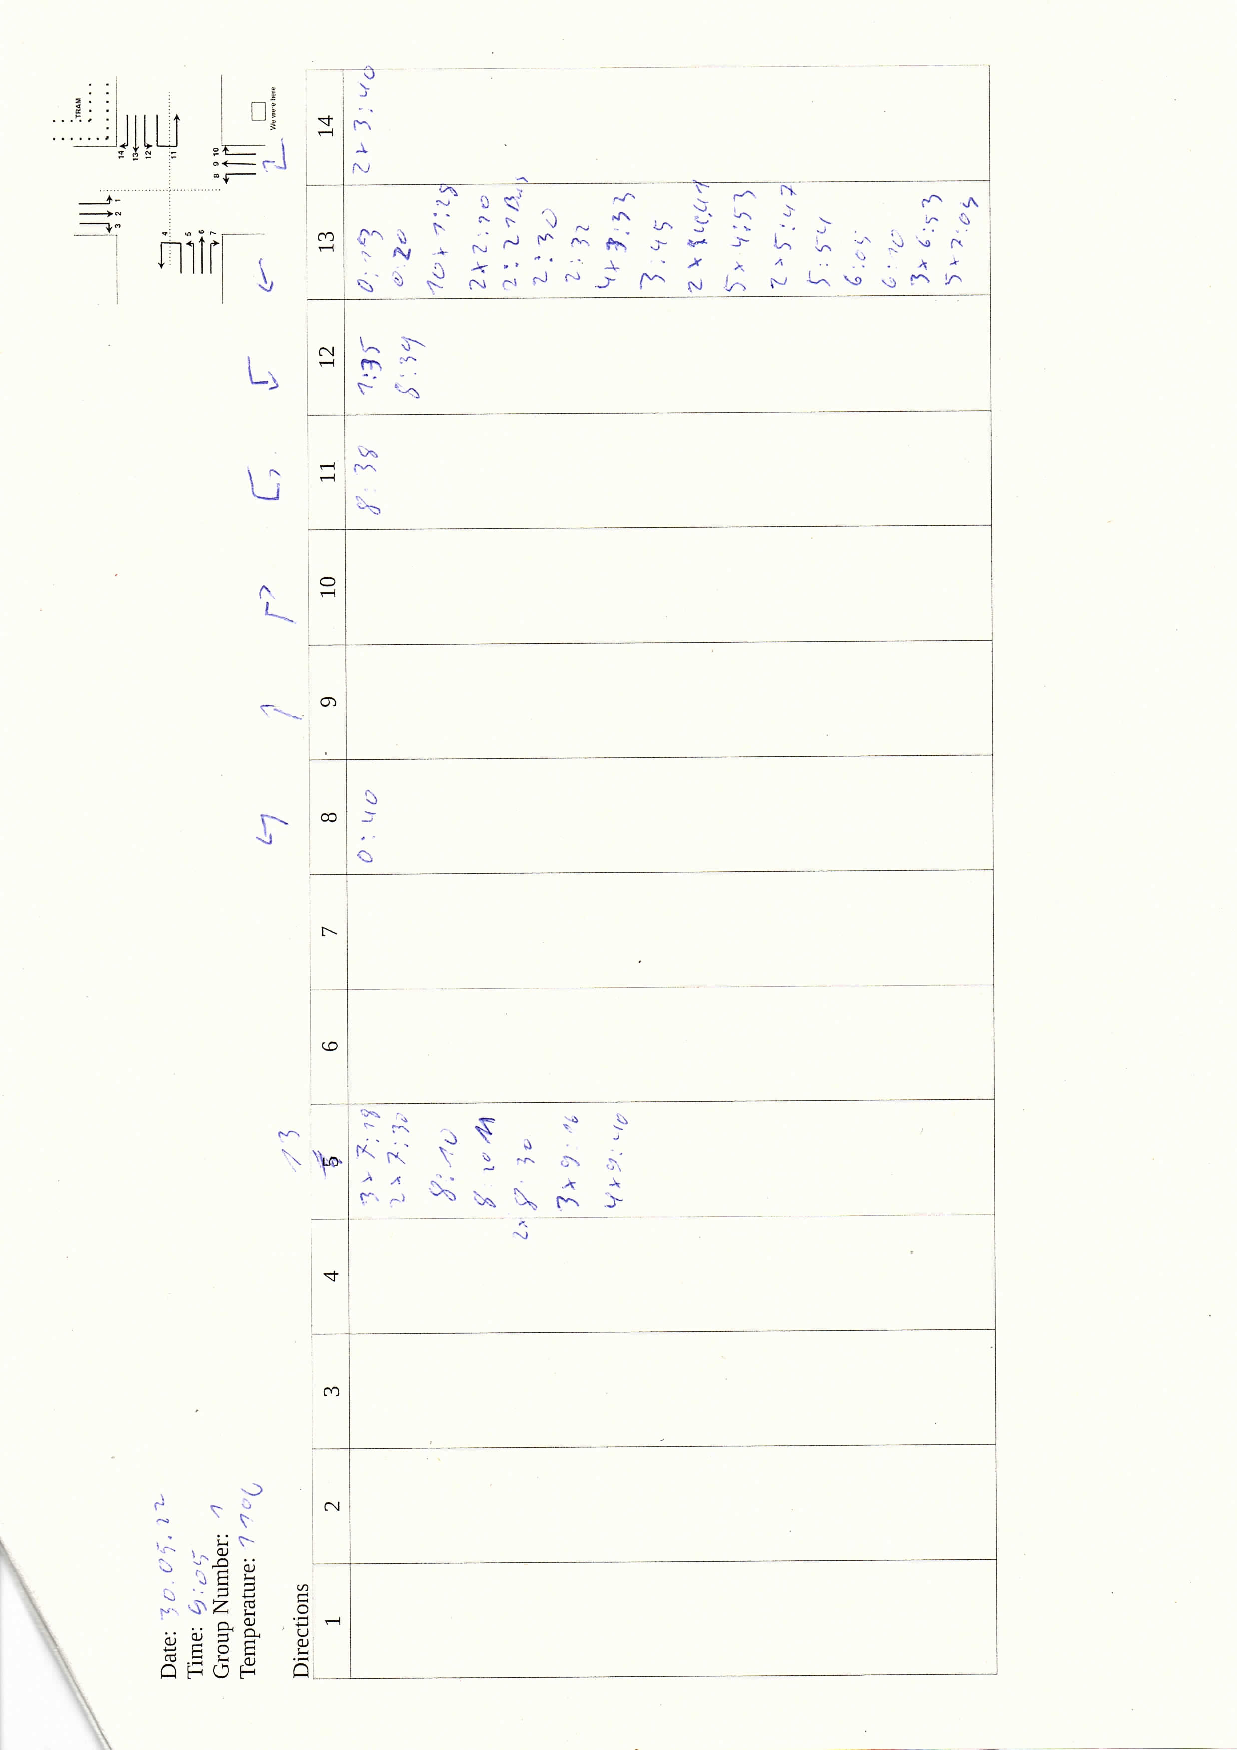
\includegraphics[]{scans/300522_0905.pdf}}}\\\\
%\rotatebox{270}{\scalebox{.25}{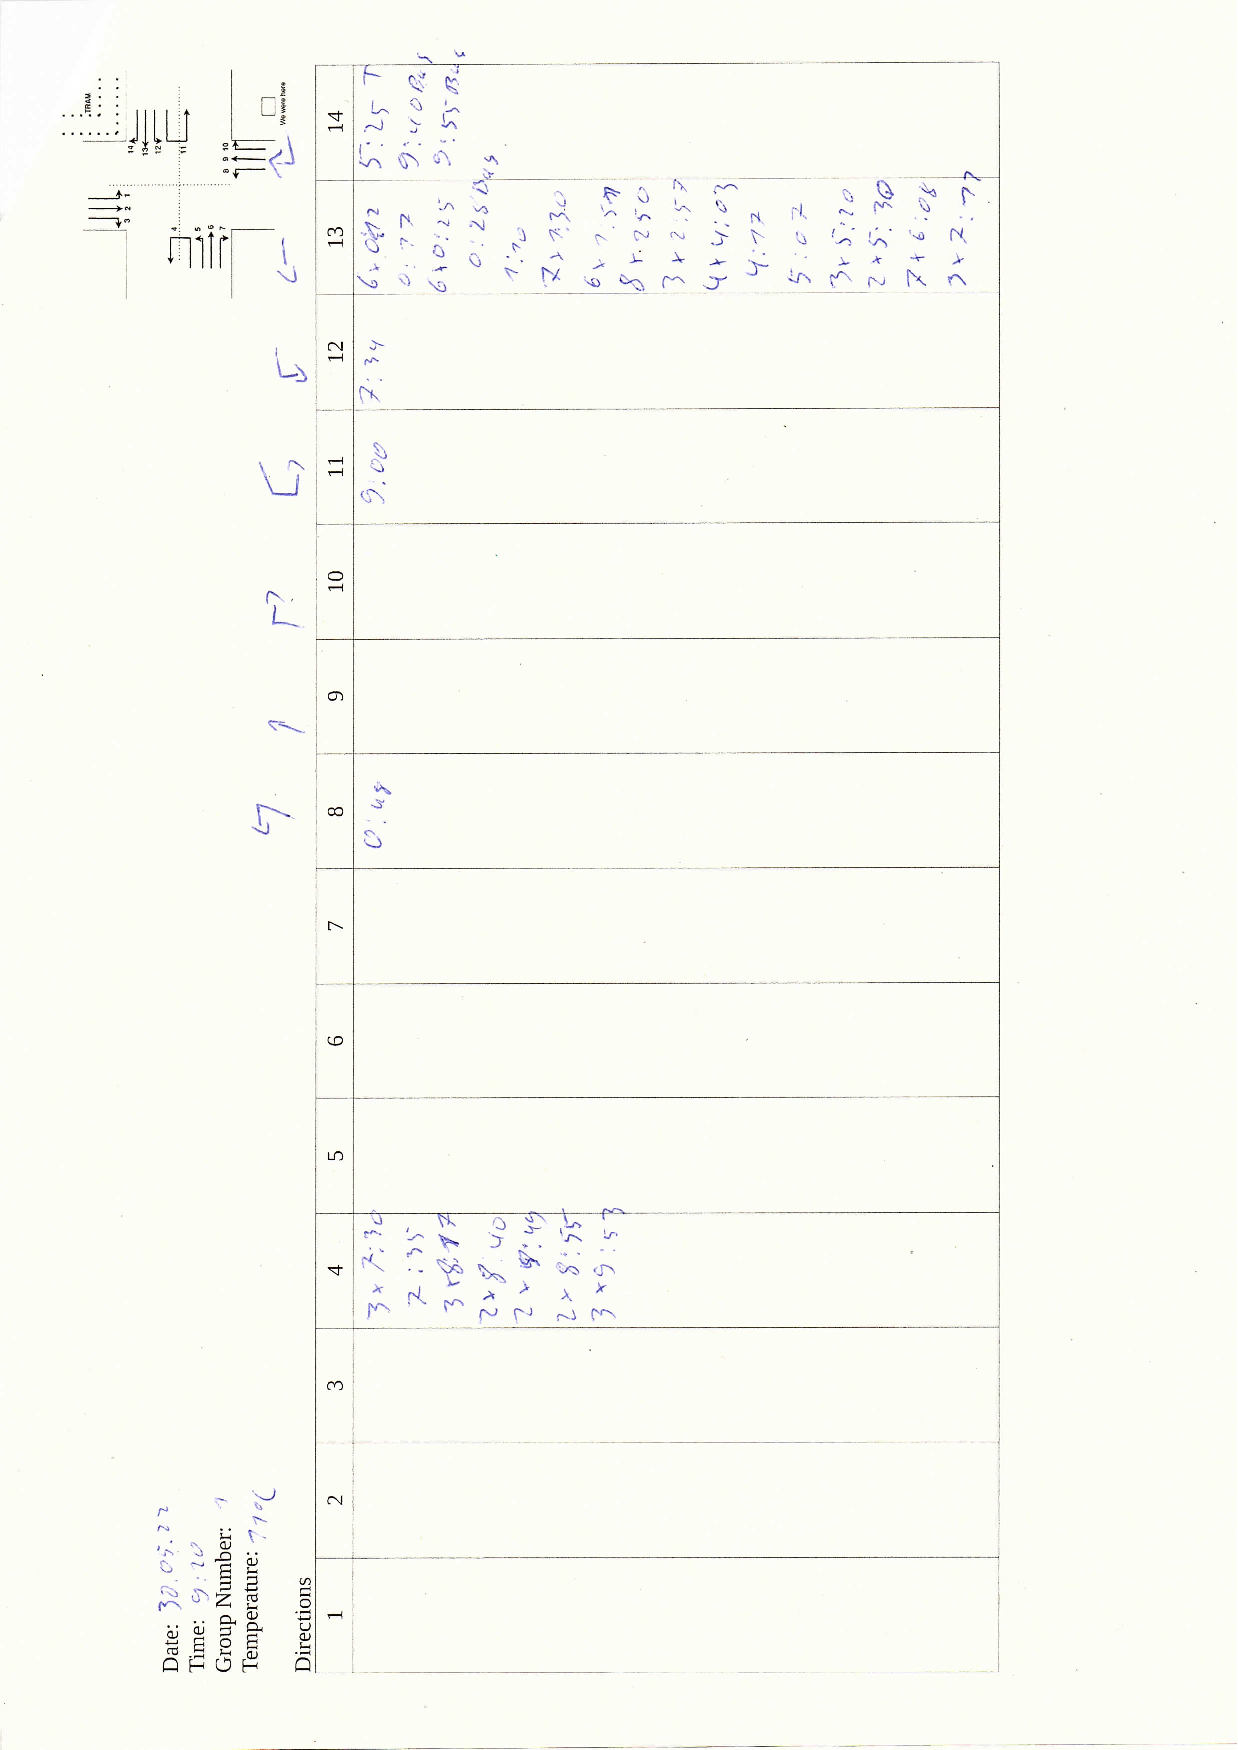
\includegraphics[]{scans/300522_0920.pdf}}}\\\\
%\rotatebox{270}{\scalebox{.25}{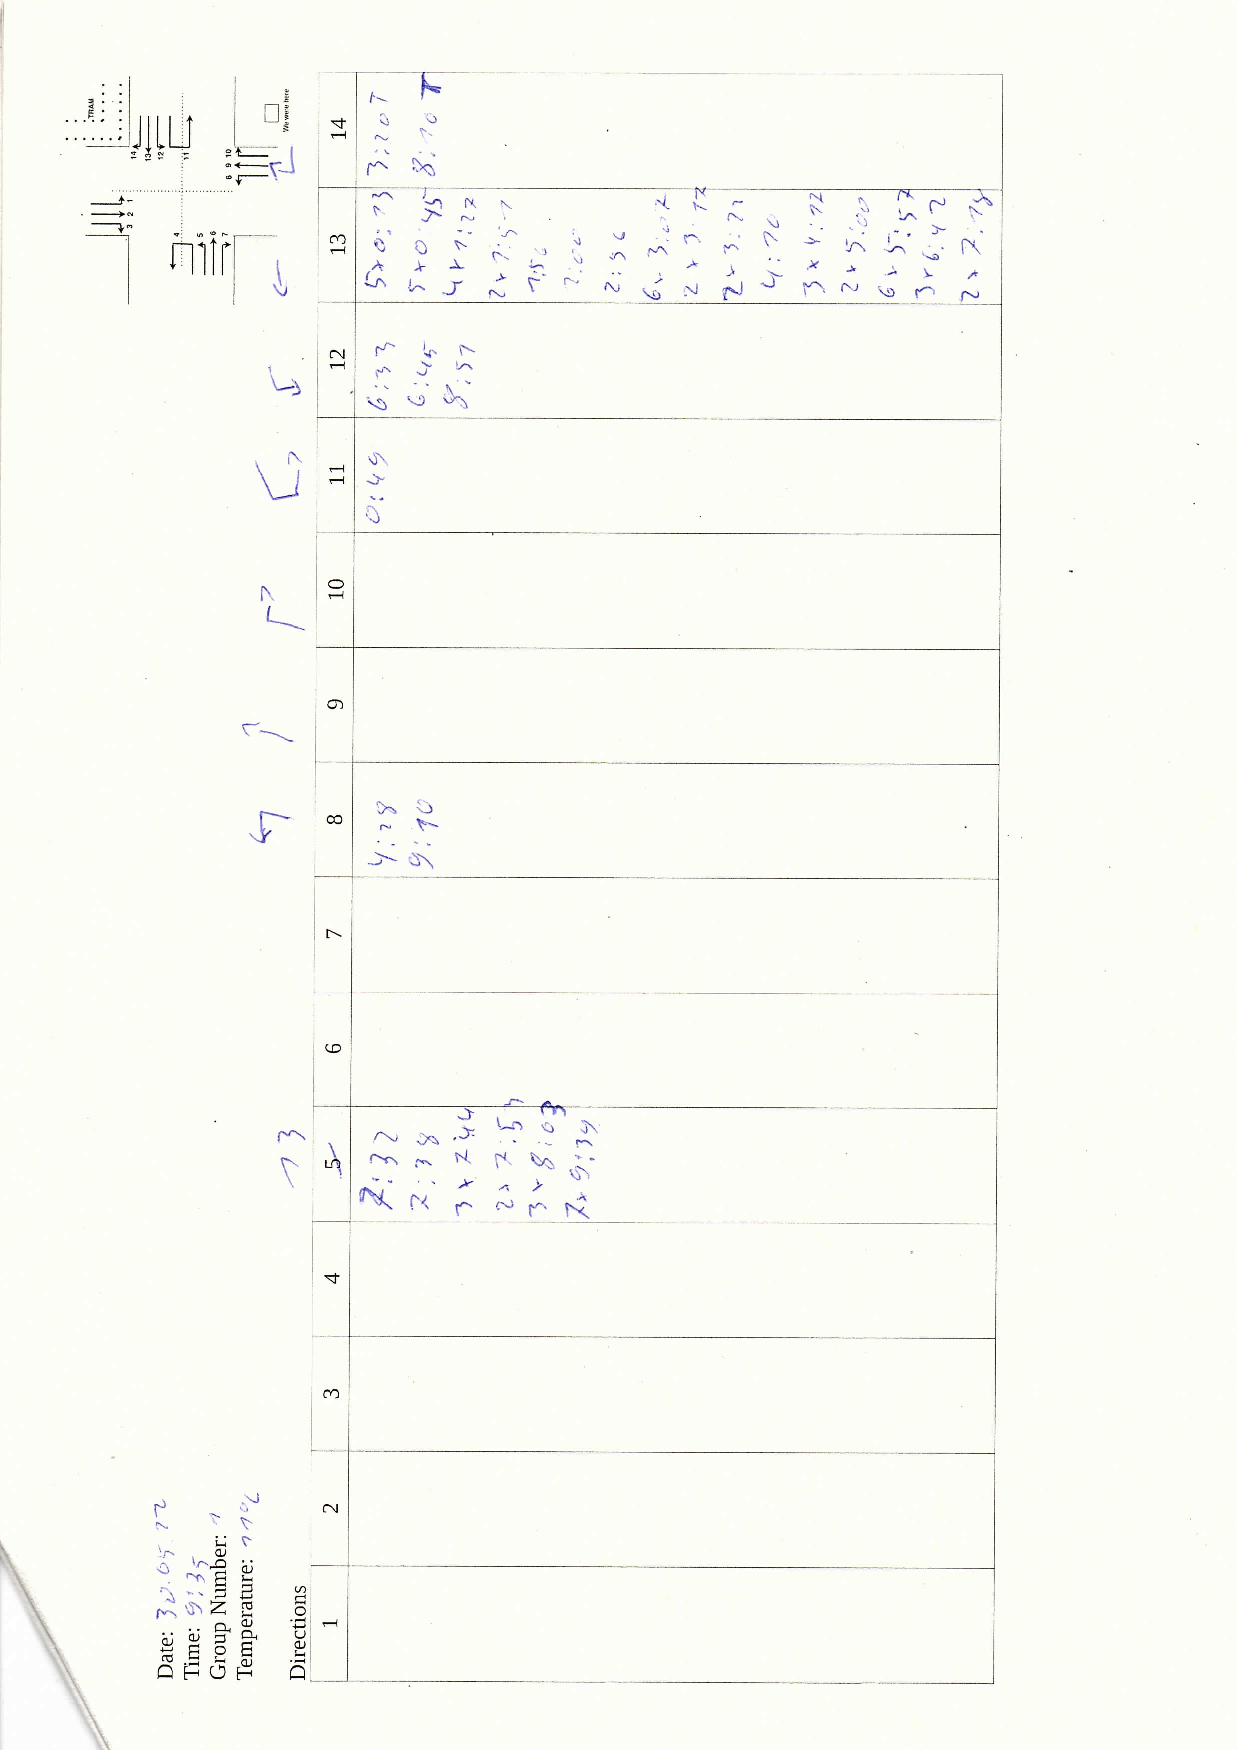
\includegraphics[]{scans/300522_0935.pdf}}}\\\\
%\rotatebox{270}{\scalebox{.25}{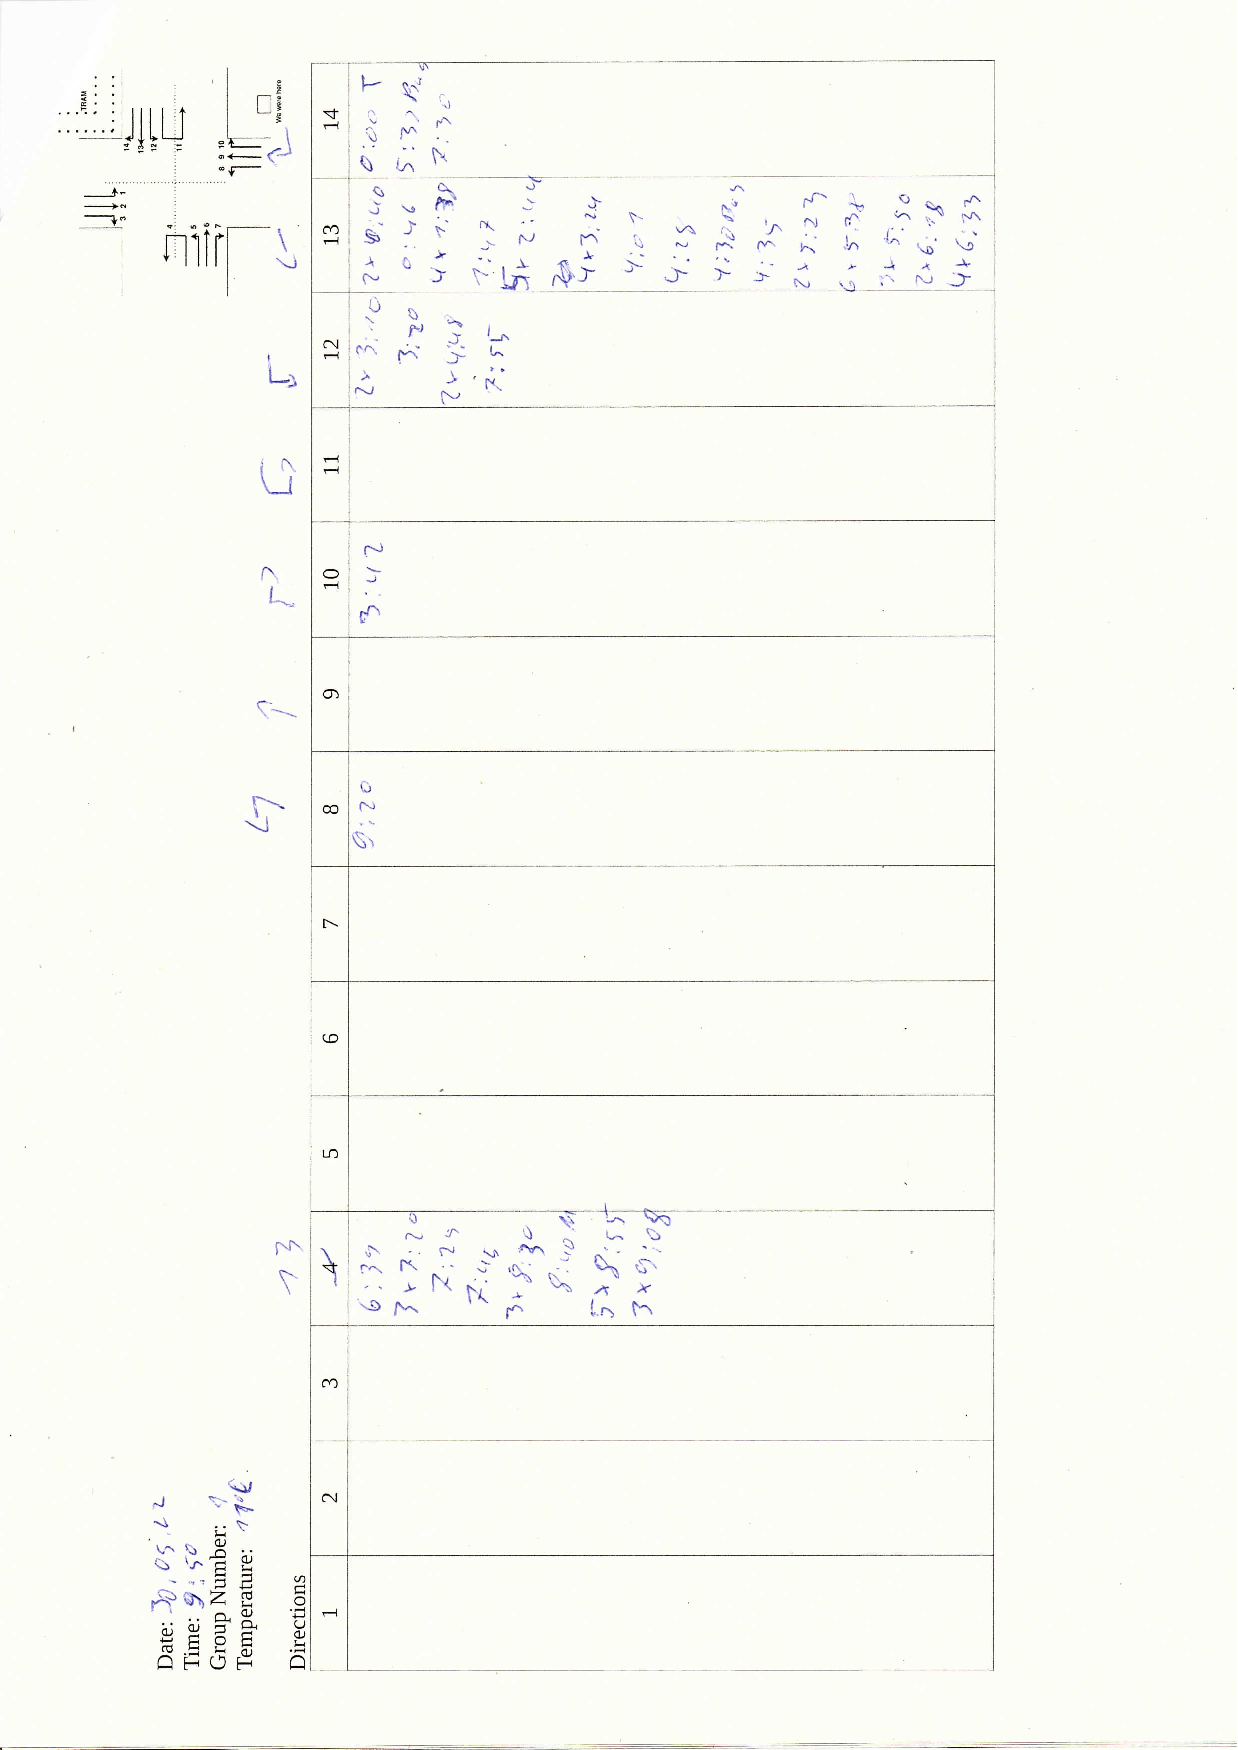
\includegraphics[]{scans/300522_0950.pdf}}}\\\\

\begin{figure*}[htbp]
  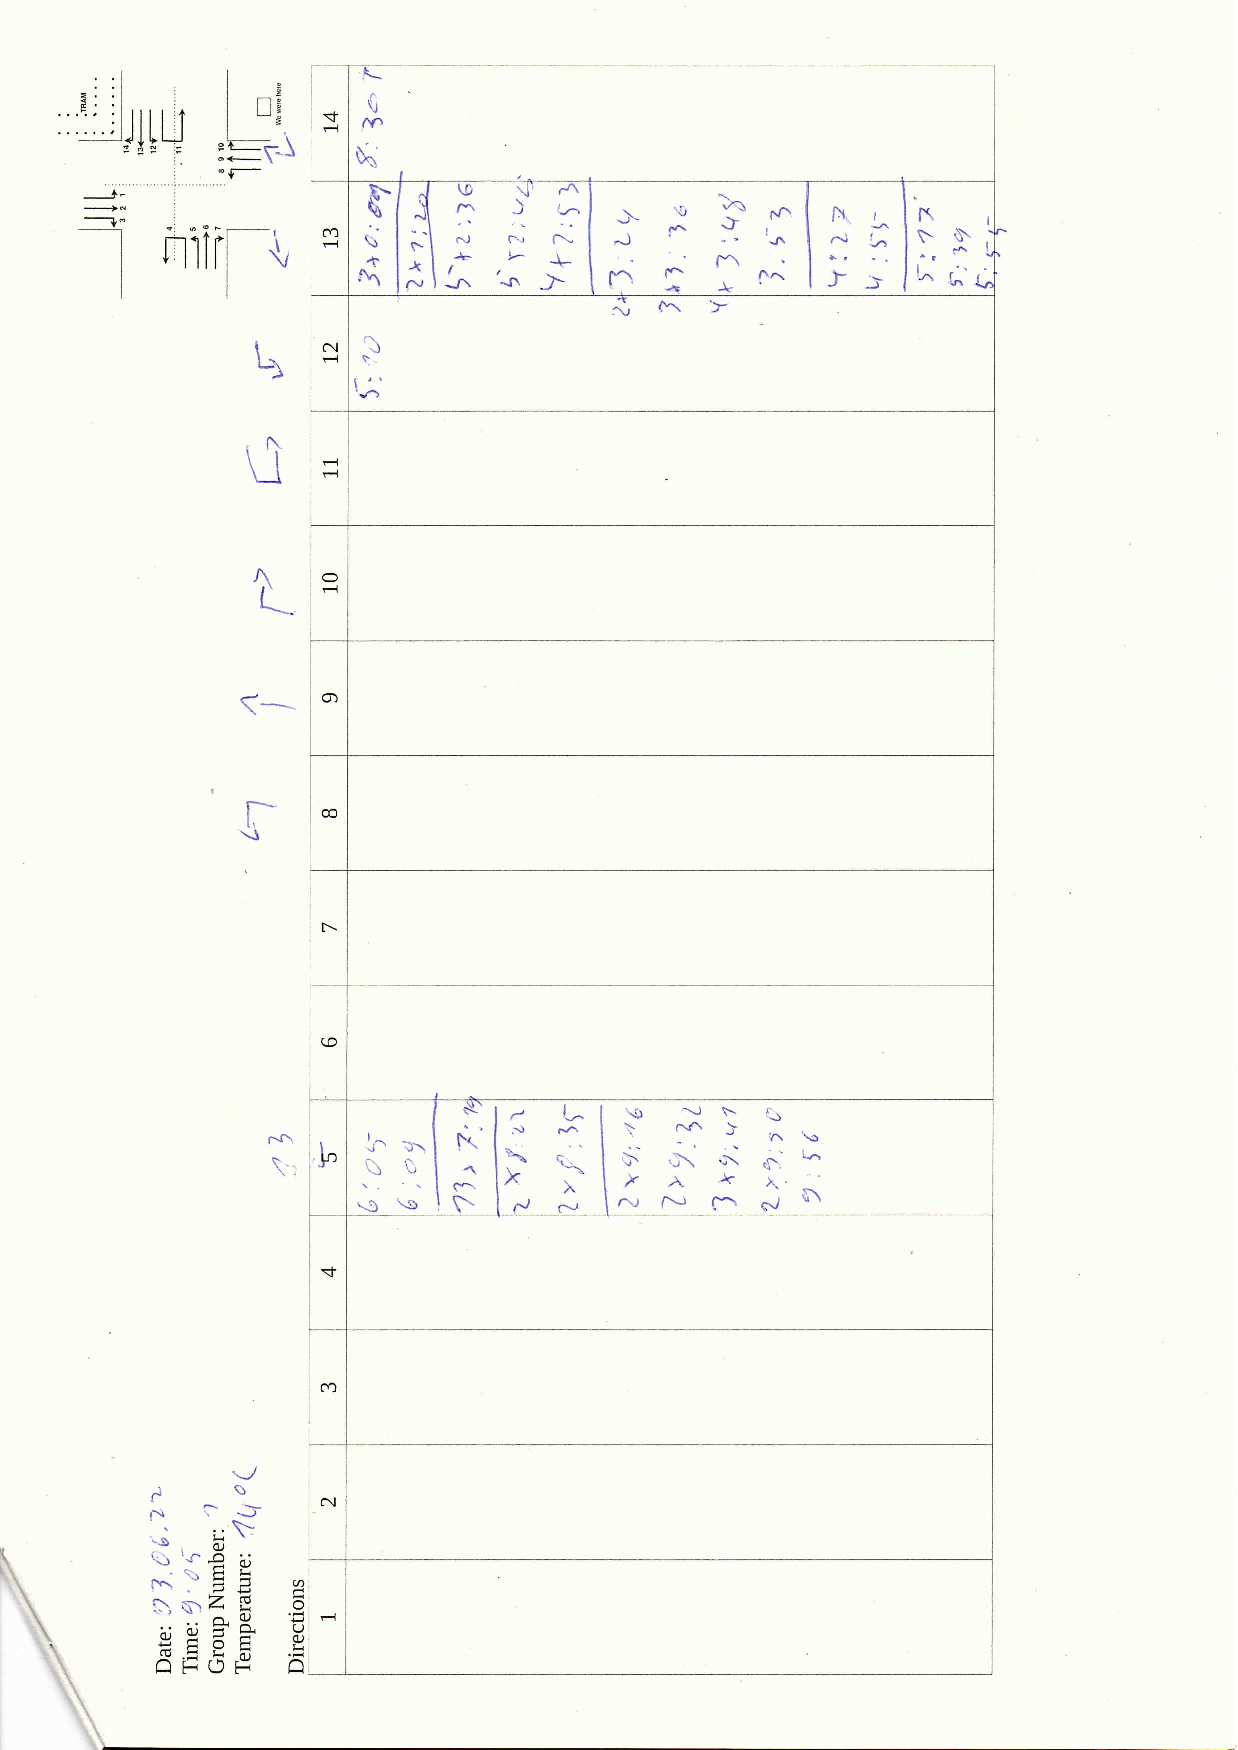
\includegraphics[width=\linewidth]{scans/030622_0905.pdf}
\end{figure*}

\begin{figure*}[htbp]
  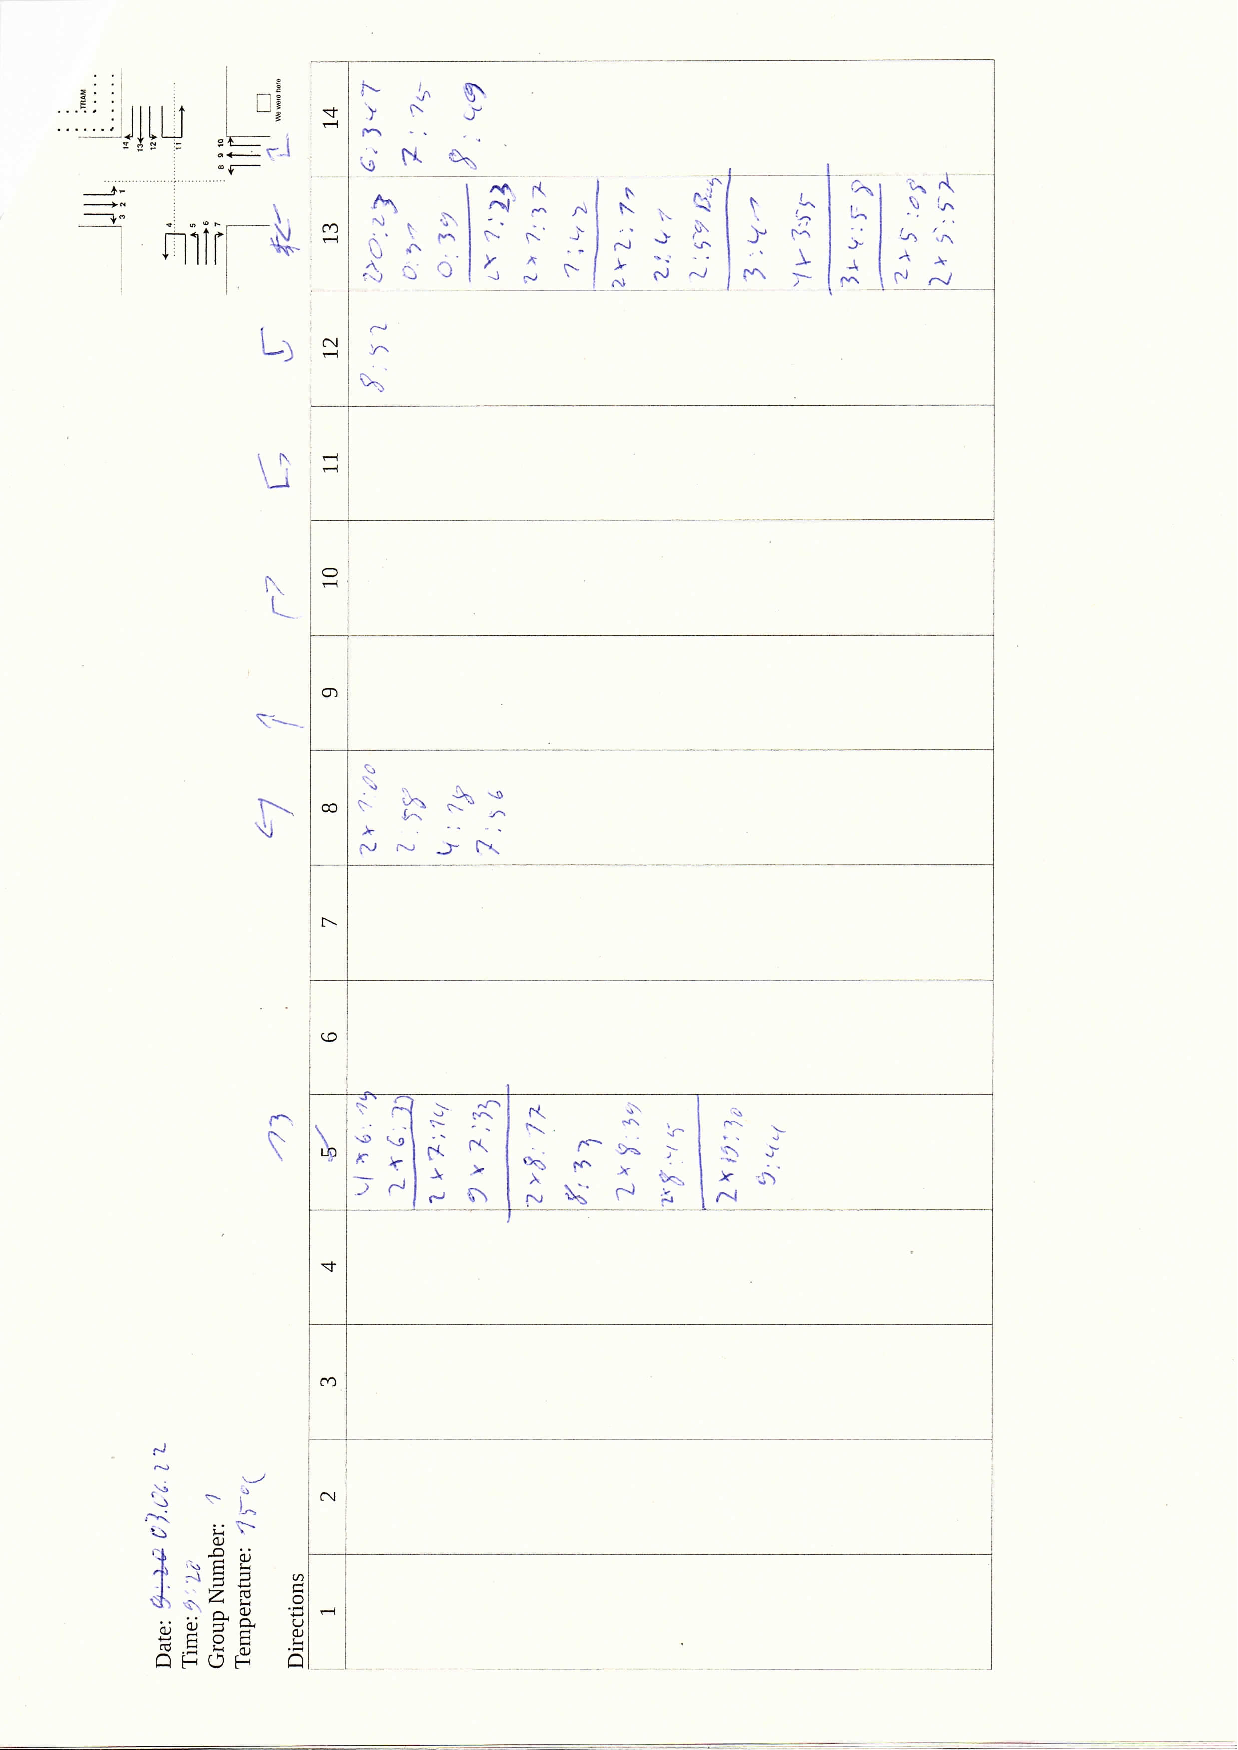
\includegraphics[width=\linewidth]{scans/030622_0920.pdf}
\end{figure*}

\begin{figure*}[htbp]
  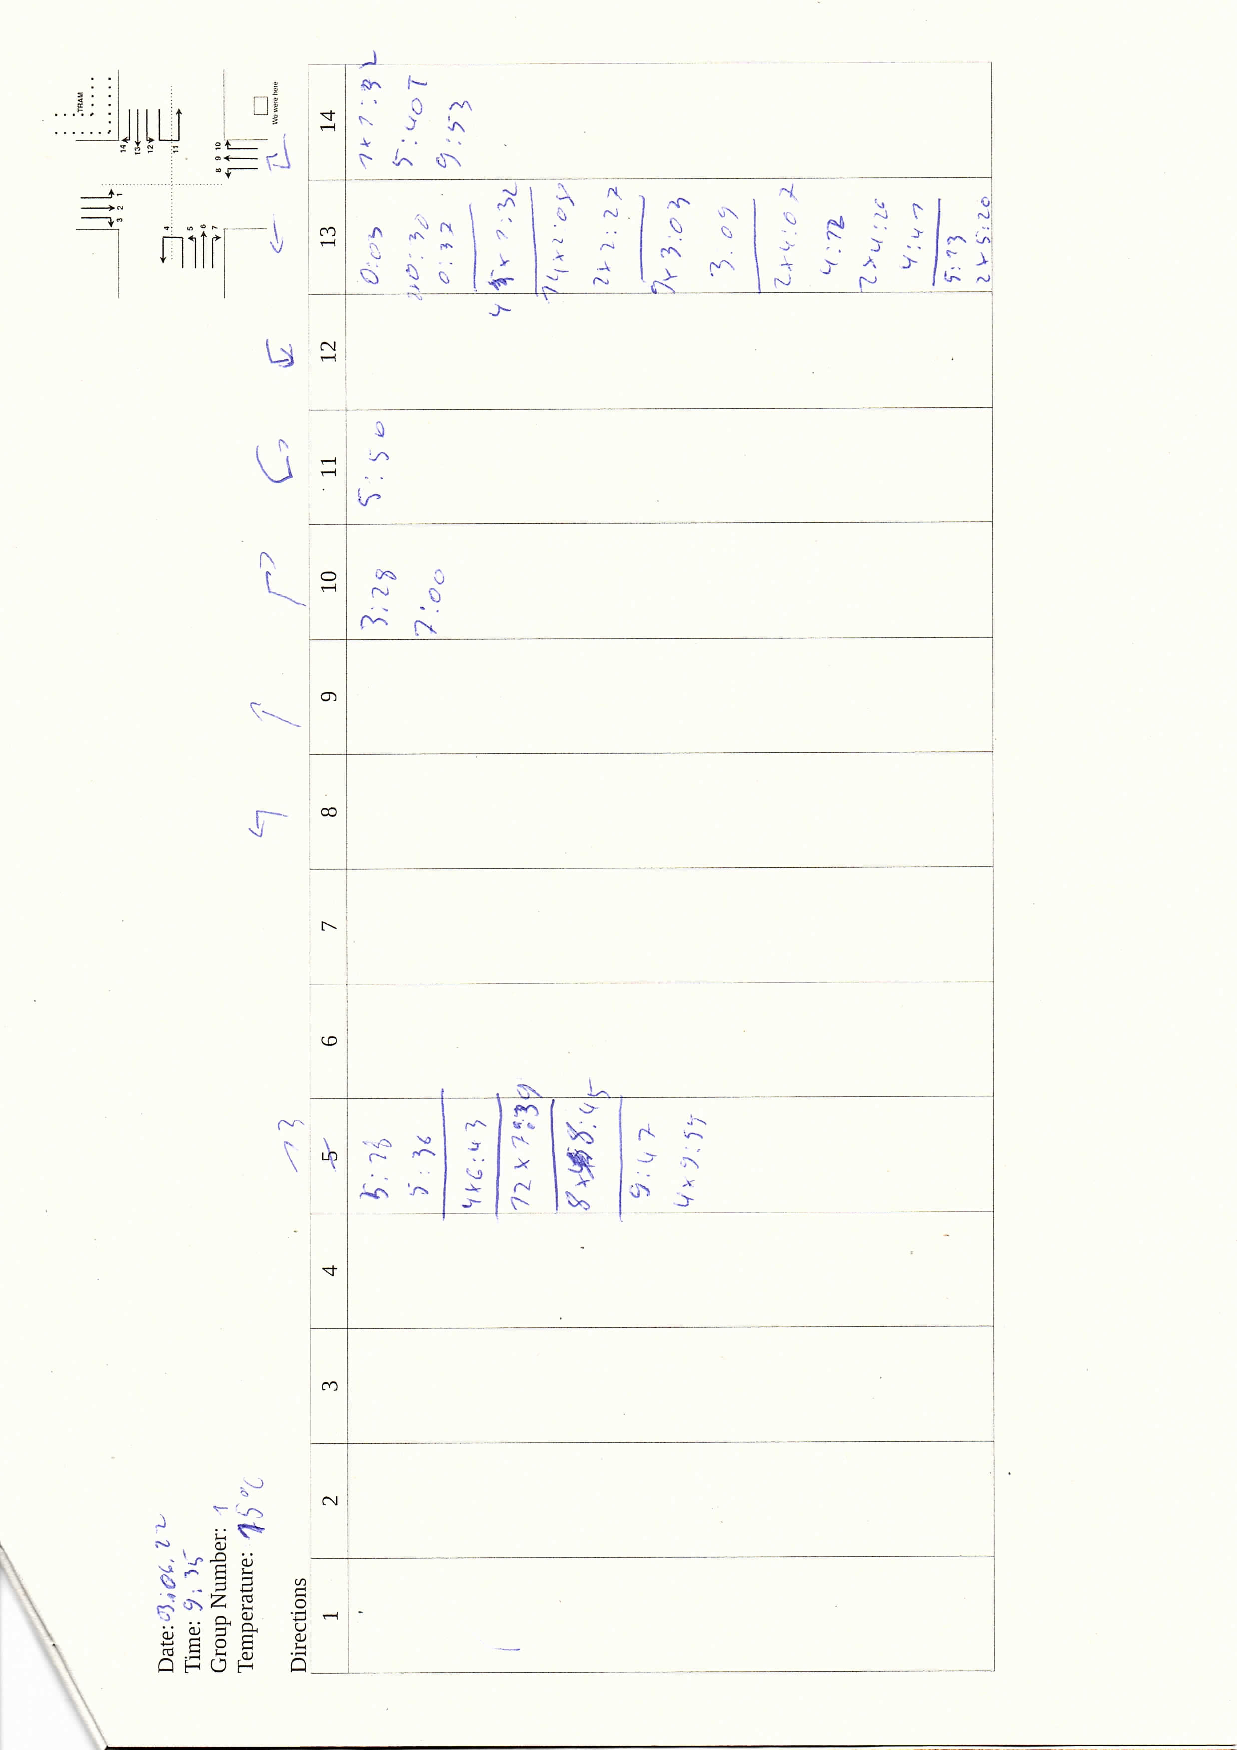
\includegraphics[width=\linewidth]{scans/030622_0935.pdf}
\end{figure*}

\begin{figure*}[htbp]
  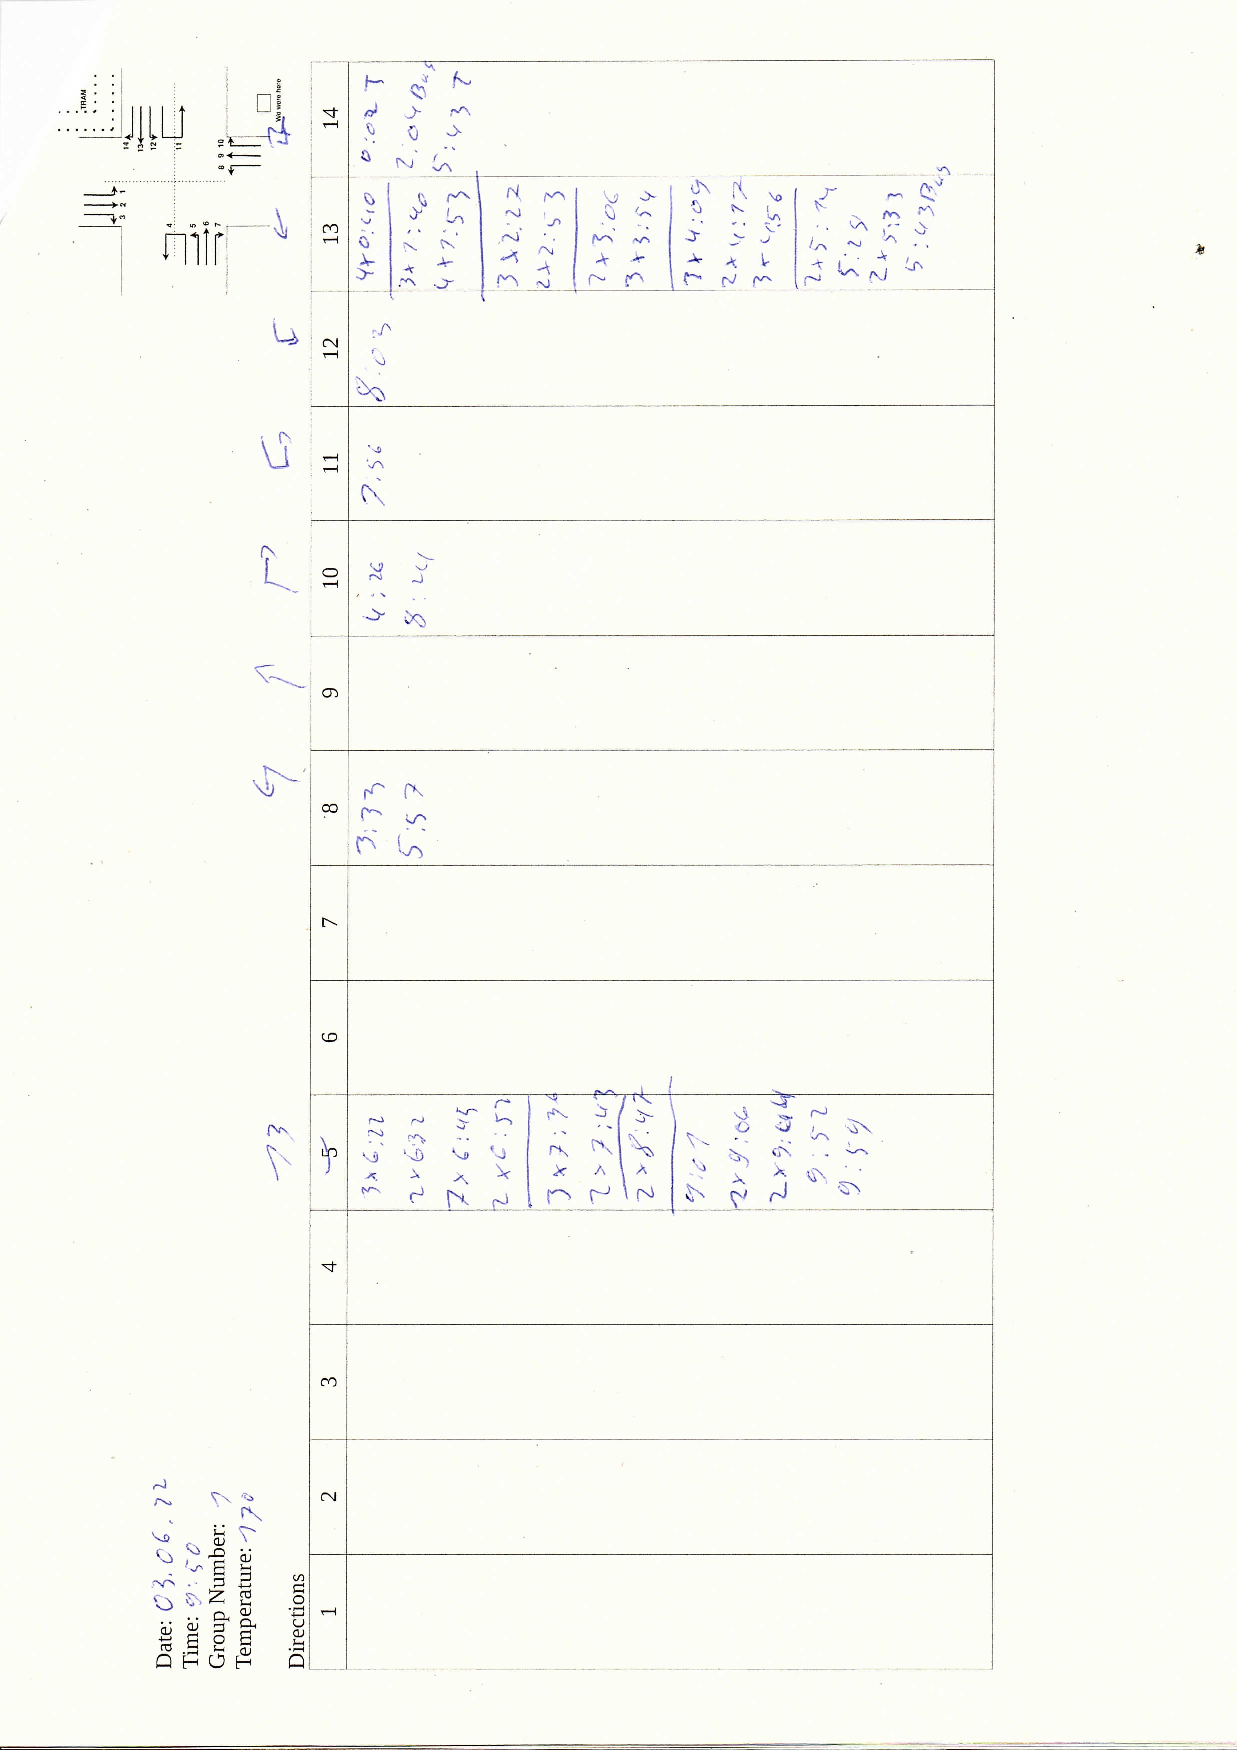
\includegraphics[width=\linewidth]{scans/030622_0950.pdf}
\end{figure*}

%\rotatebox{270}{\scalebox{.25}{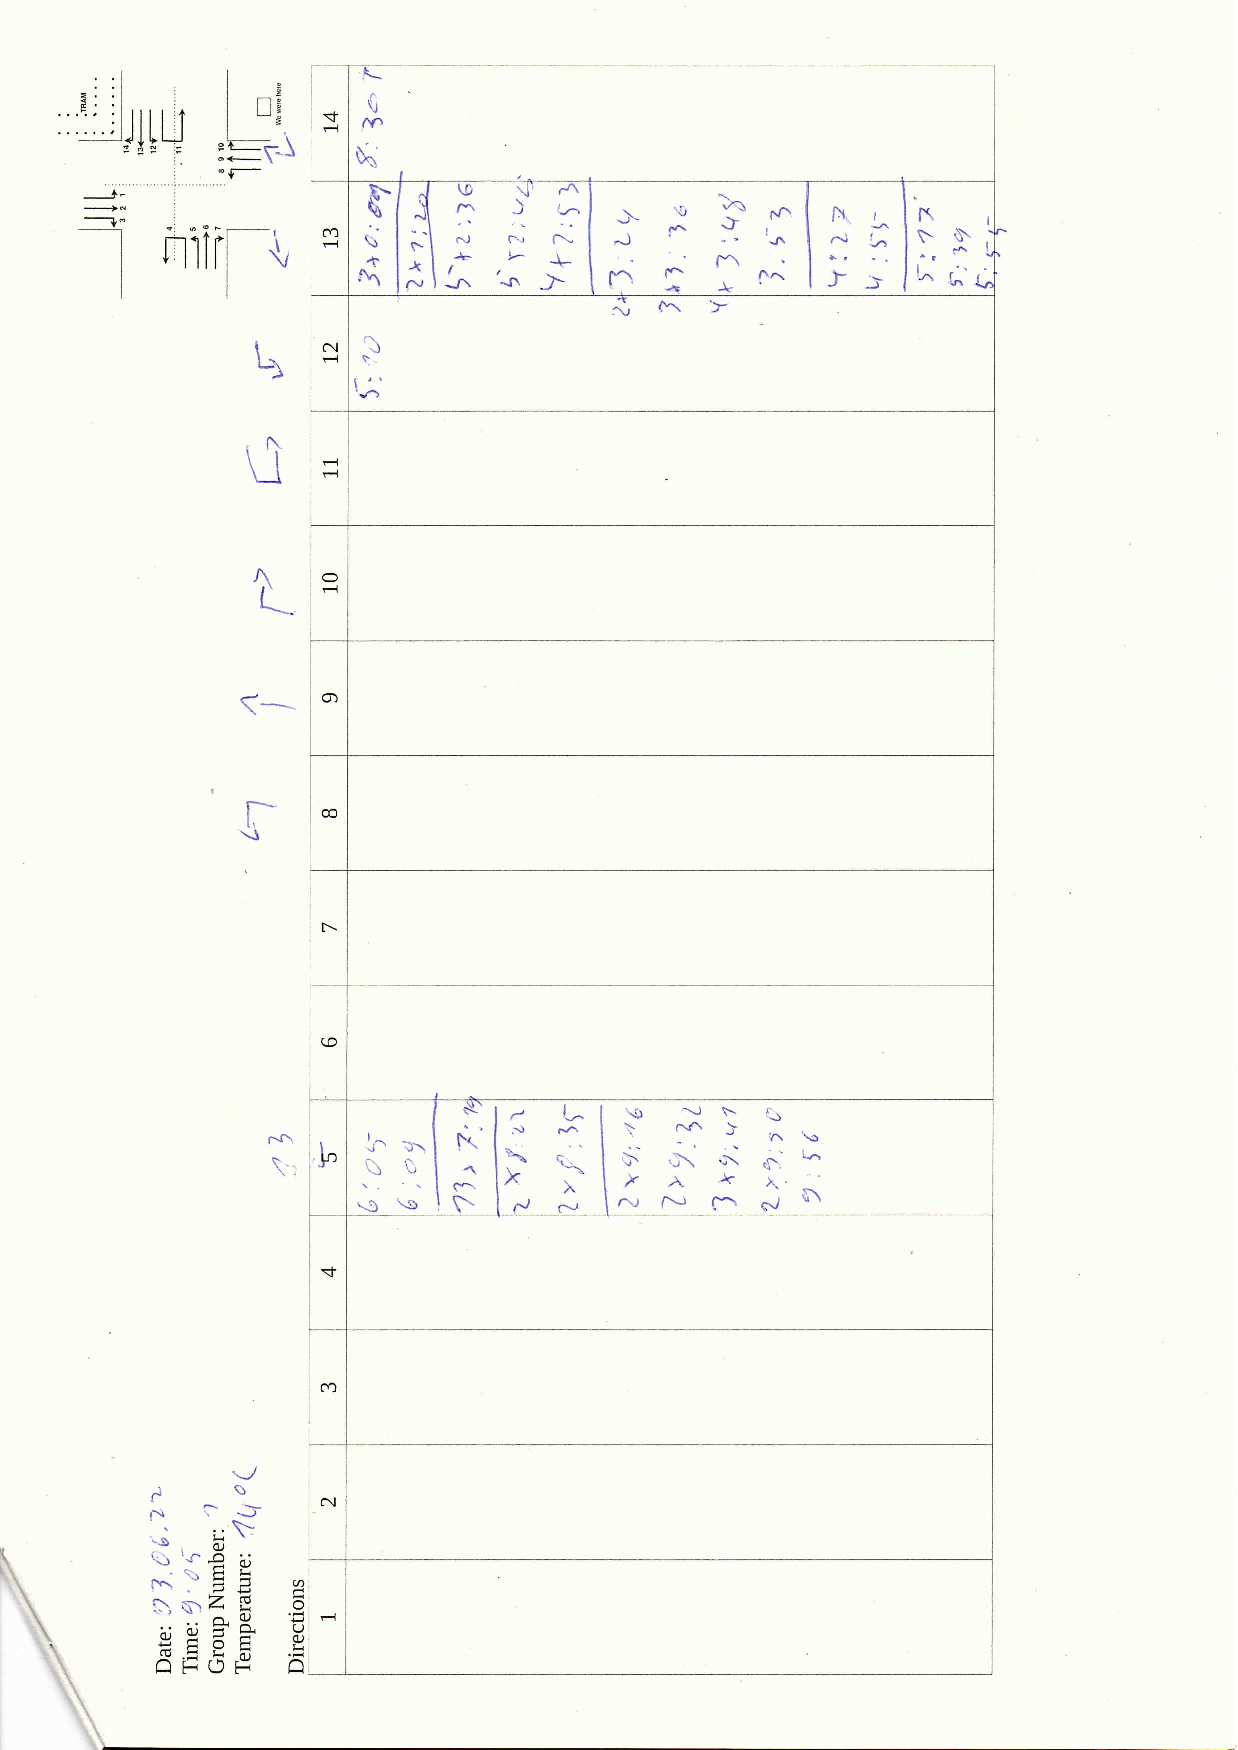
\includegraphics[]{scans/030622_0905.pdf}}}\\\\
%\rotatebox{270}{\scalebox{.25}{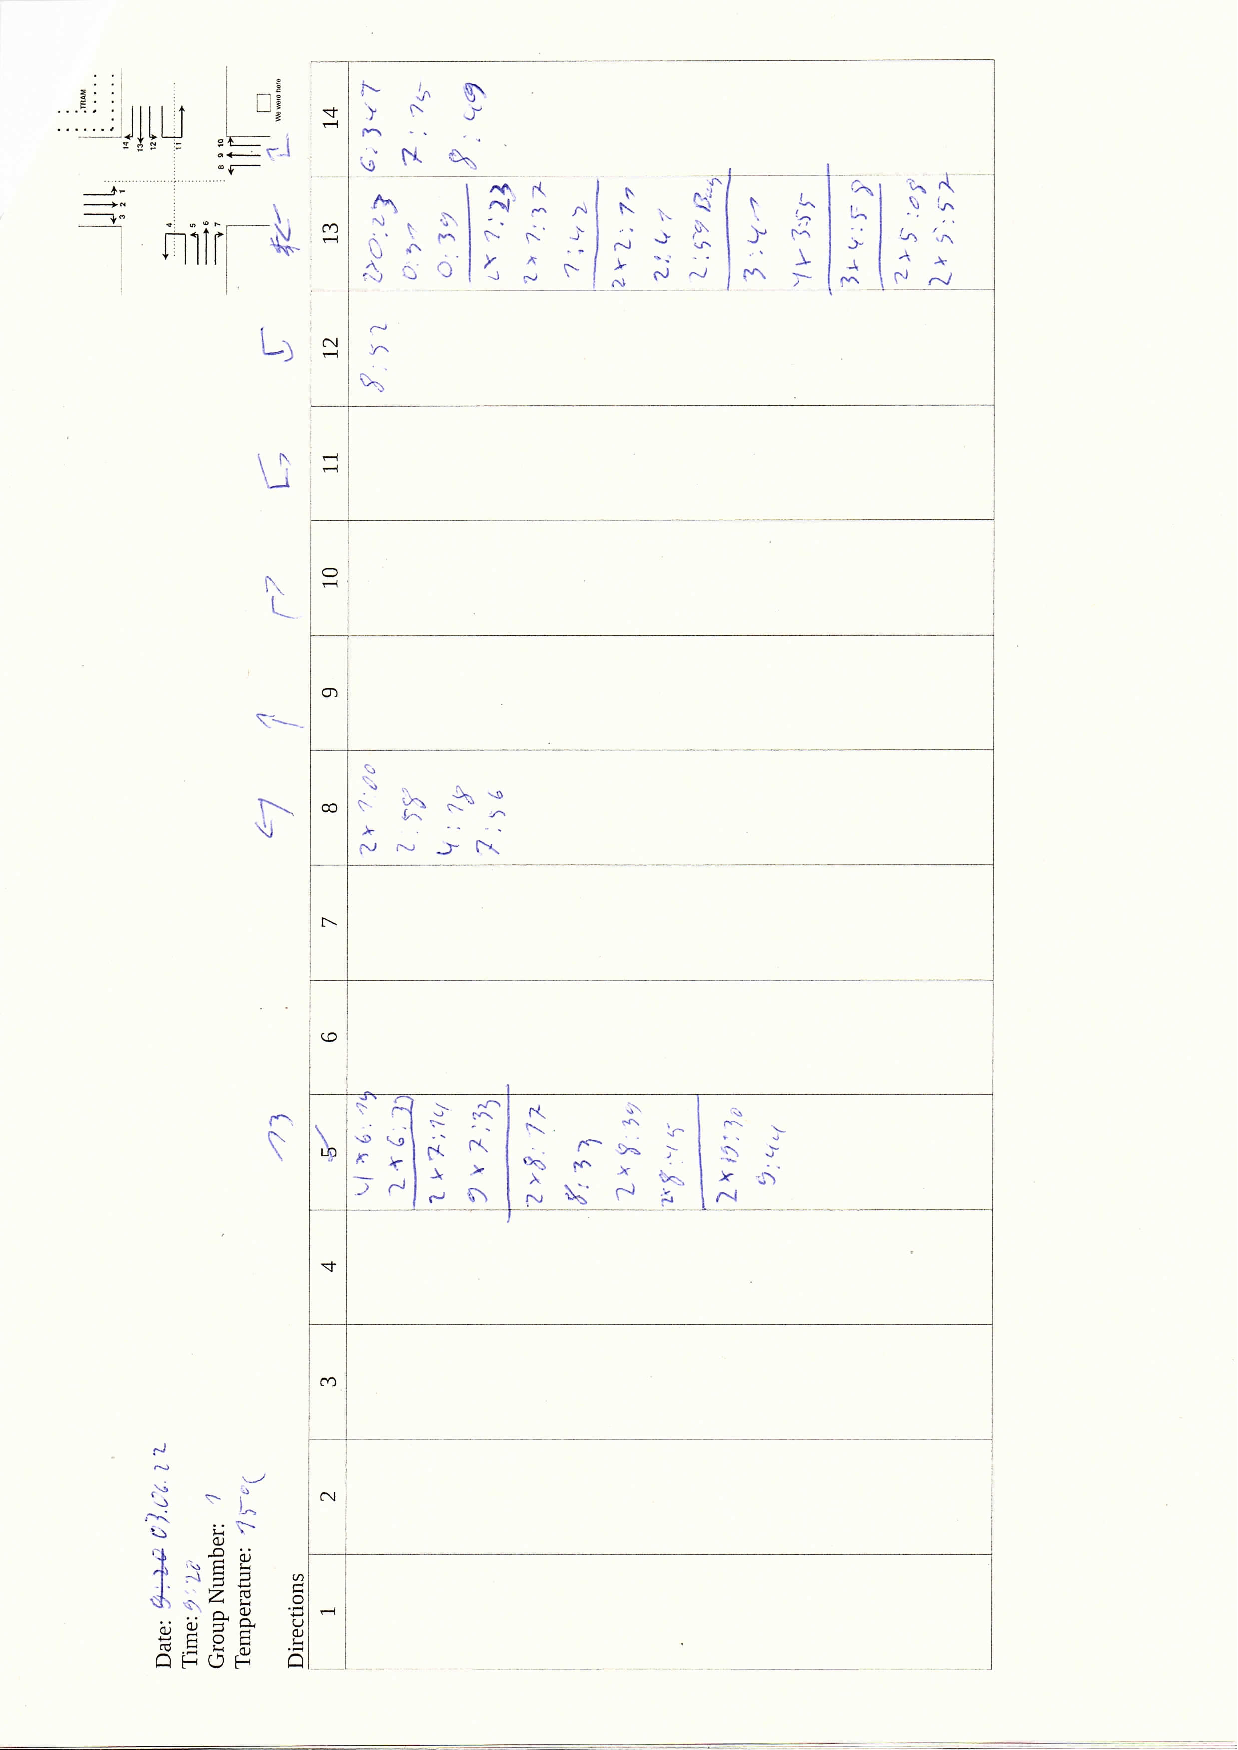
\includegraphics[]{scans/030622_0920.pdf}}}\\\\
%\rotatebox{270}{\scalebox{.25}{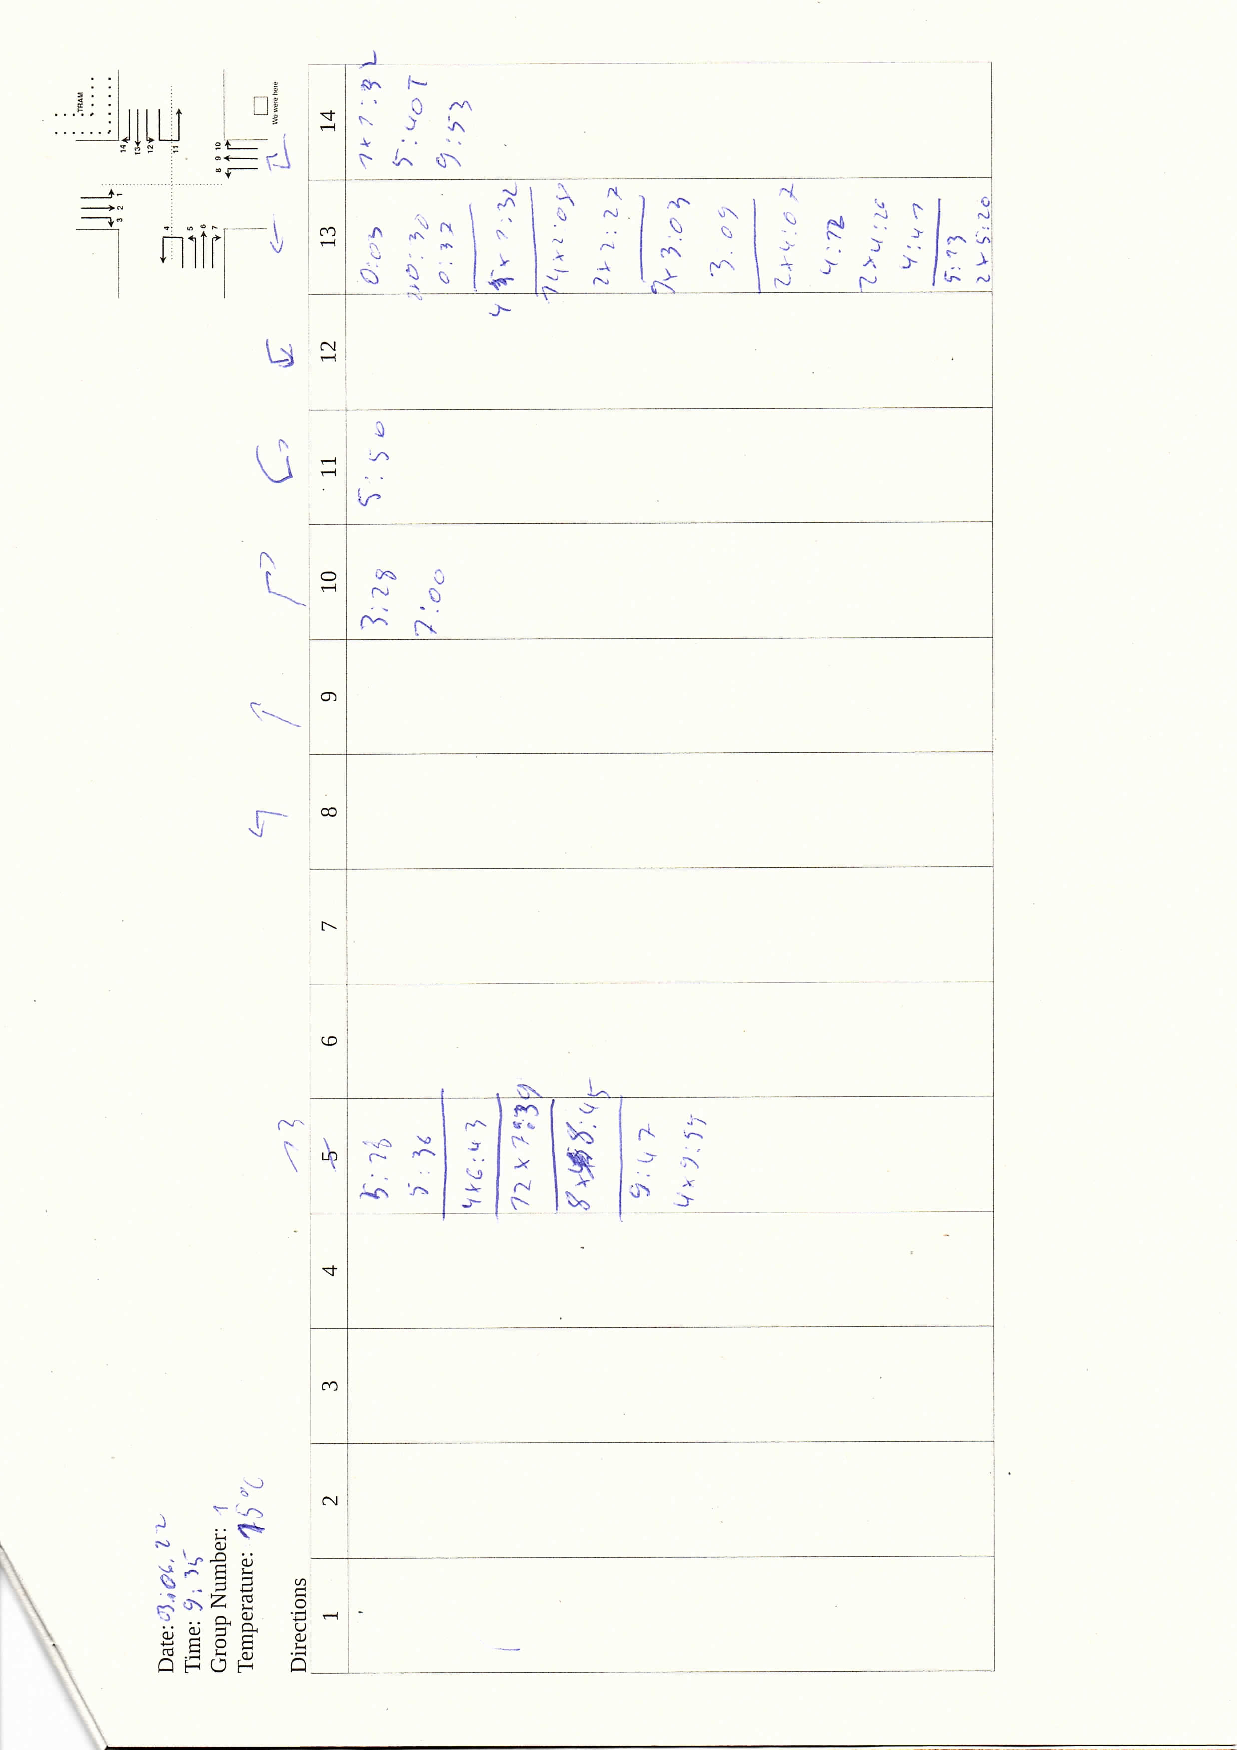
\includegraphics[]{scans/030622_0935.pdf}}}\\\\
%\rotatebox{270}{\scalebox{.25}{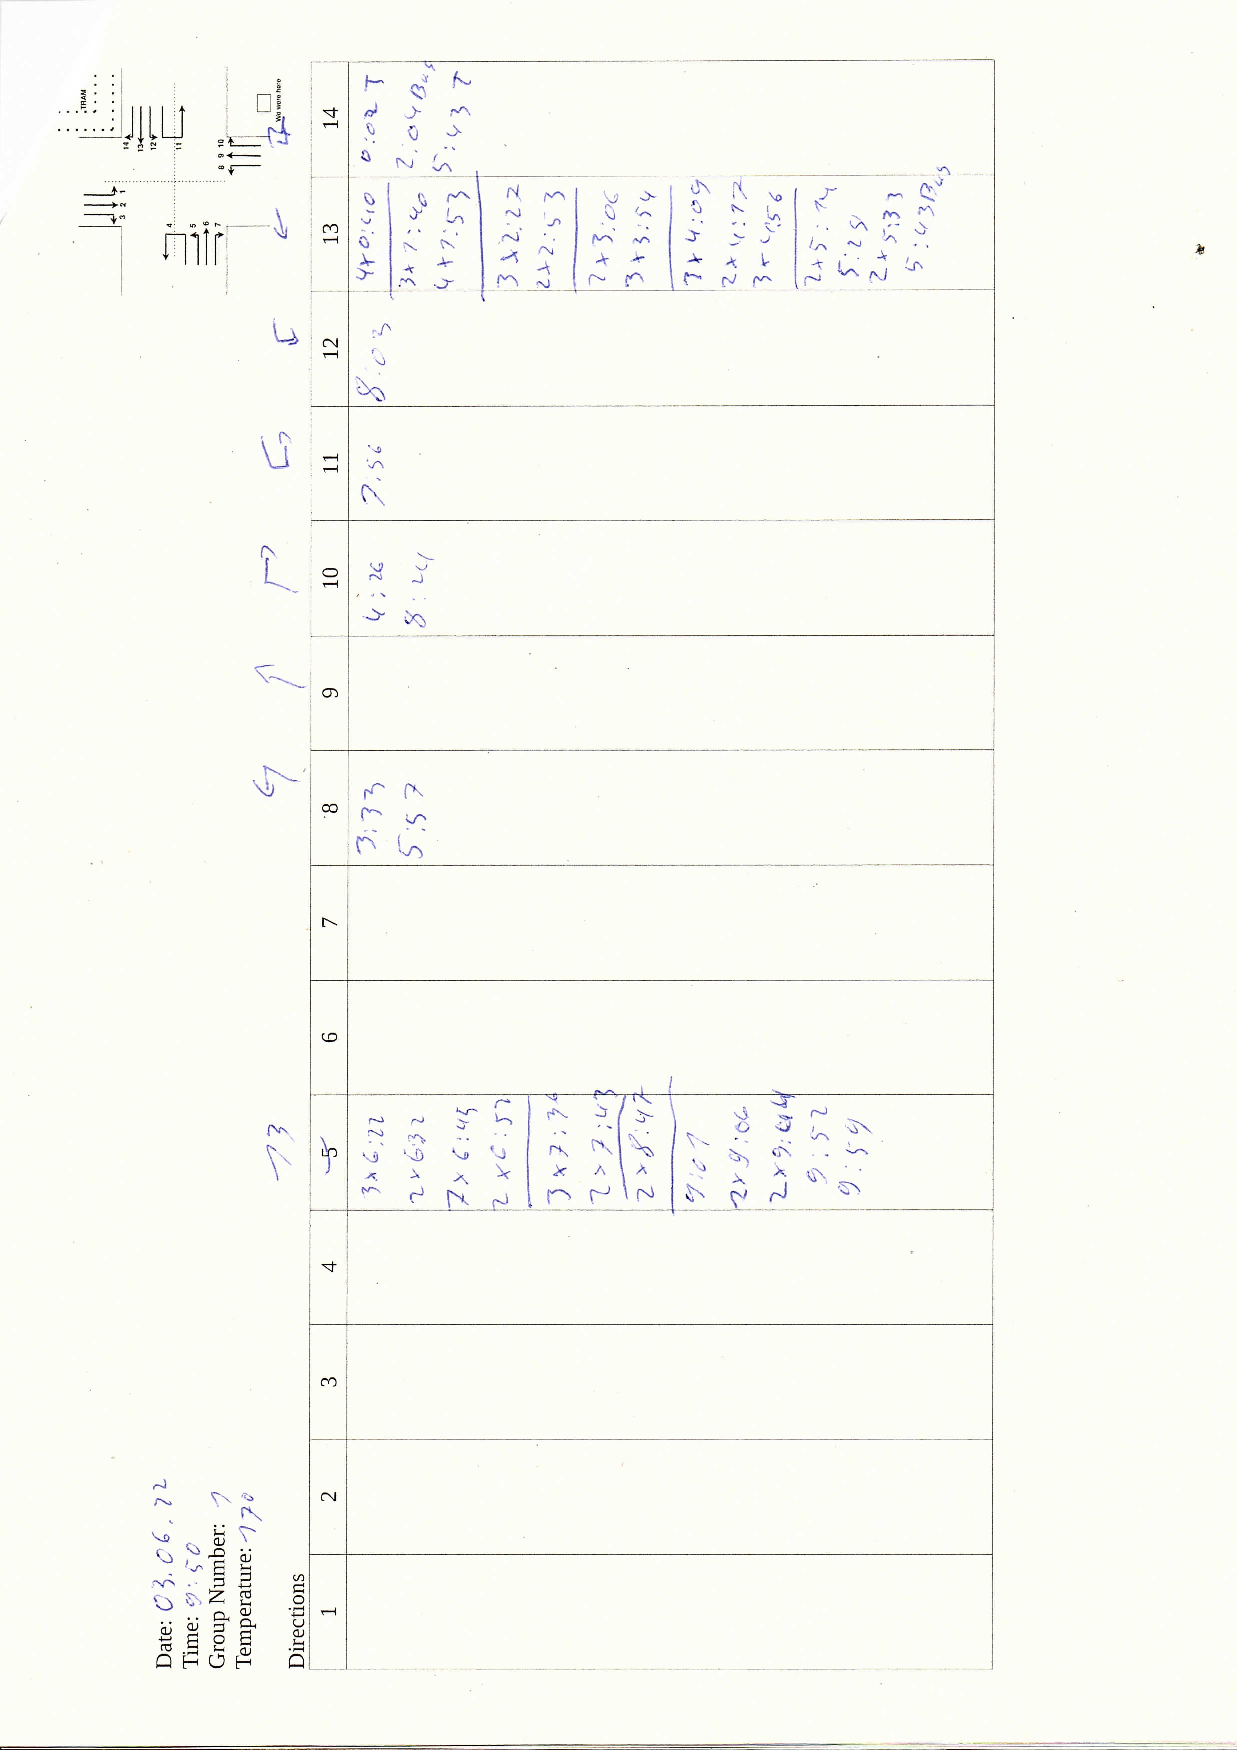
\includegraphics[]{scans/030622_0950.pdf}}}\\\\

\begin{figure*}[htbp]
  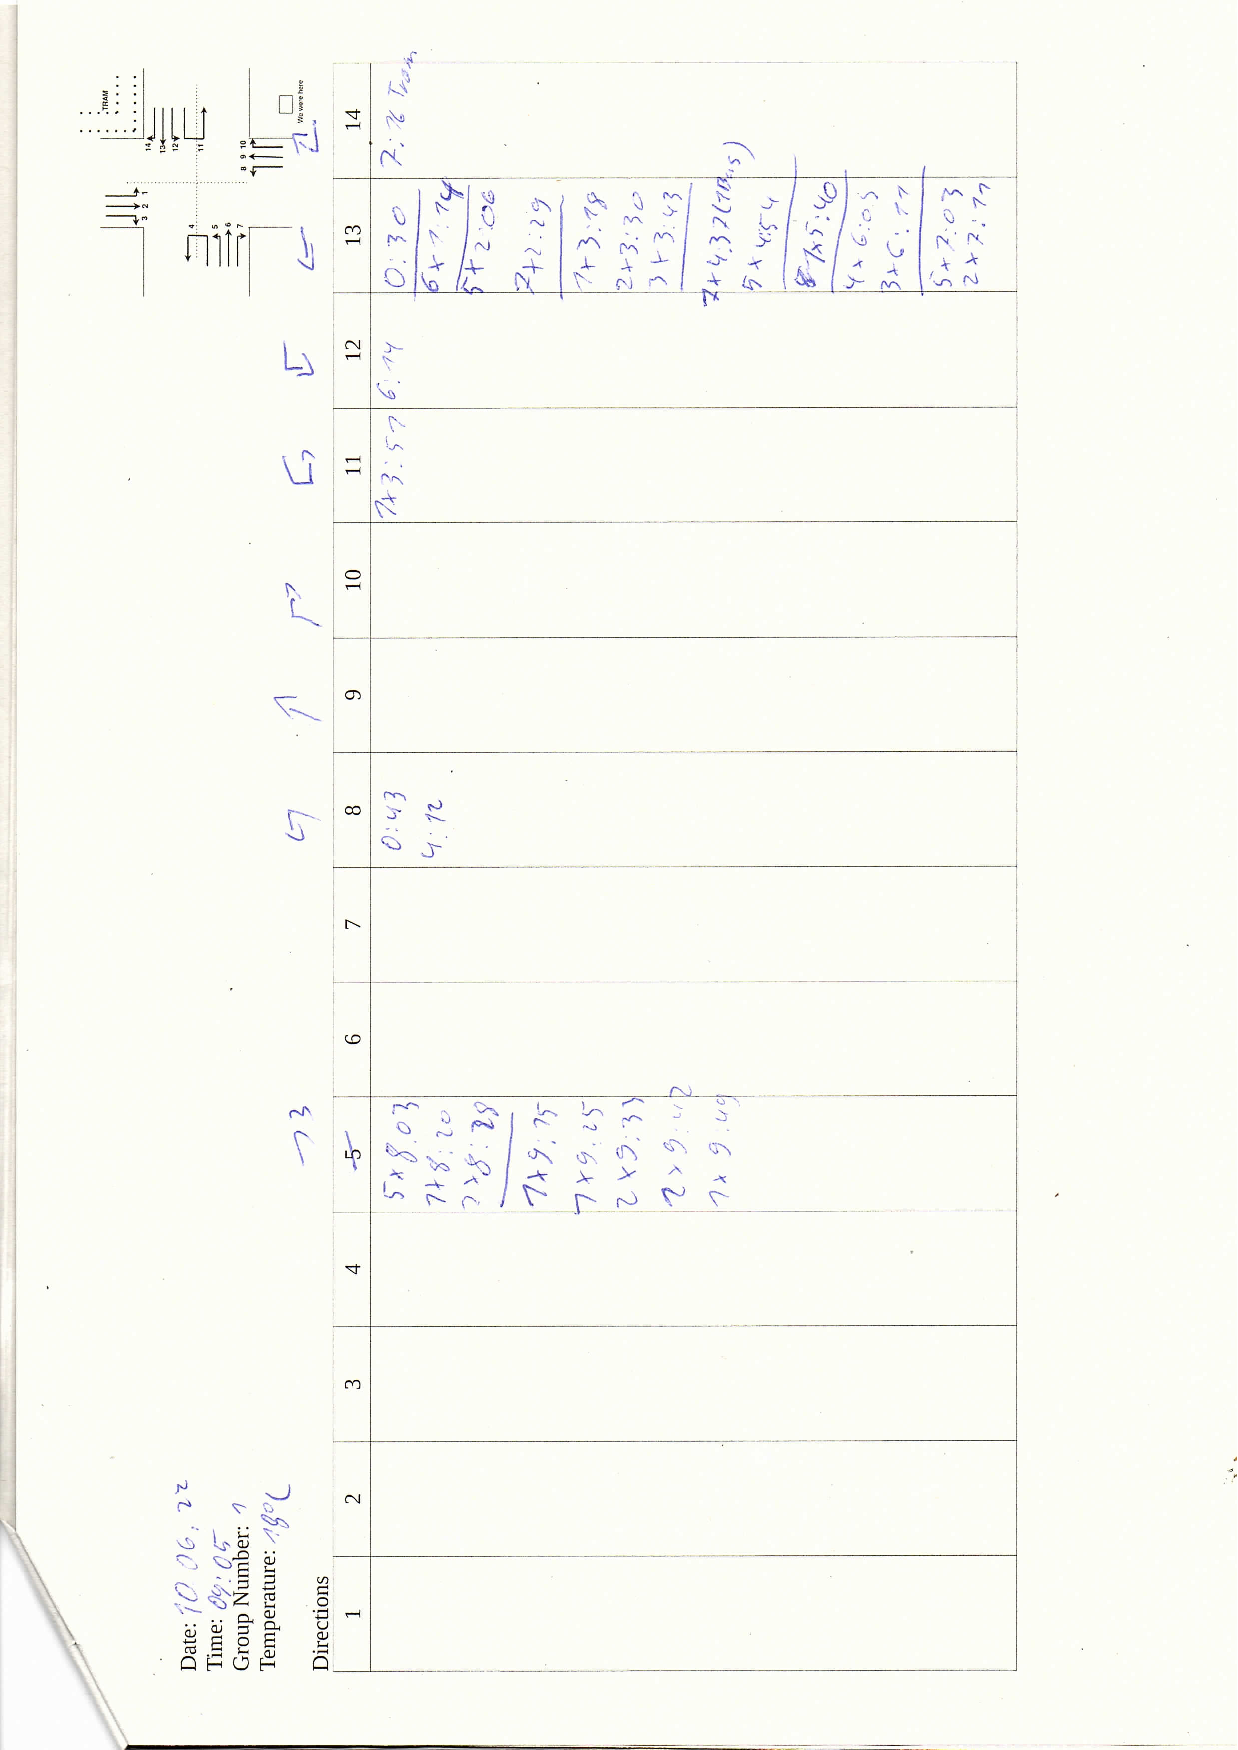
\includegraphics[width=\linewidth]{scans/100622_0905.pdf}
\end{figure*}

\begin{figure*}[htbp]
  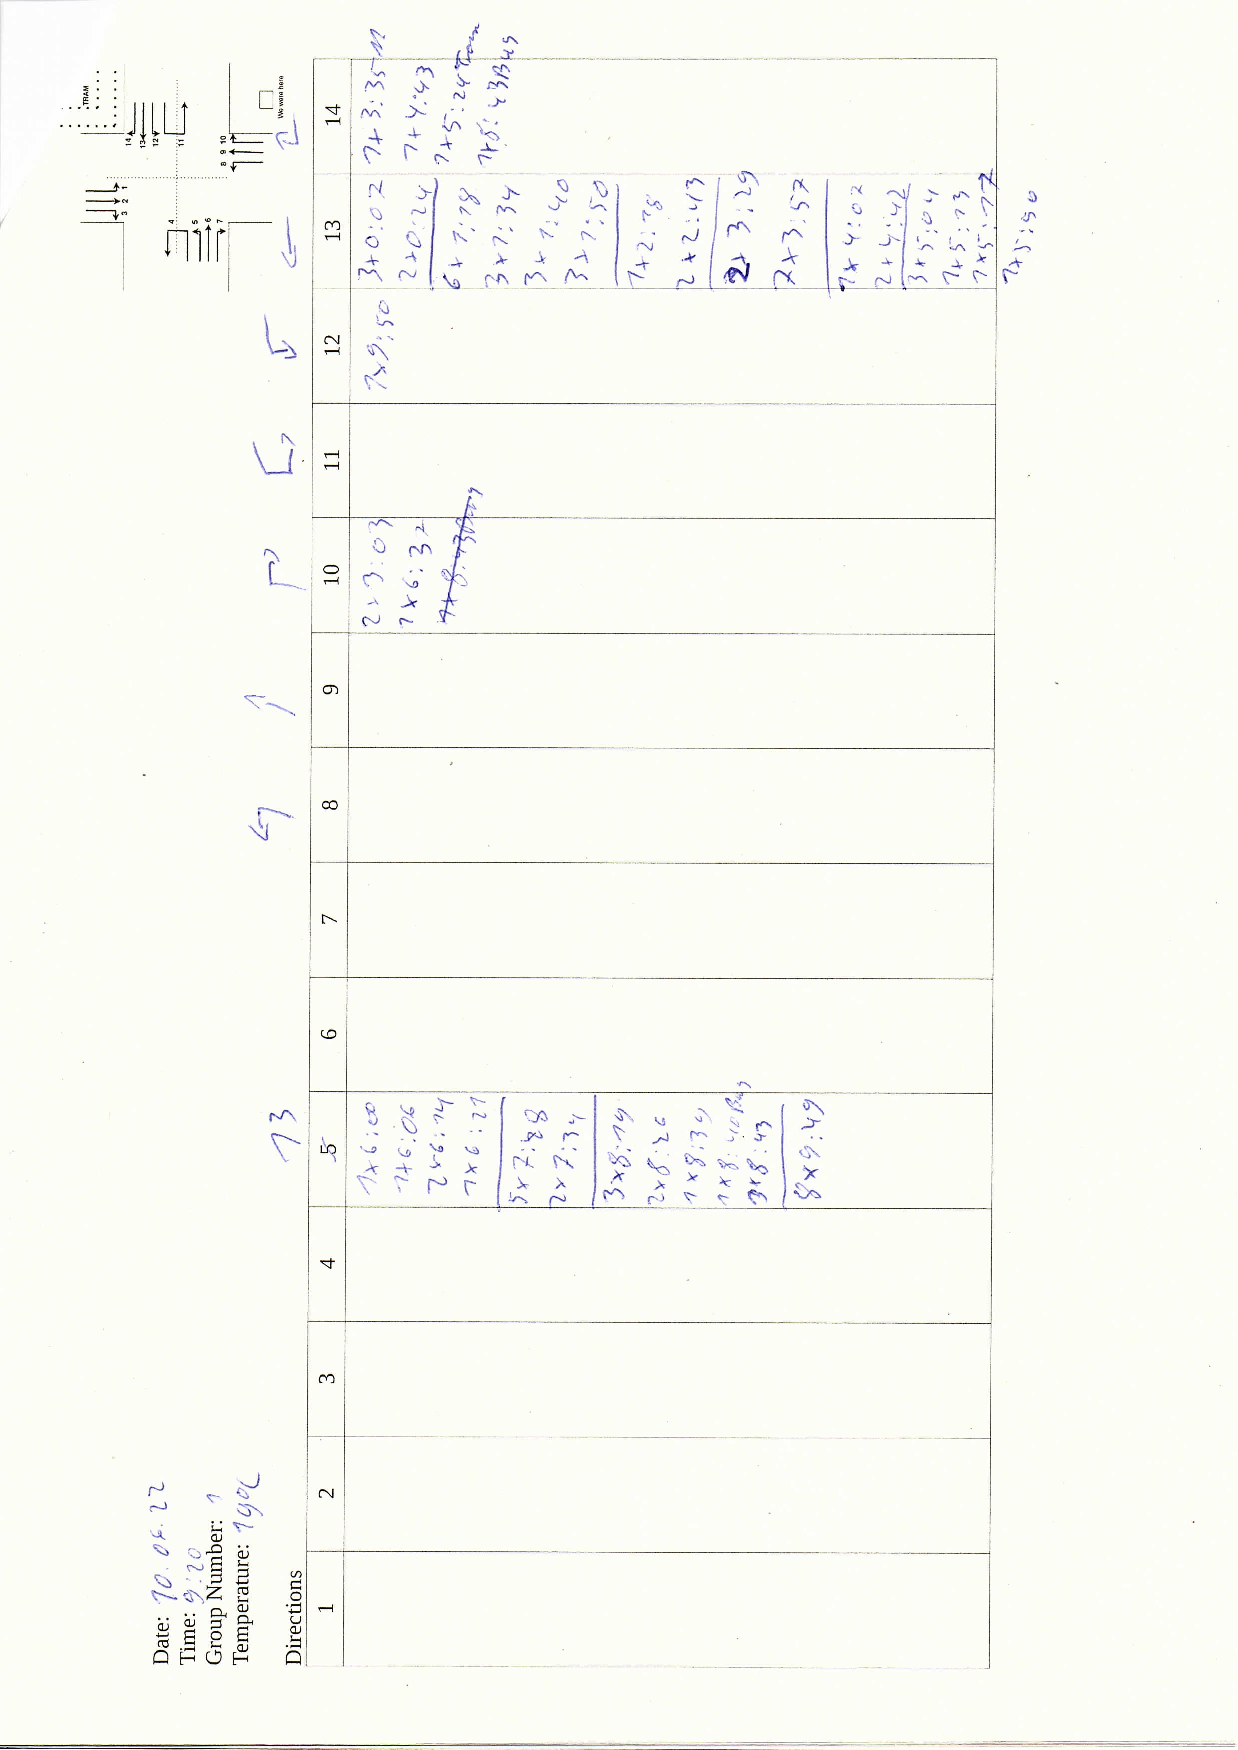
\includegraphics[width=\linewidth]{scans/100622_0920.pdf}
\end{figure*}

\begin{figure*}[htbp]
  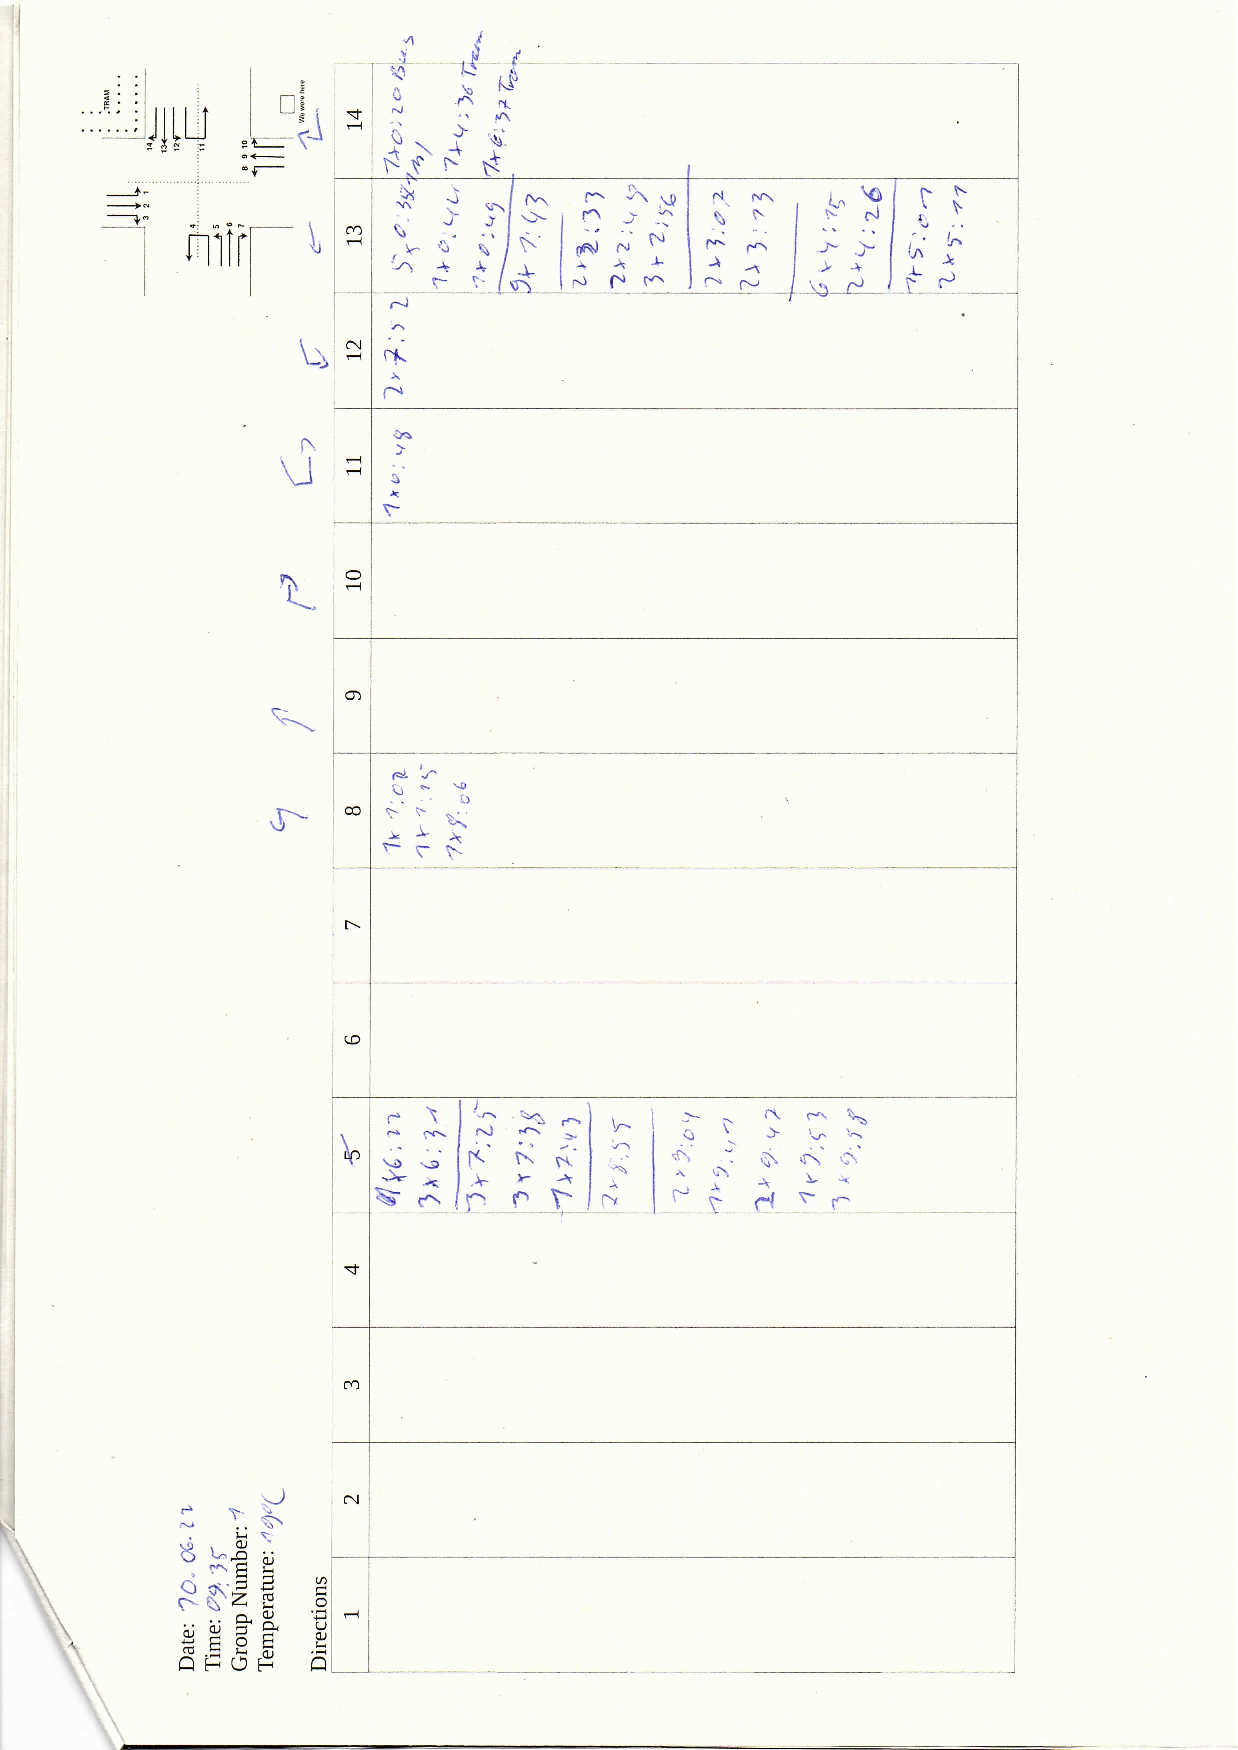
\includegraphics[width=\linewidth]{scans/100622_0935.pdf}
\end{figure*}

\begin{figure*}[htbp]
  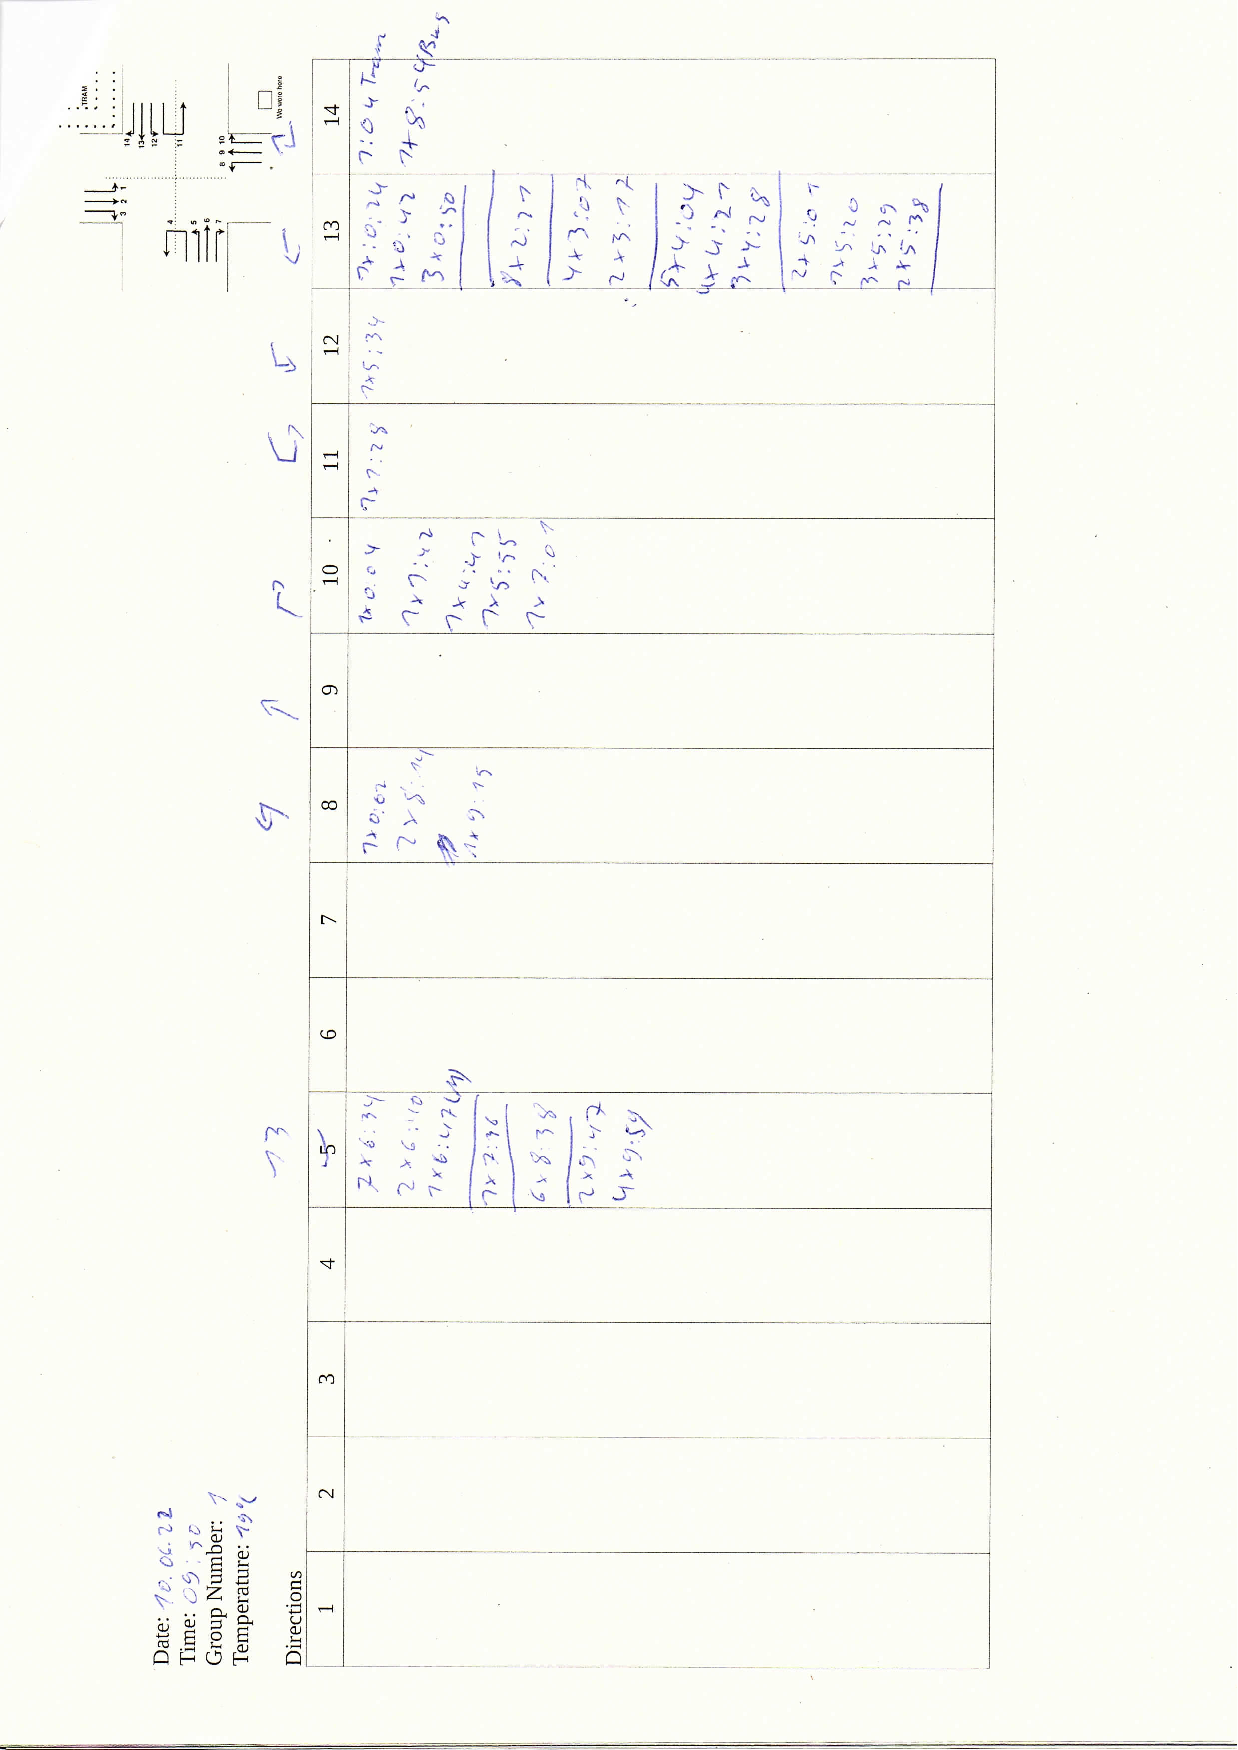
\includegraphics[width=\linewidth]{scans/100622_0950.pdf}
\end{figure*}

%\rotatebox{270}{\scalebox{.25}{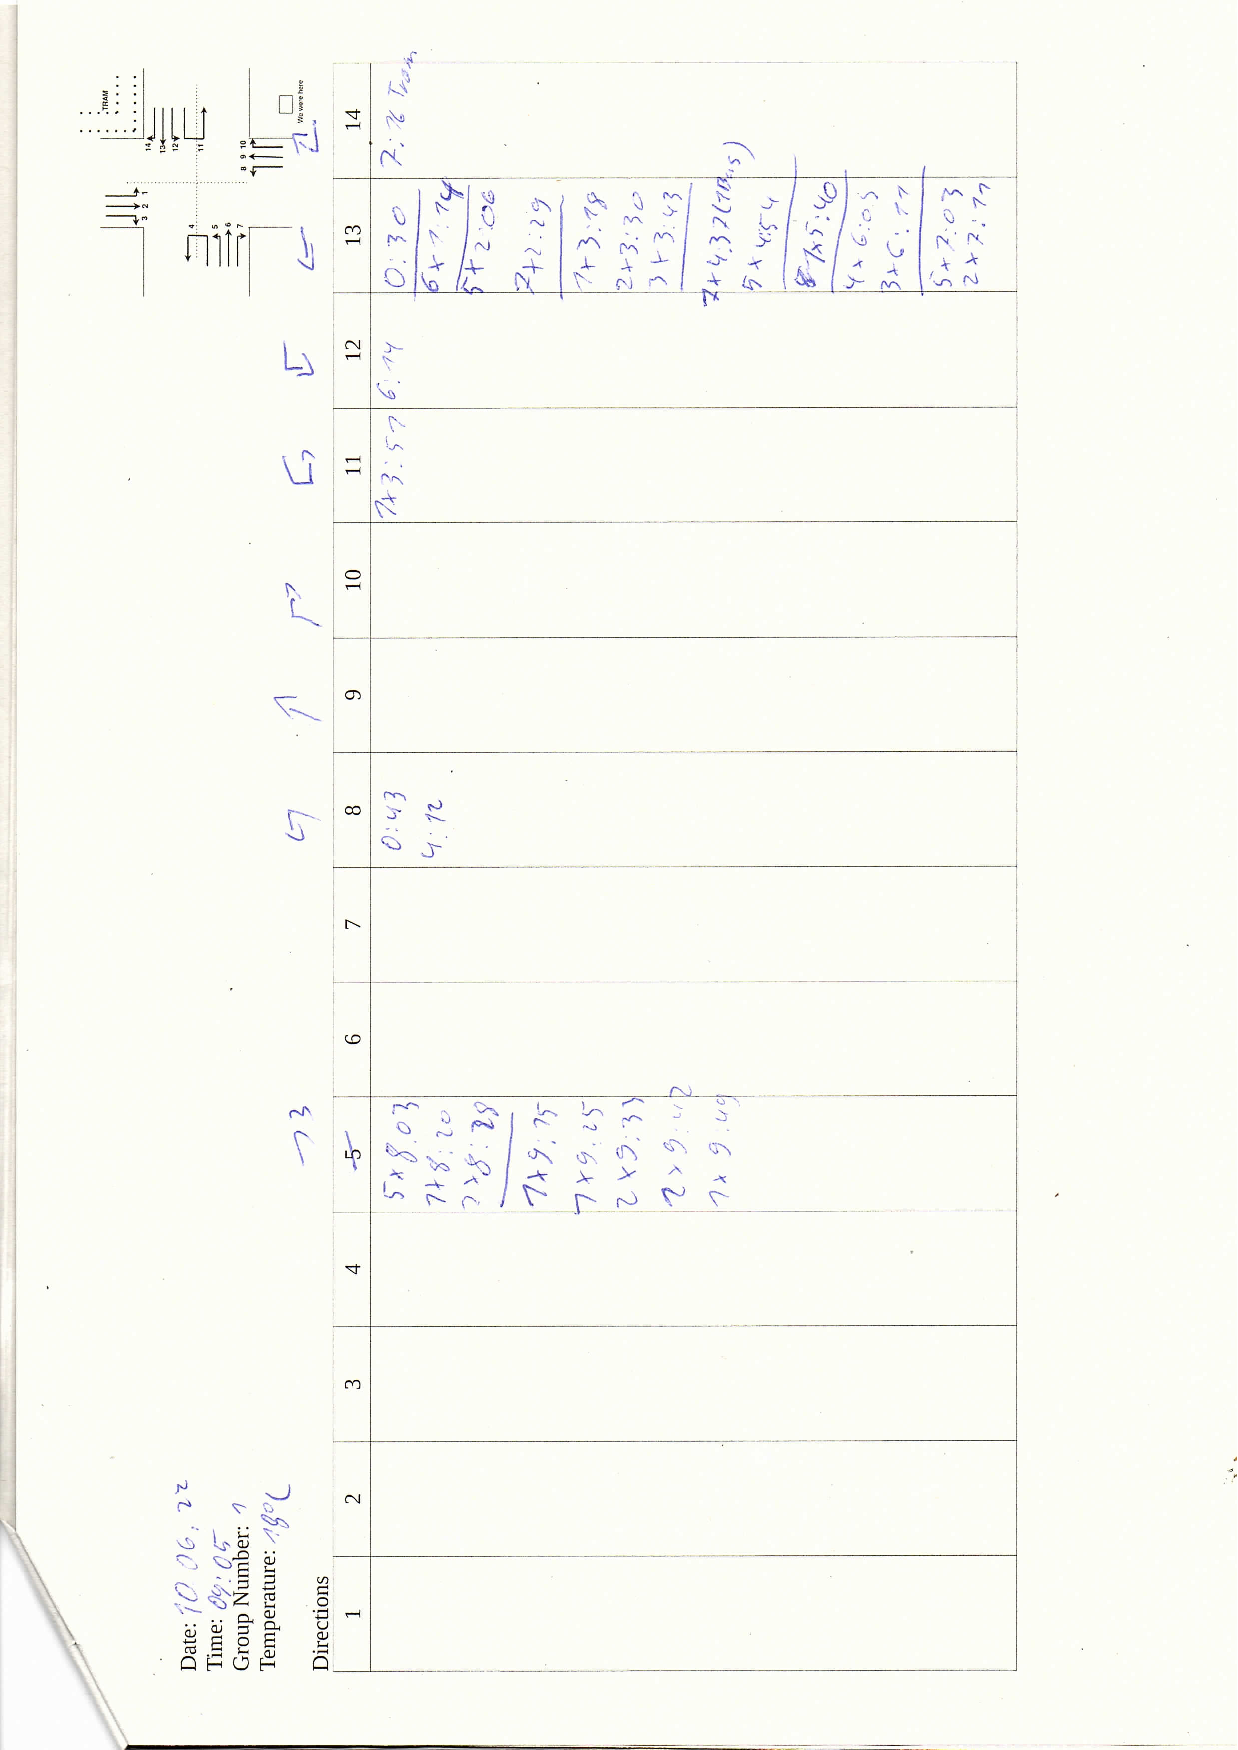
\includegraphics[]{scans/100622_0905.pdf}}}\\\\
%\rotatebox{270}{\scalebox{.25}{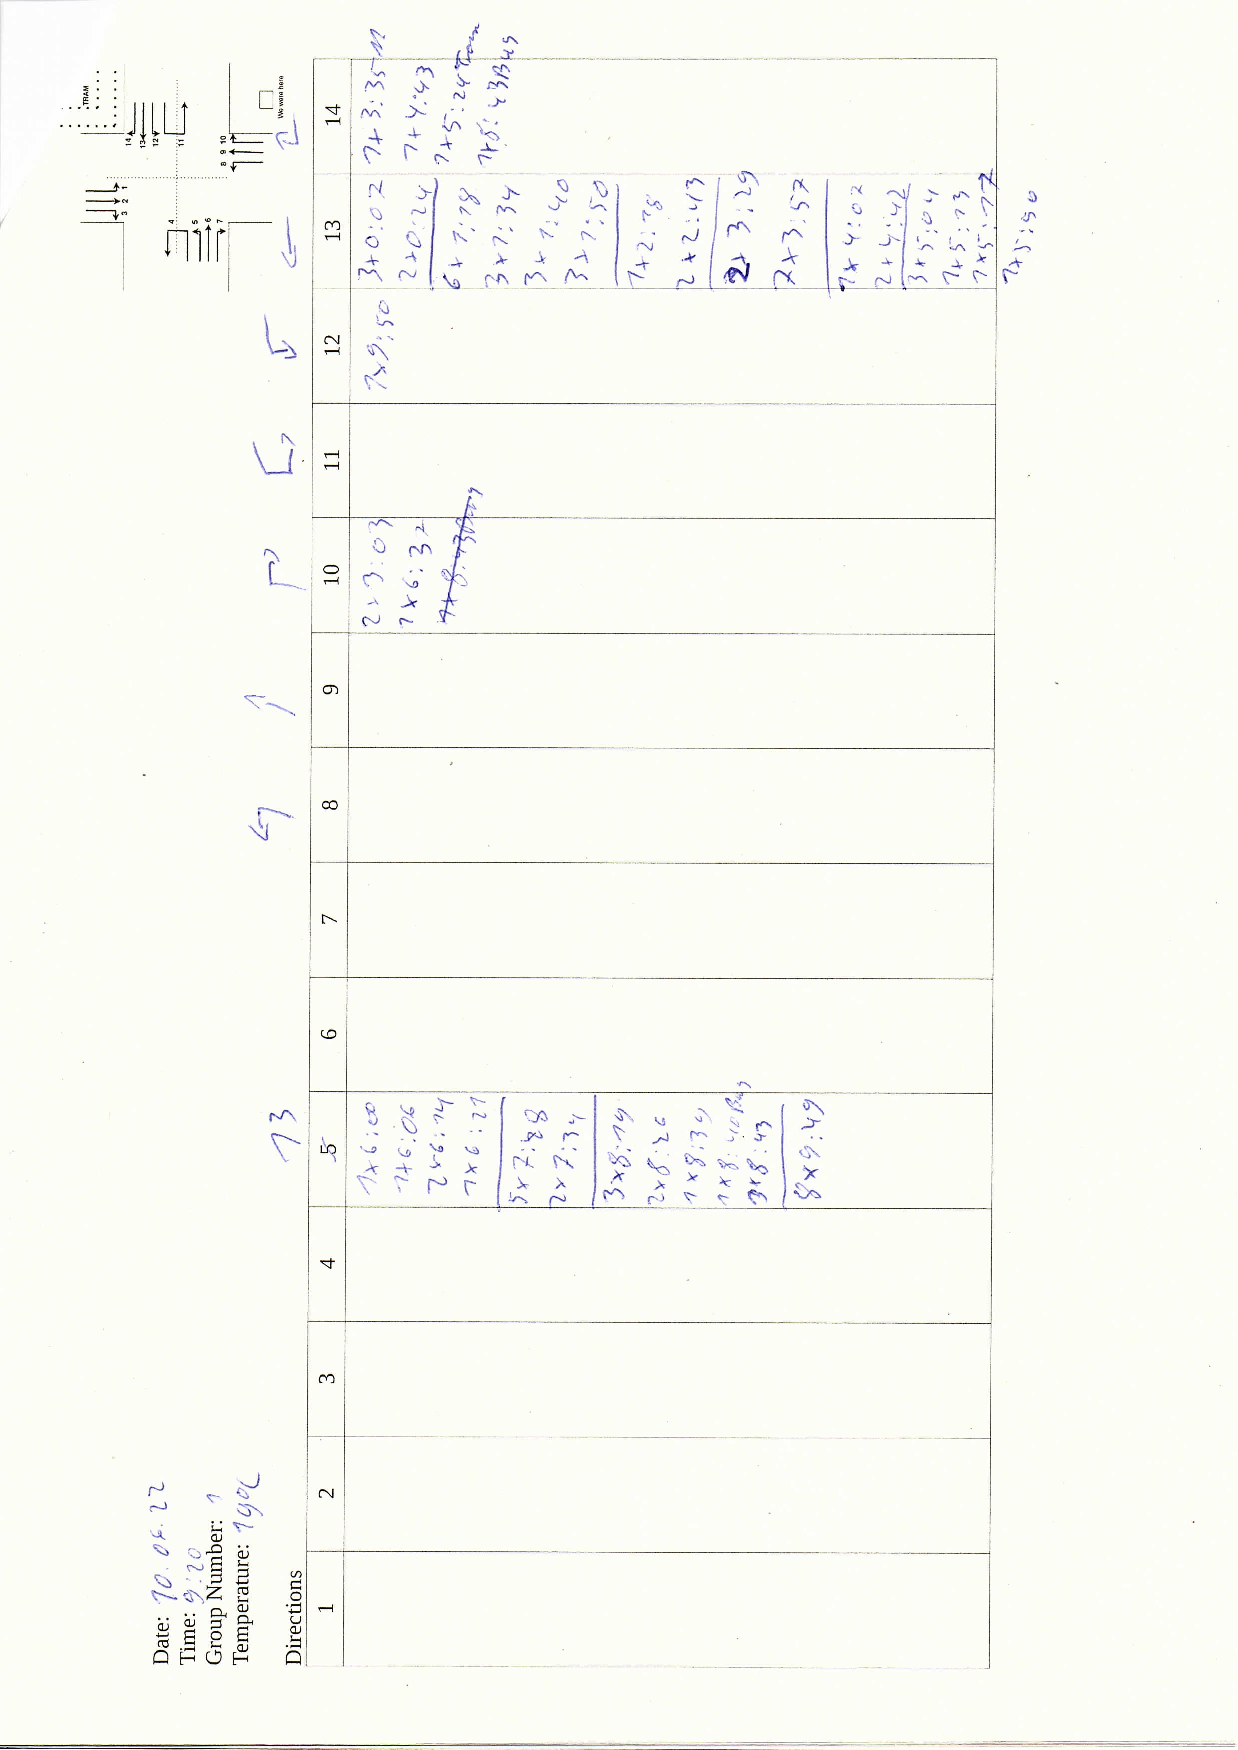
\includegraphics[]{scans/100622_0920.pdf}}}\\\\
%\rotatebox{270}{\scalebox{.25}{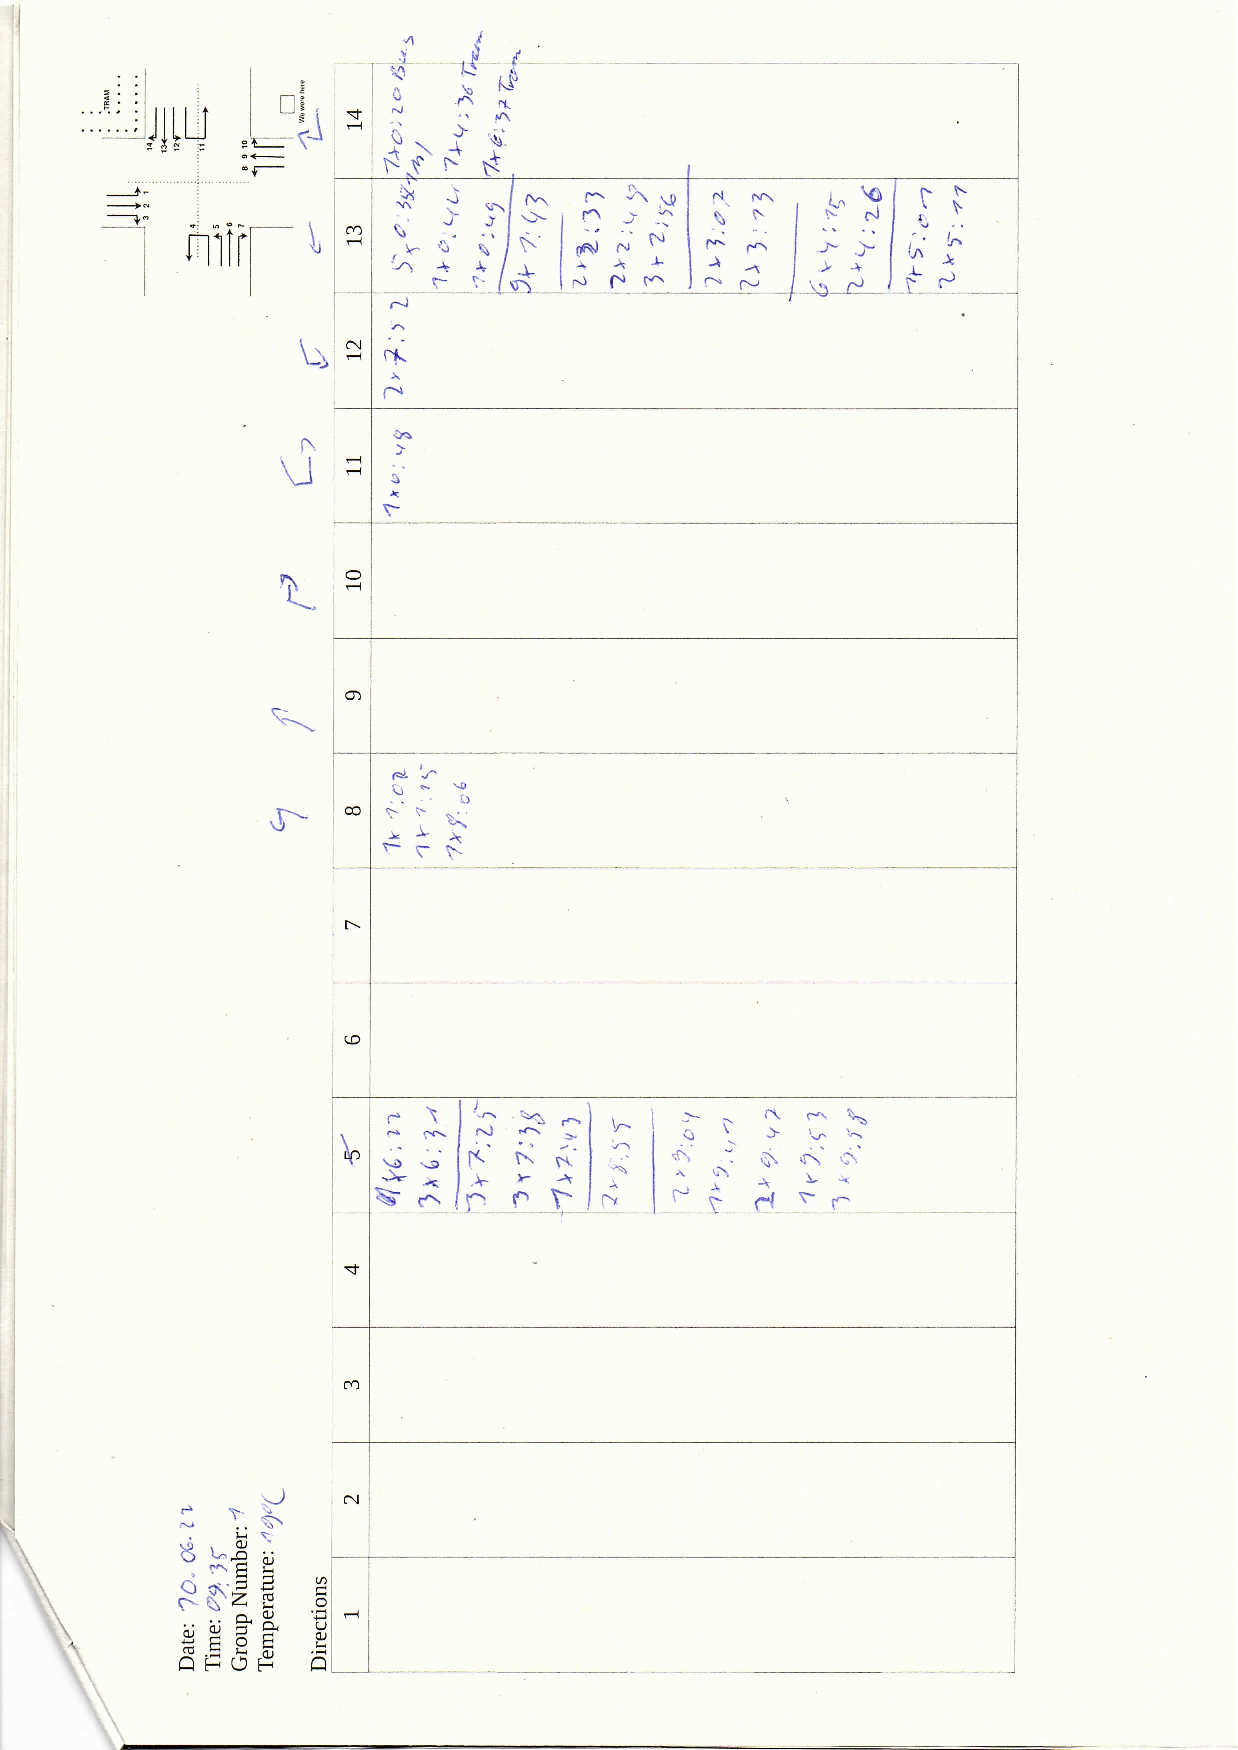
\includegraphics[]{scans/100622_0935.pdf}}}\\\\
%\rotatebox{270}{\scalebox{.25}{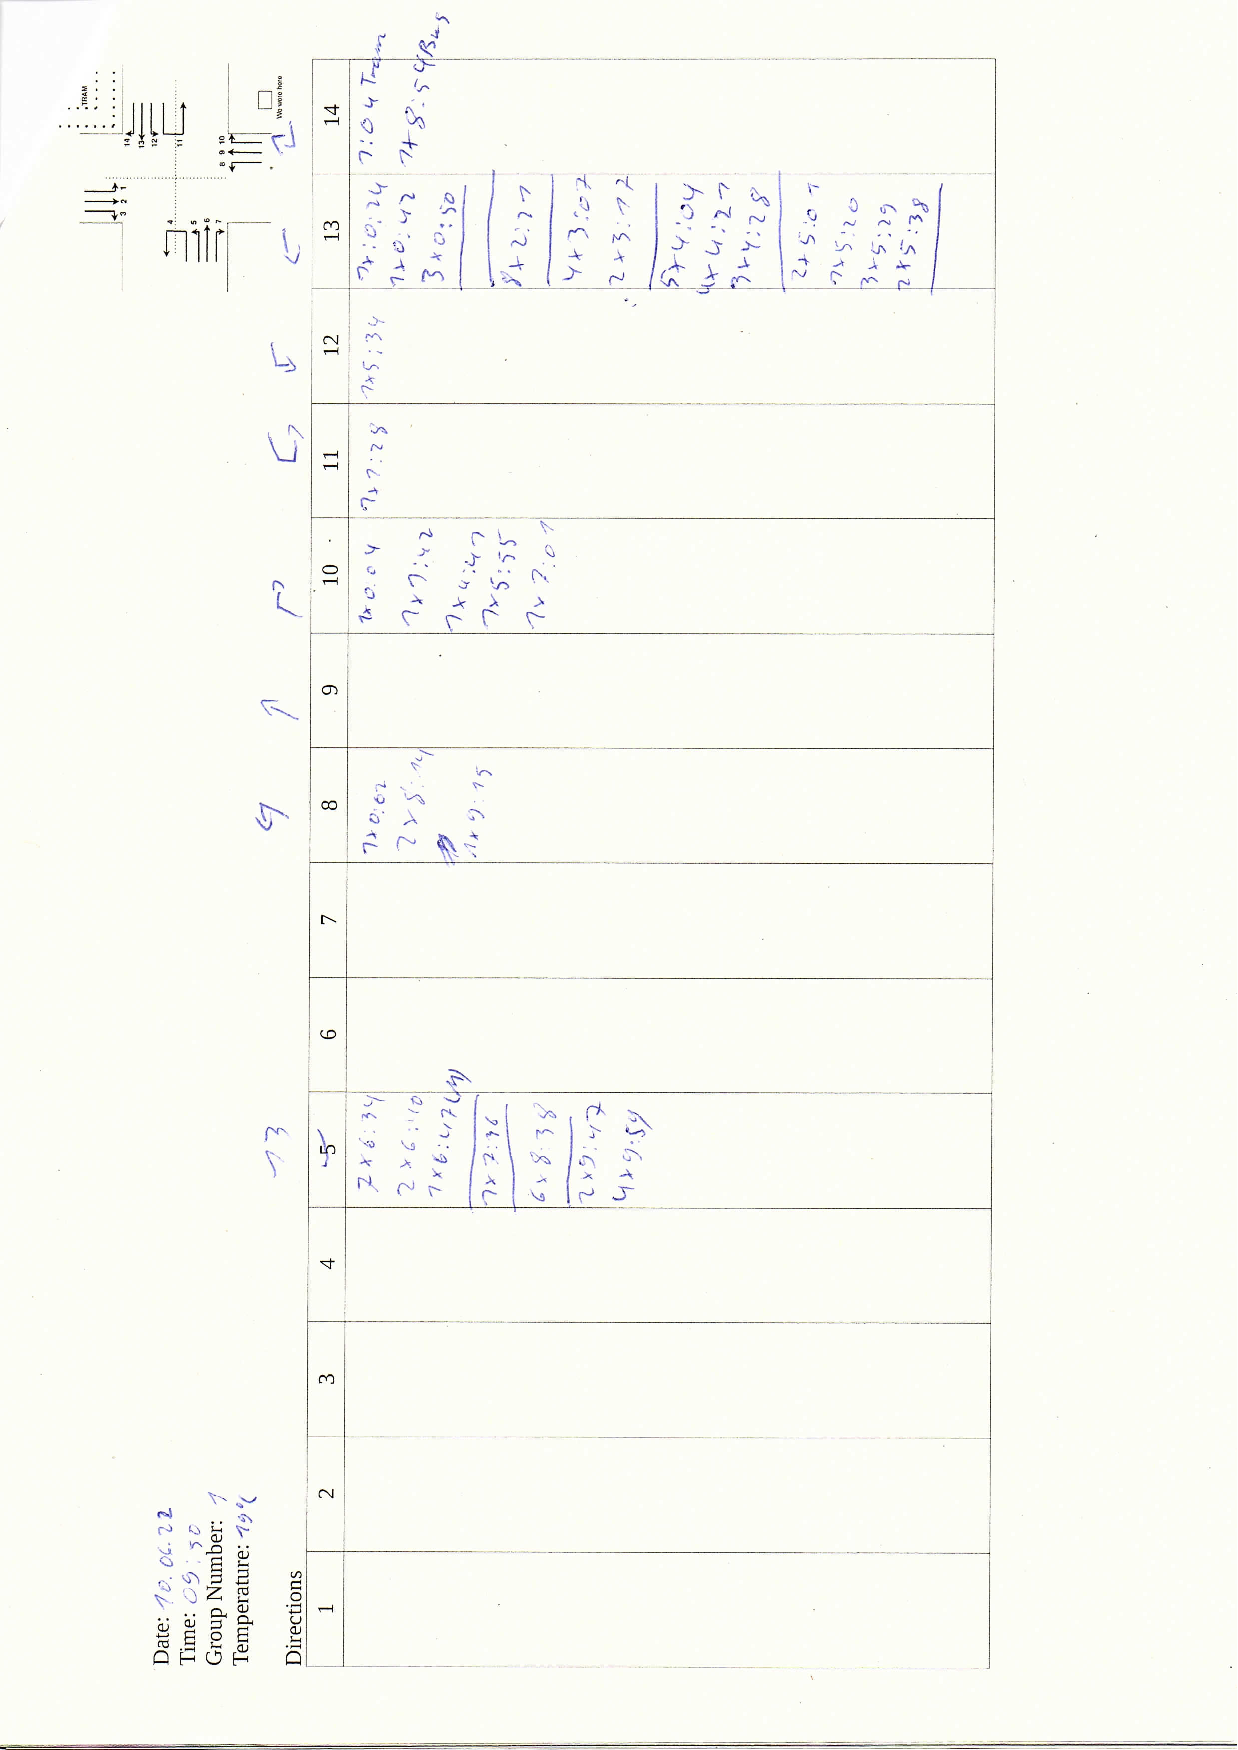
\includegraphics[]{scans/100622_0950.pdf}}}\\\\

\begin{figure*}[htbp]
  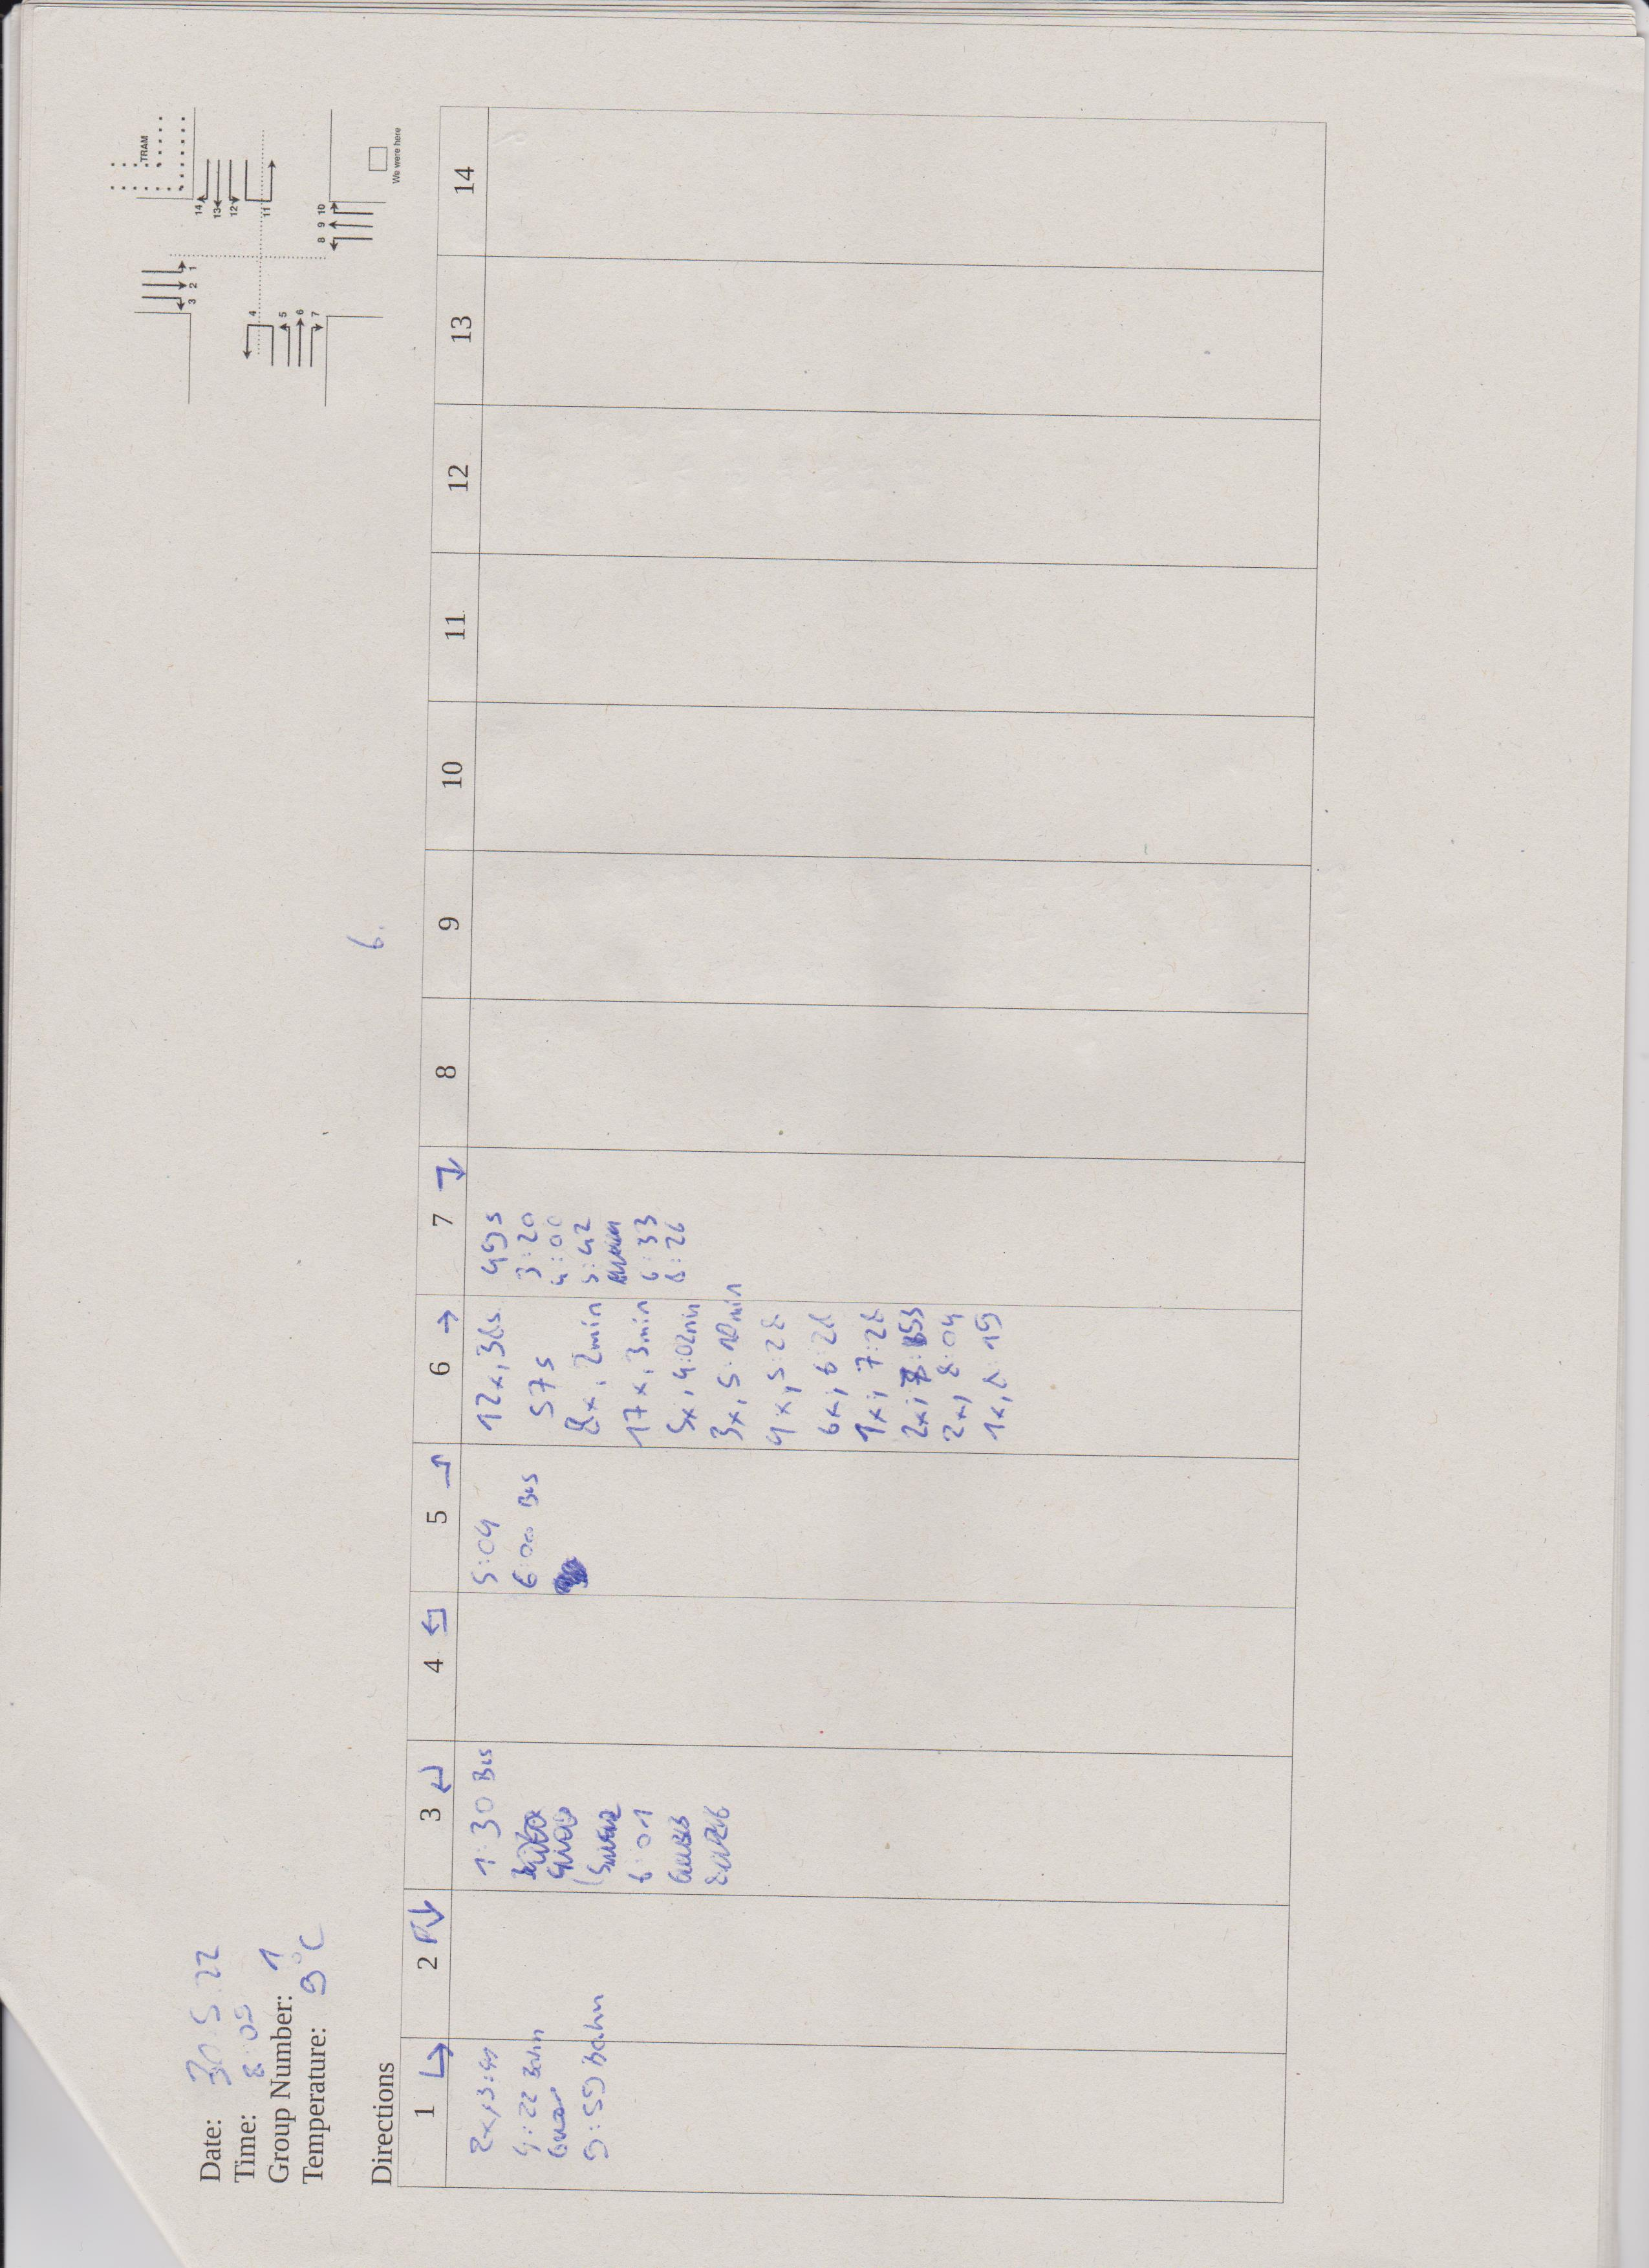
\includegraphics[width=\linewidth]{scans/Bild (1).jpg}
\end{figure*}

\begin{figure*}[htbp]
  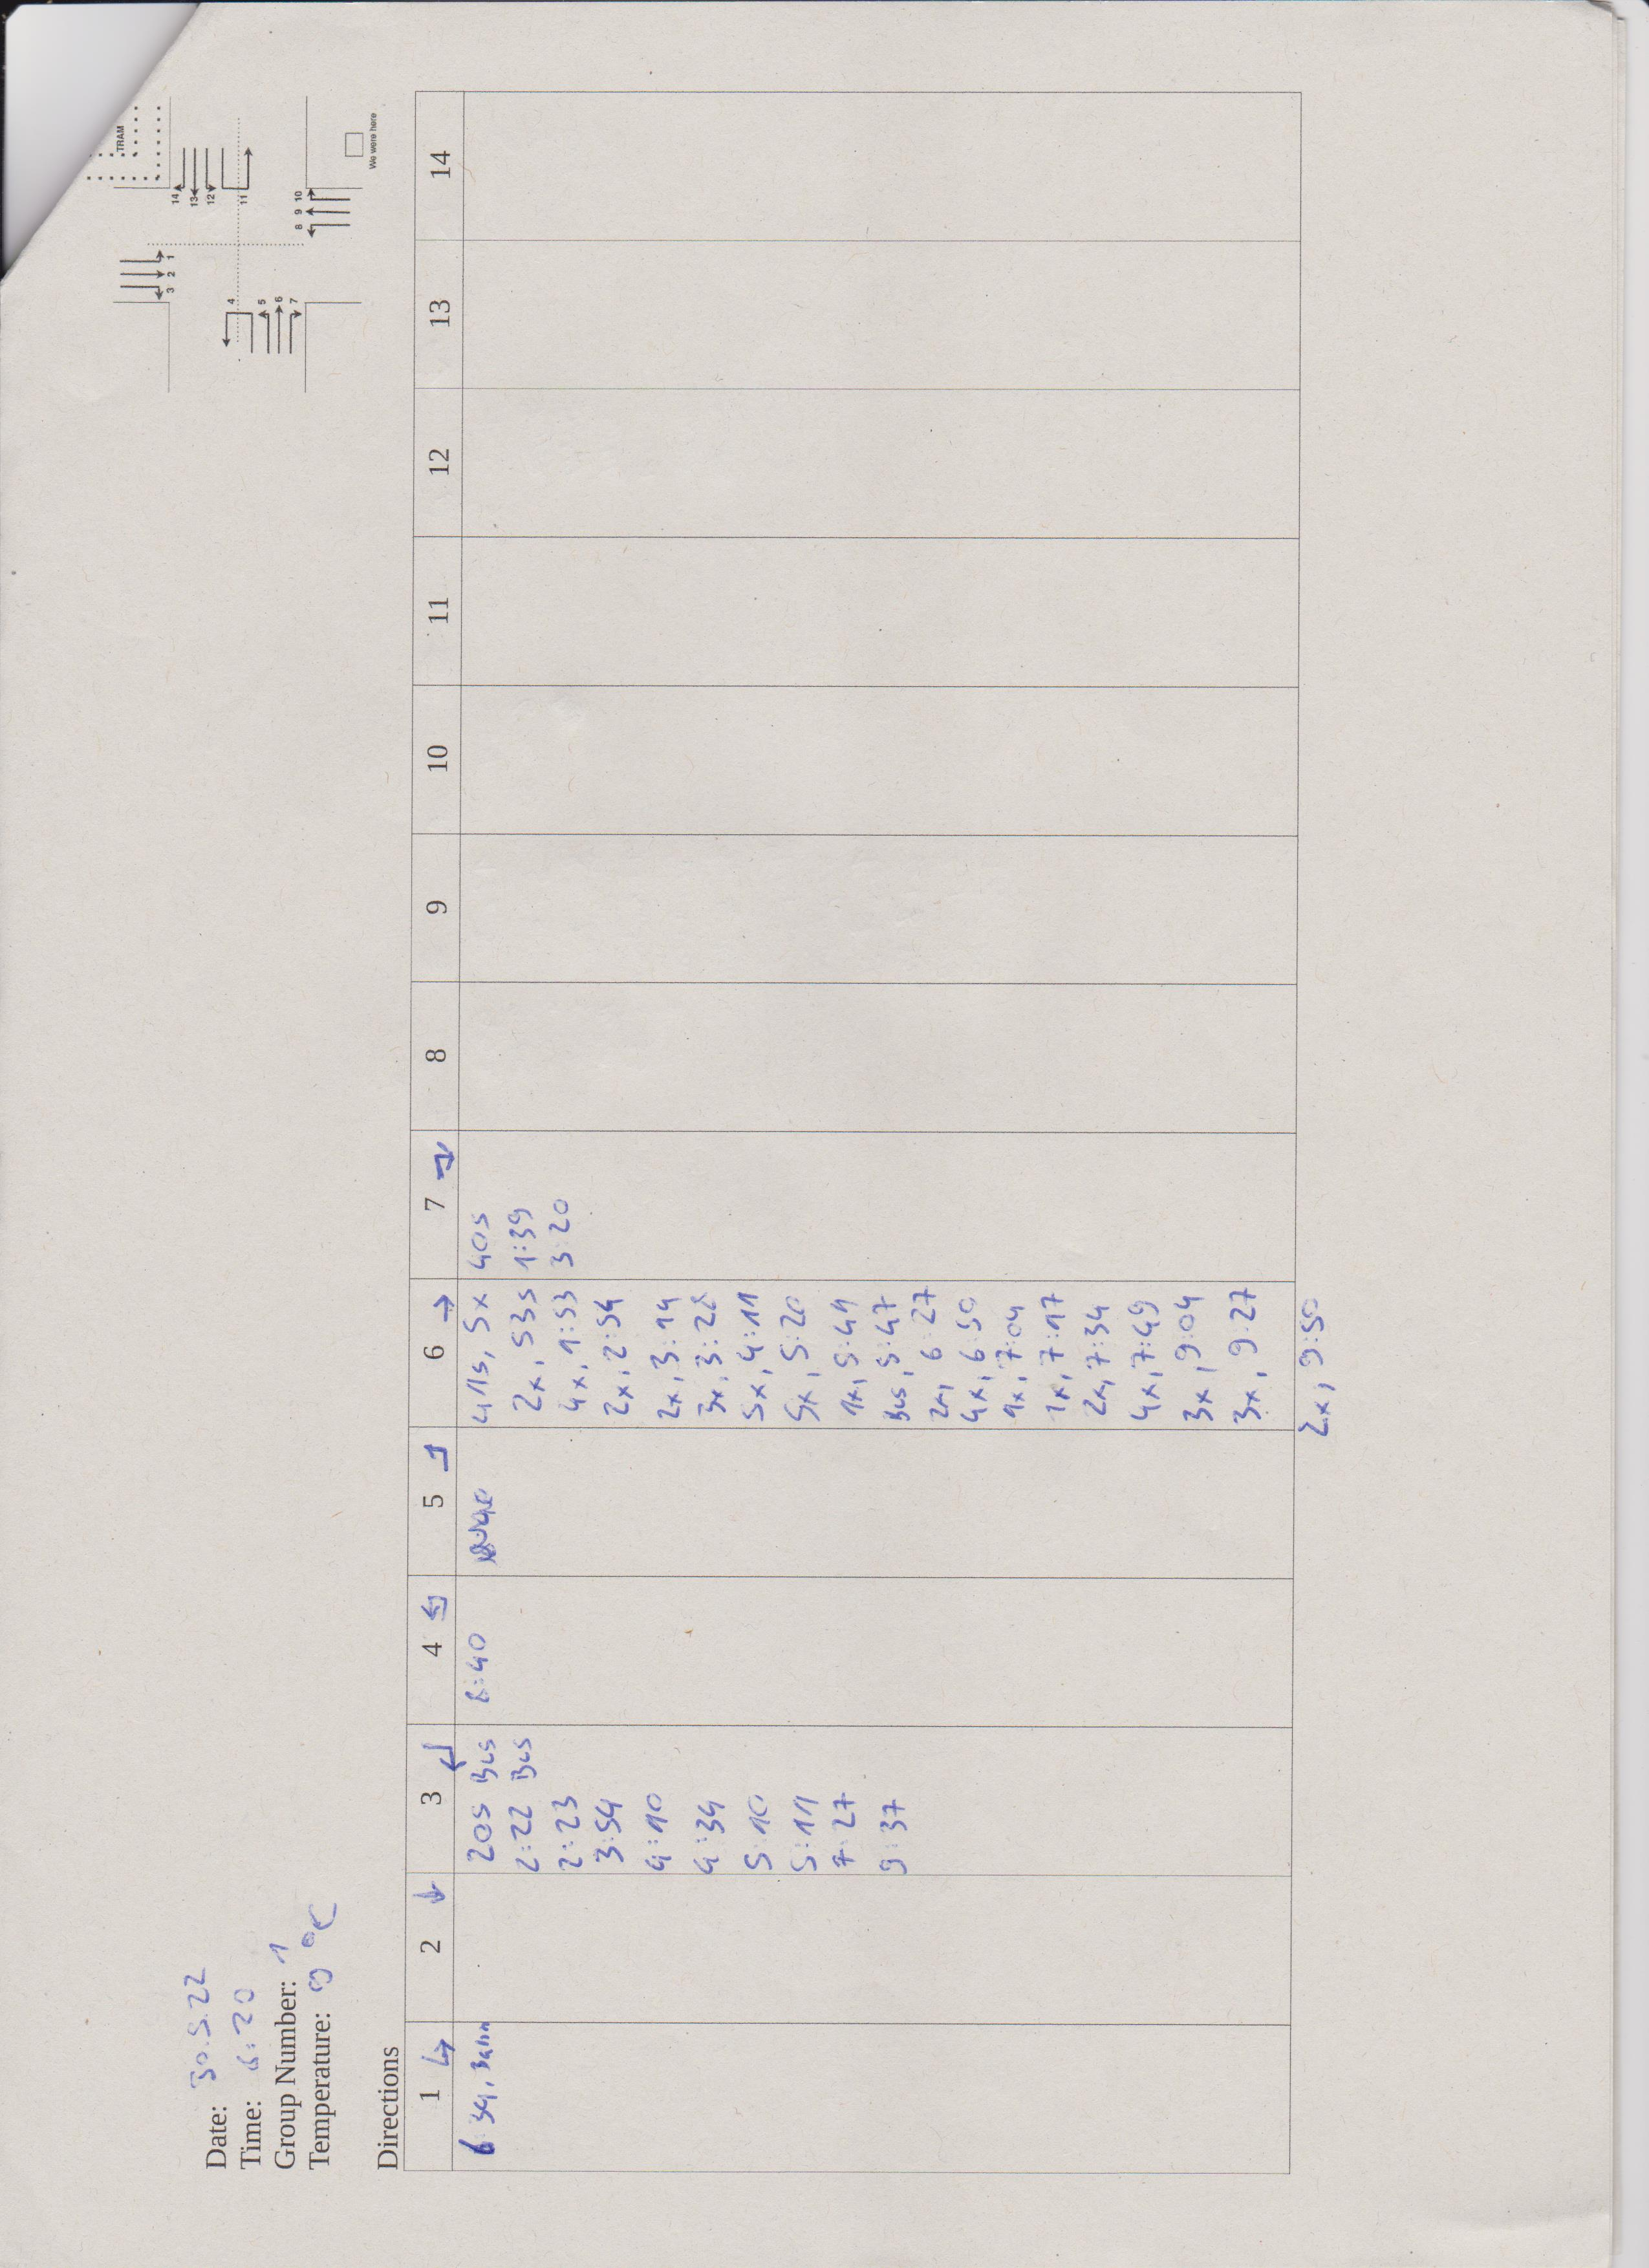
\includegraphics[width=\linewidth]{scans/Bild (2).jpg})
\end{figure*}

\begin{figure*}[htbp]
  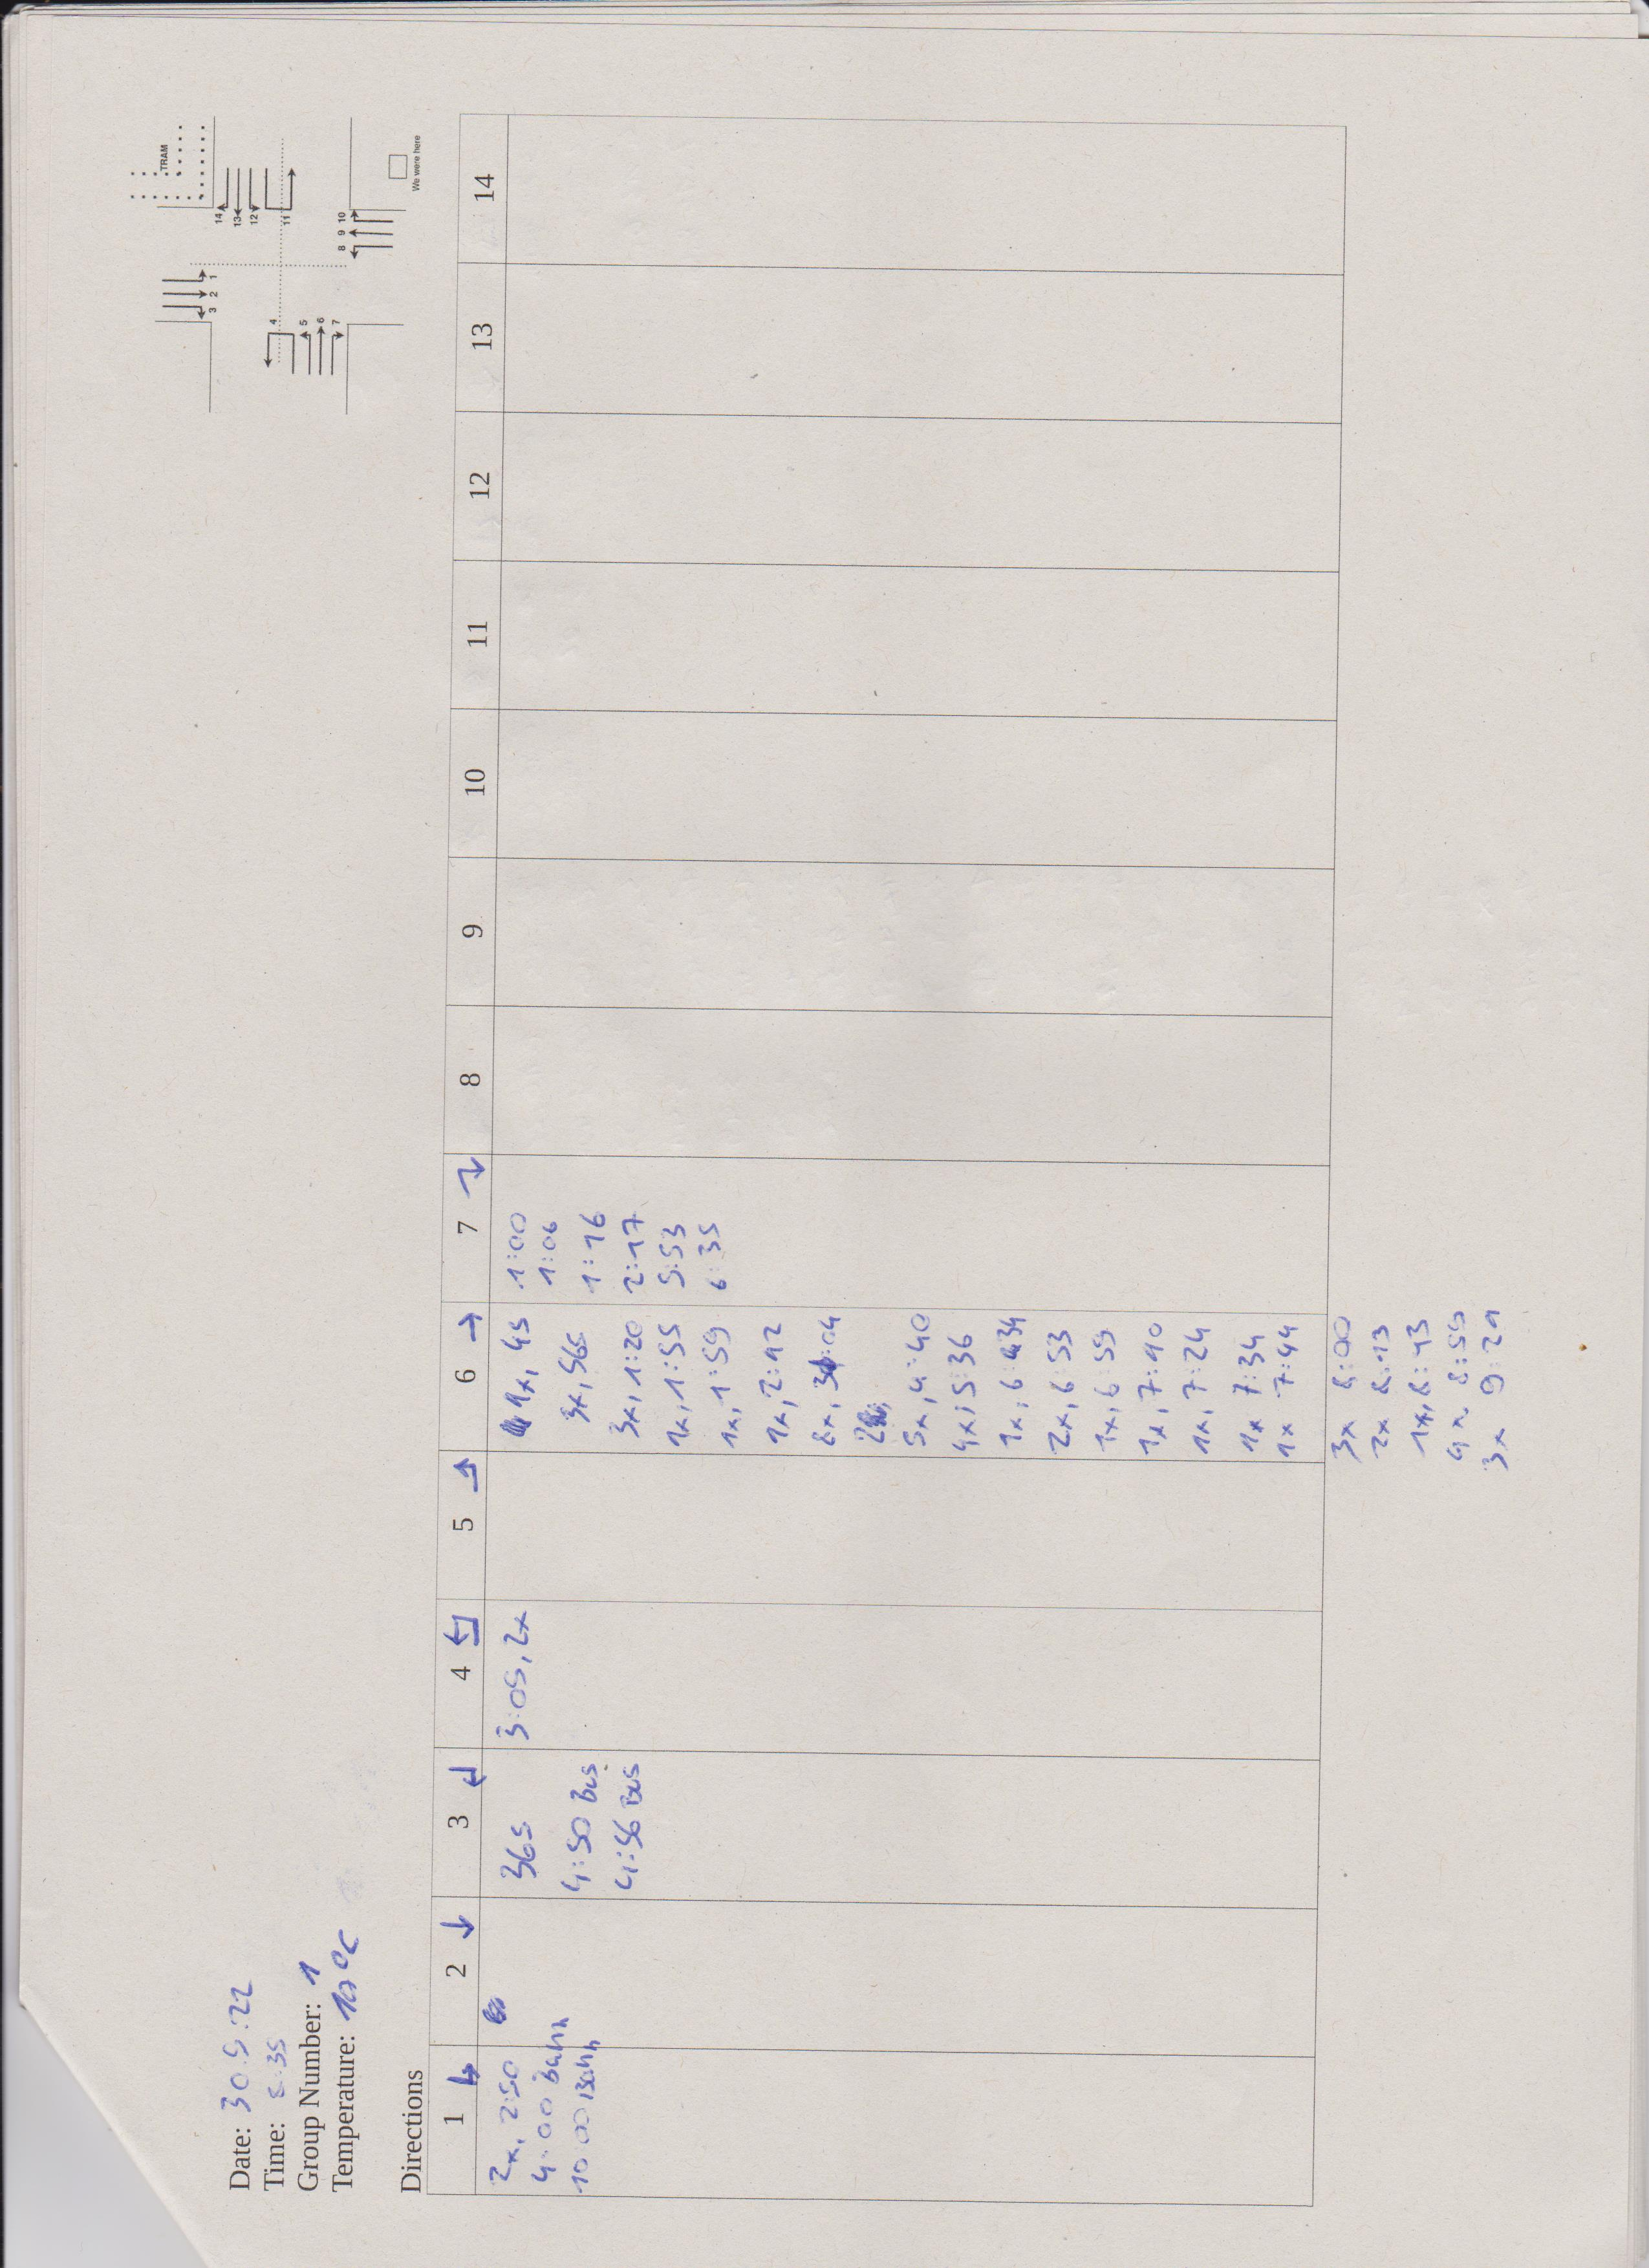
\includegraphics[width=\linewidth]{scans/Bild (3).jpg}
\end{figure*}

\begin{figure*}[htbp]
  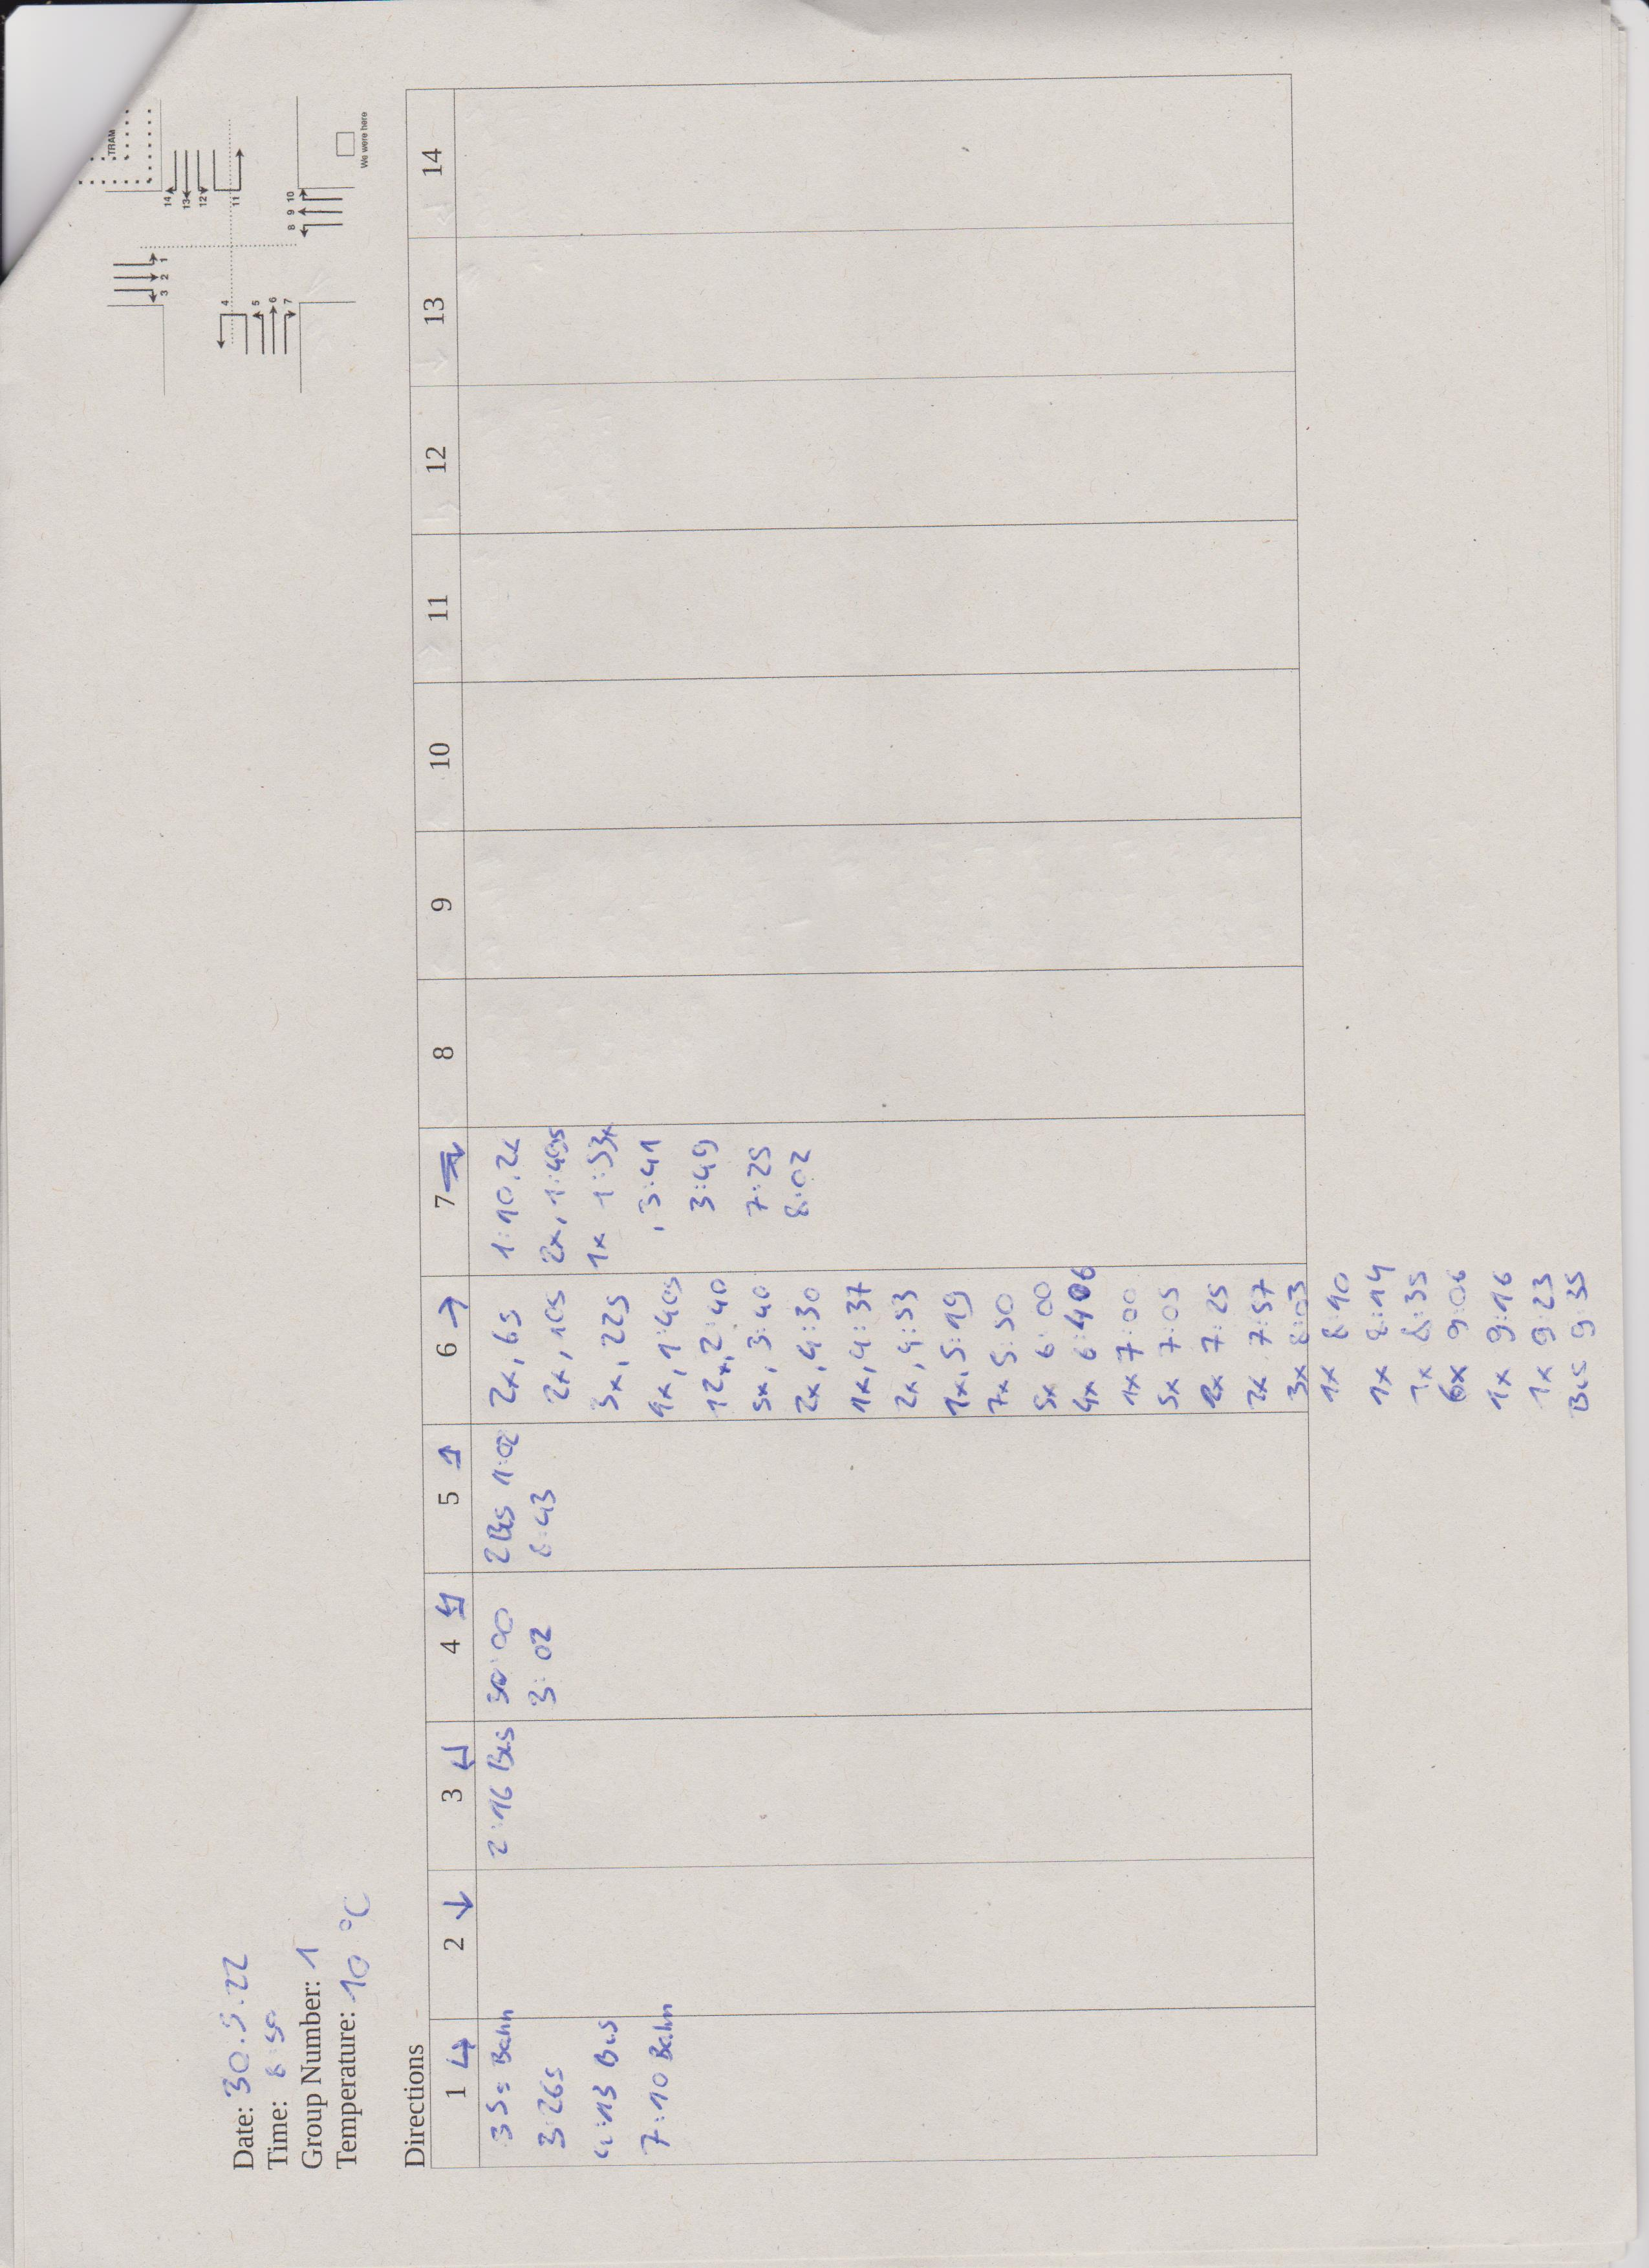
\includegraphics[width=\linewidth]{scans/Bild (4).jpg}
\end{figure*}

\begin{figure*}[htbp]
  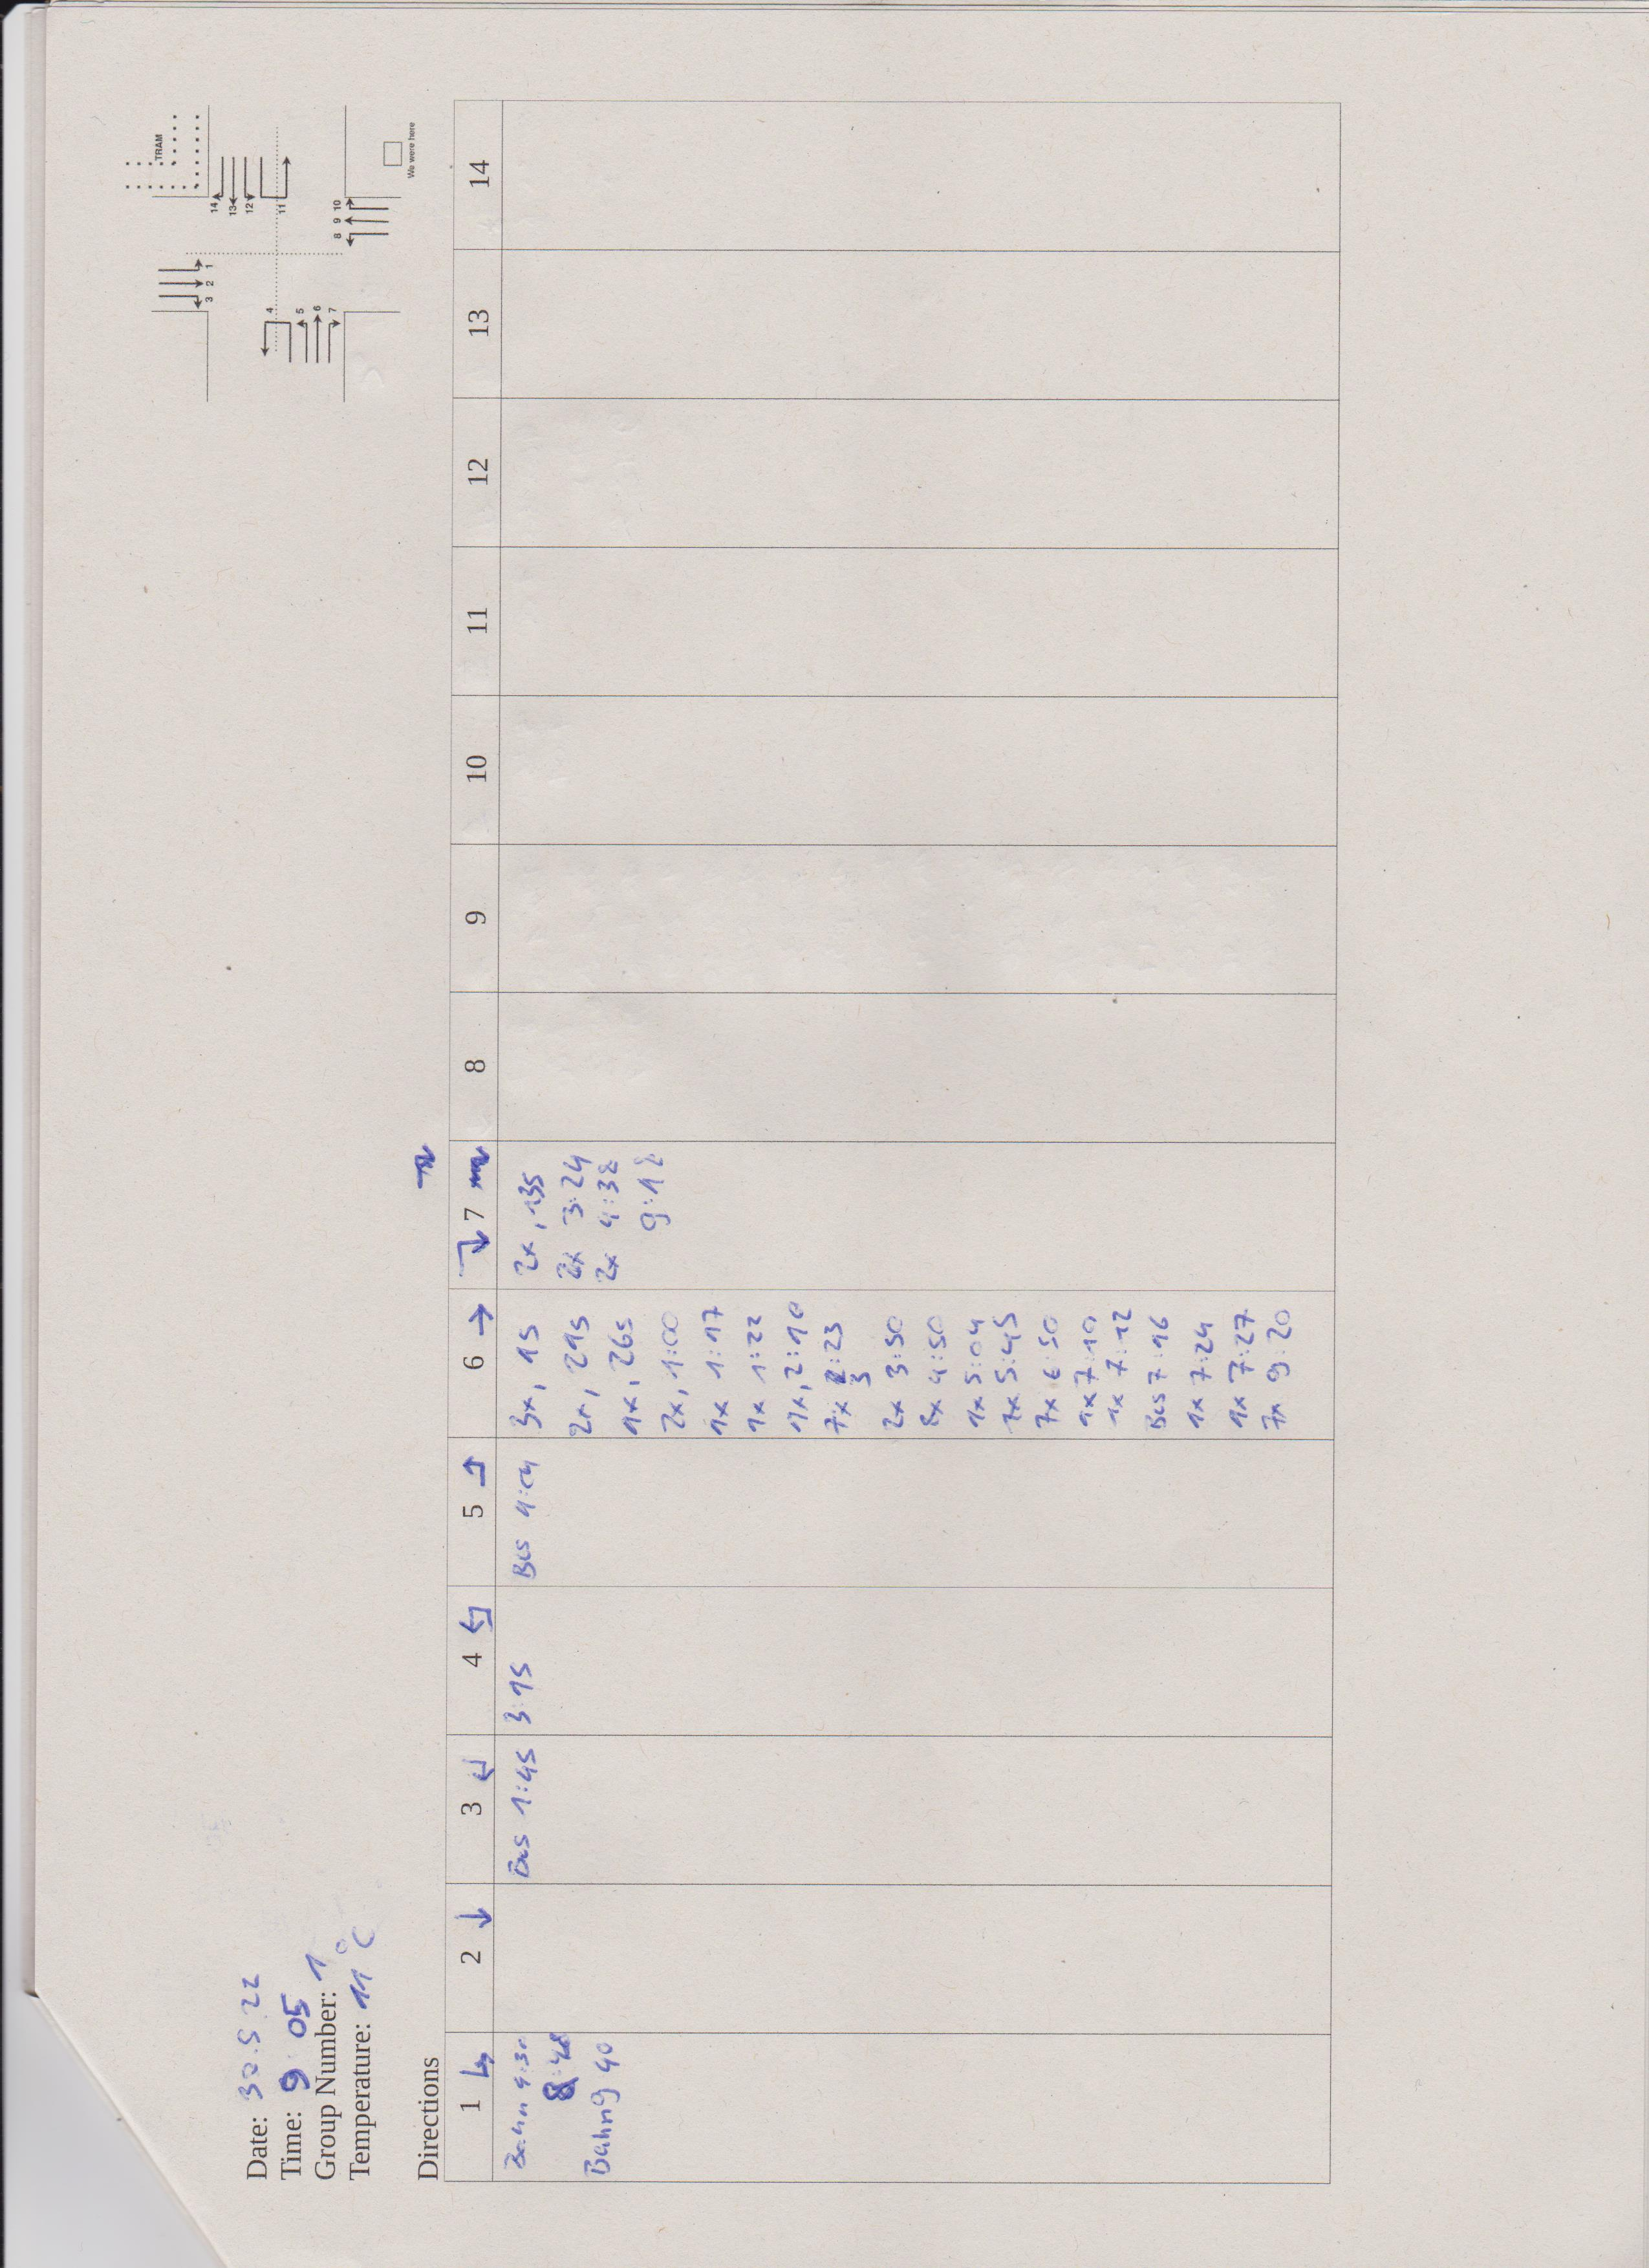
\includegraphics[width=\linewidth]{scans/Bild (5).jpg}
\end{figure*}

\begin{figure*}[htbp]
  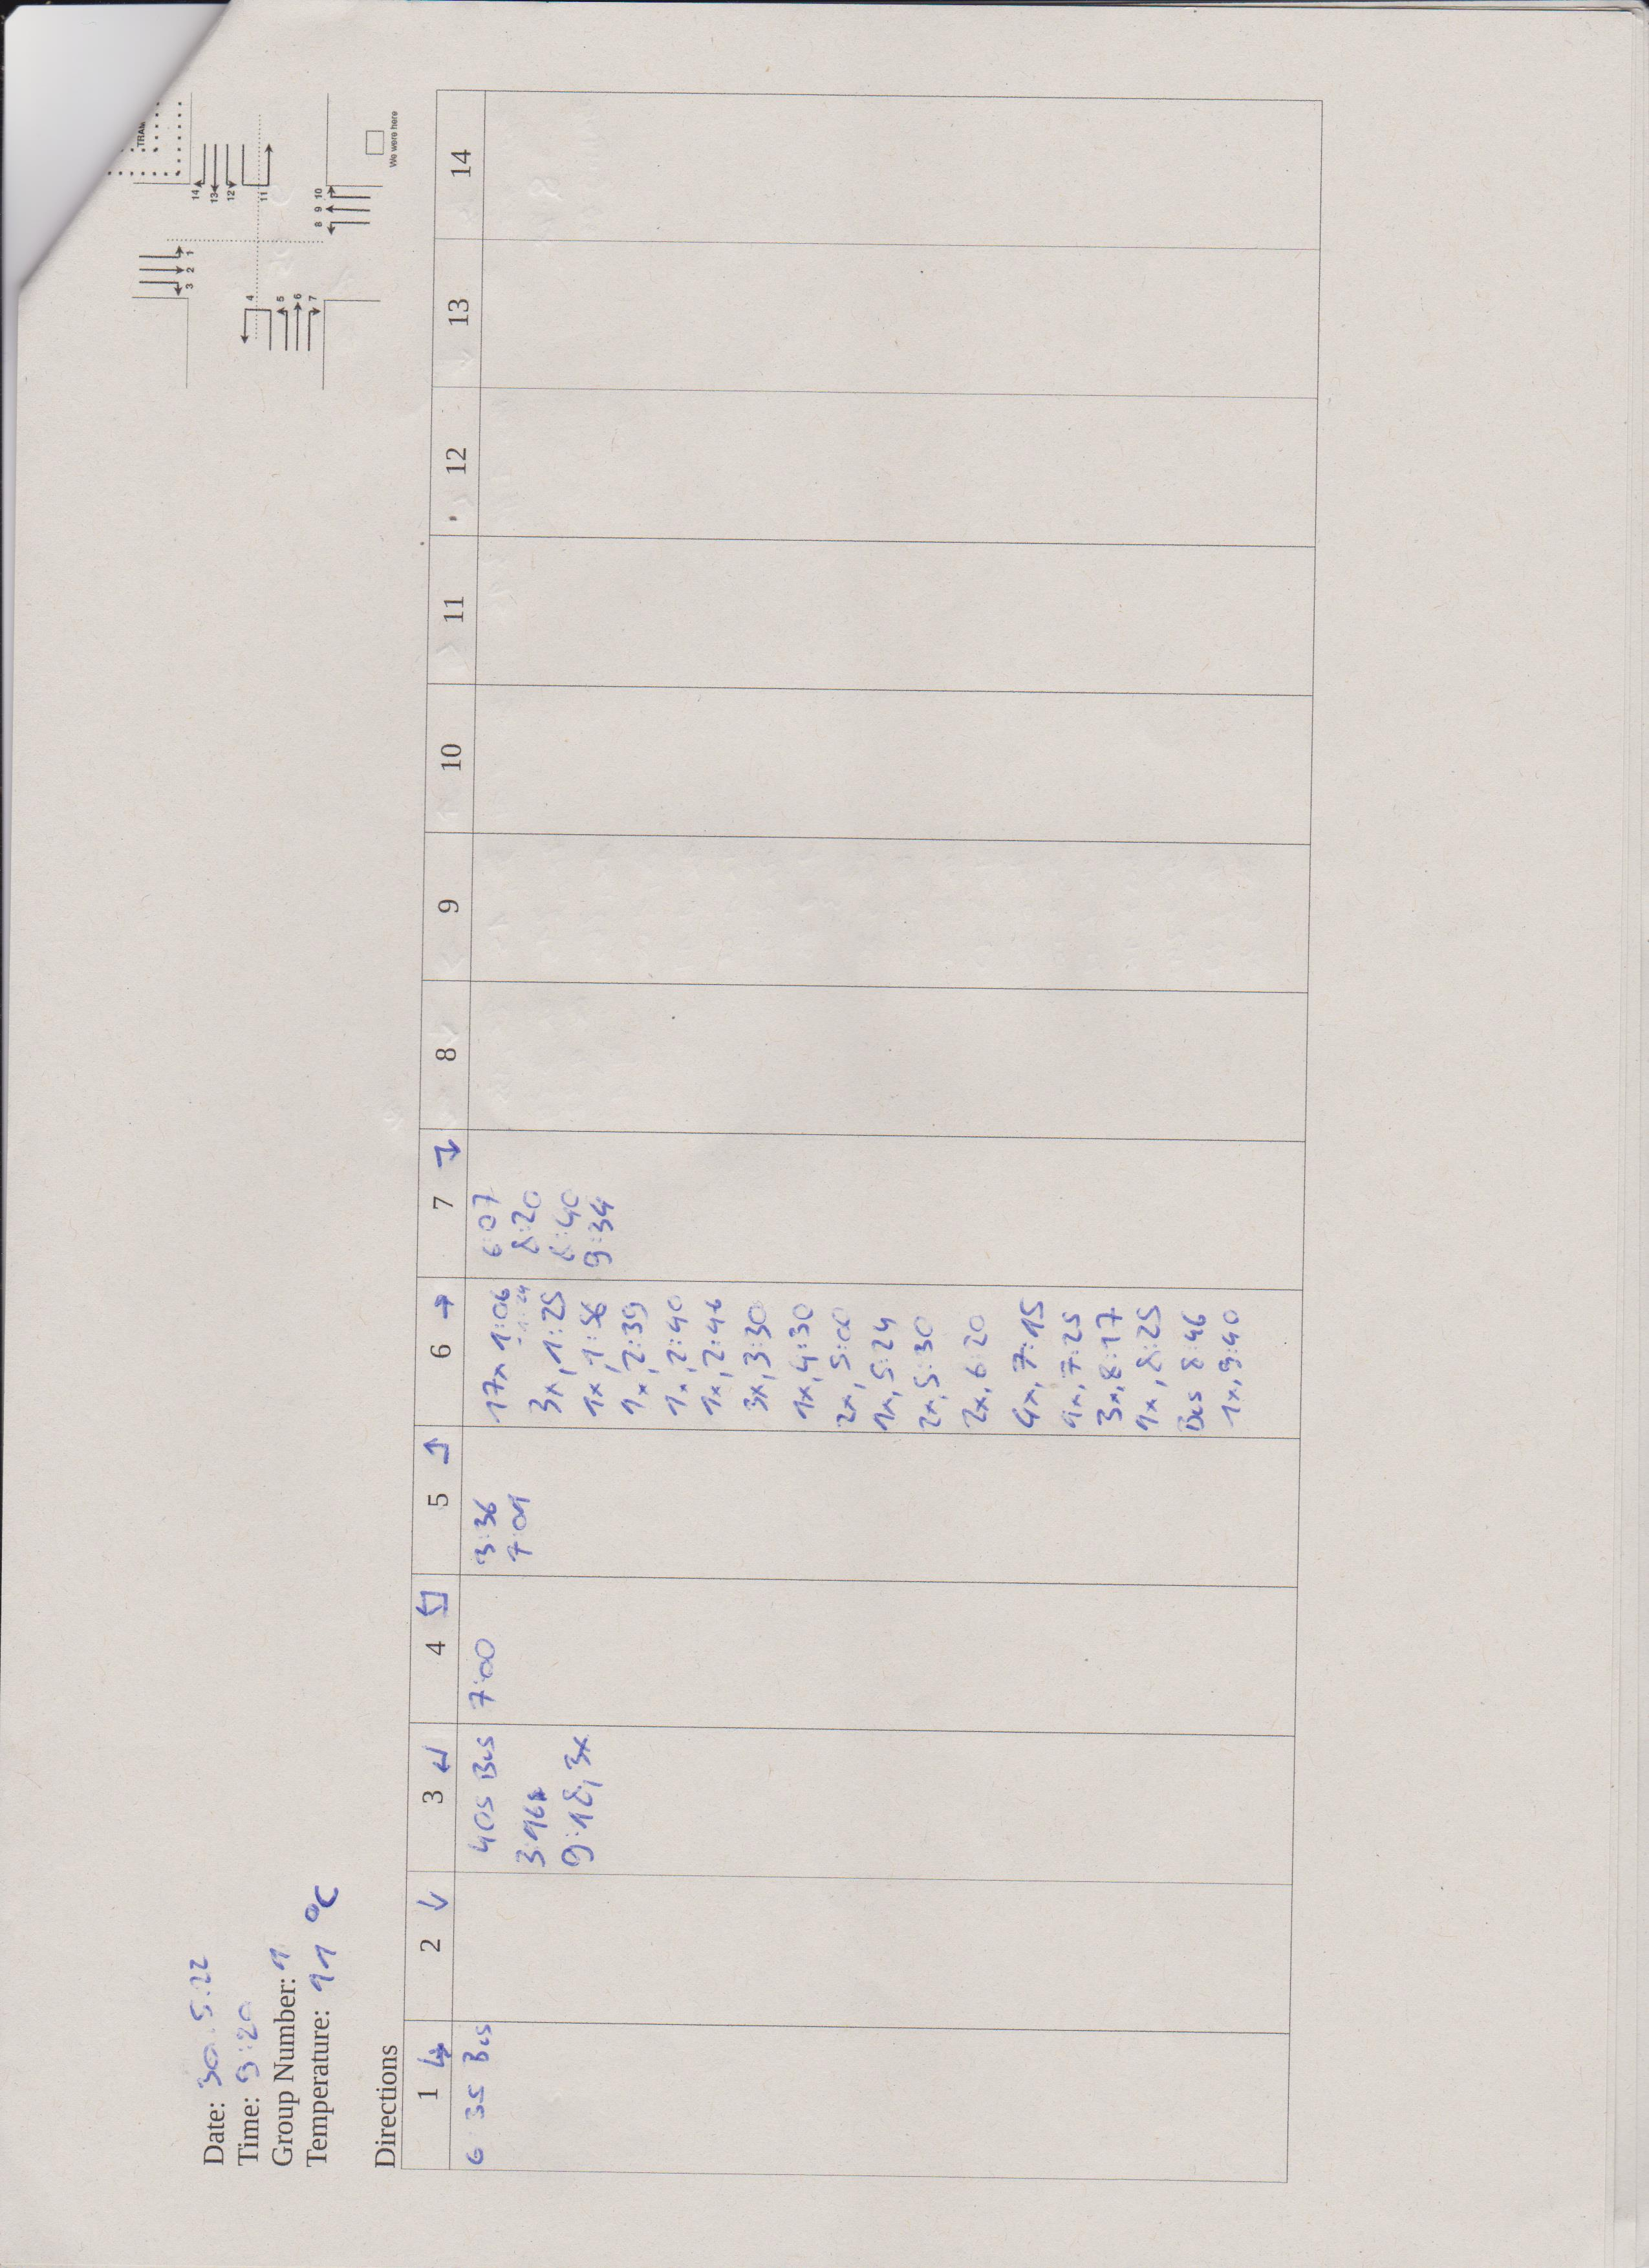
\includegraphics[width=\linewidth]{scans/Bild (6).jpg}
\end{figure*}

\begin{figure*}[htbp]
  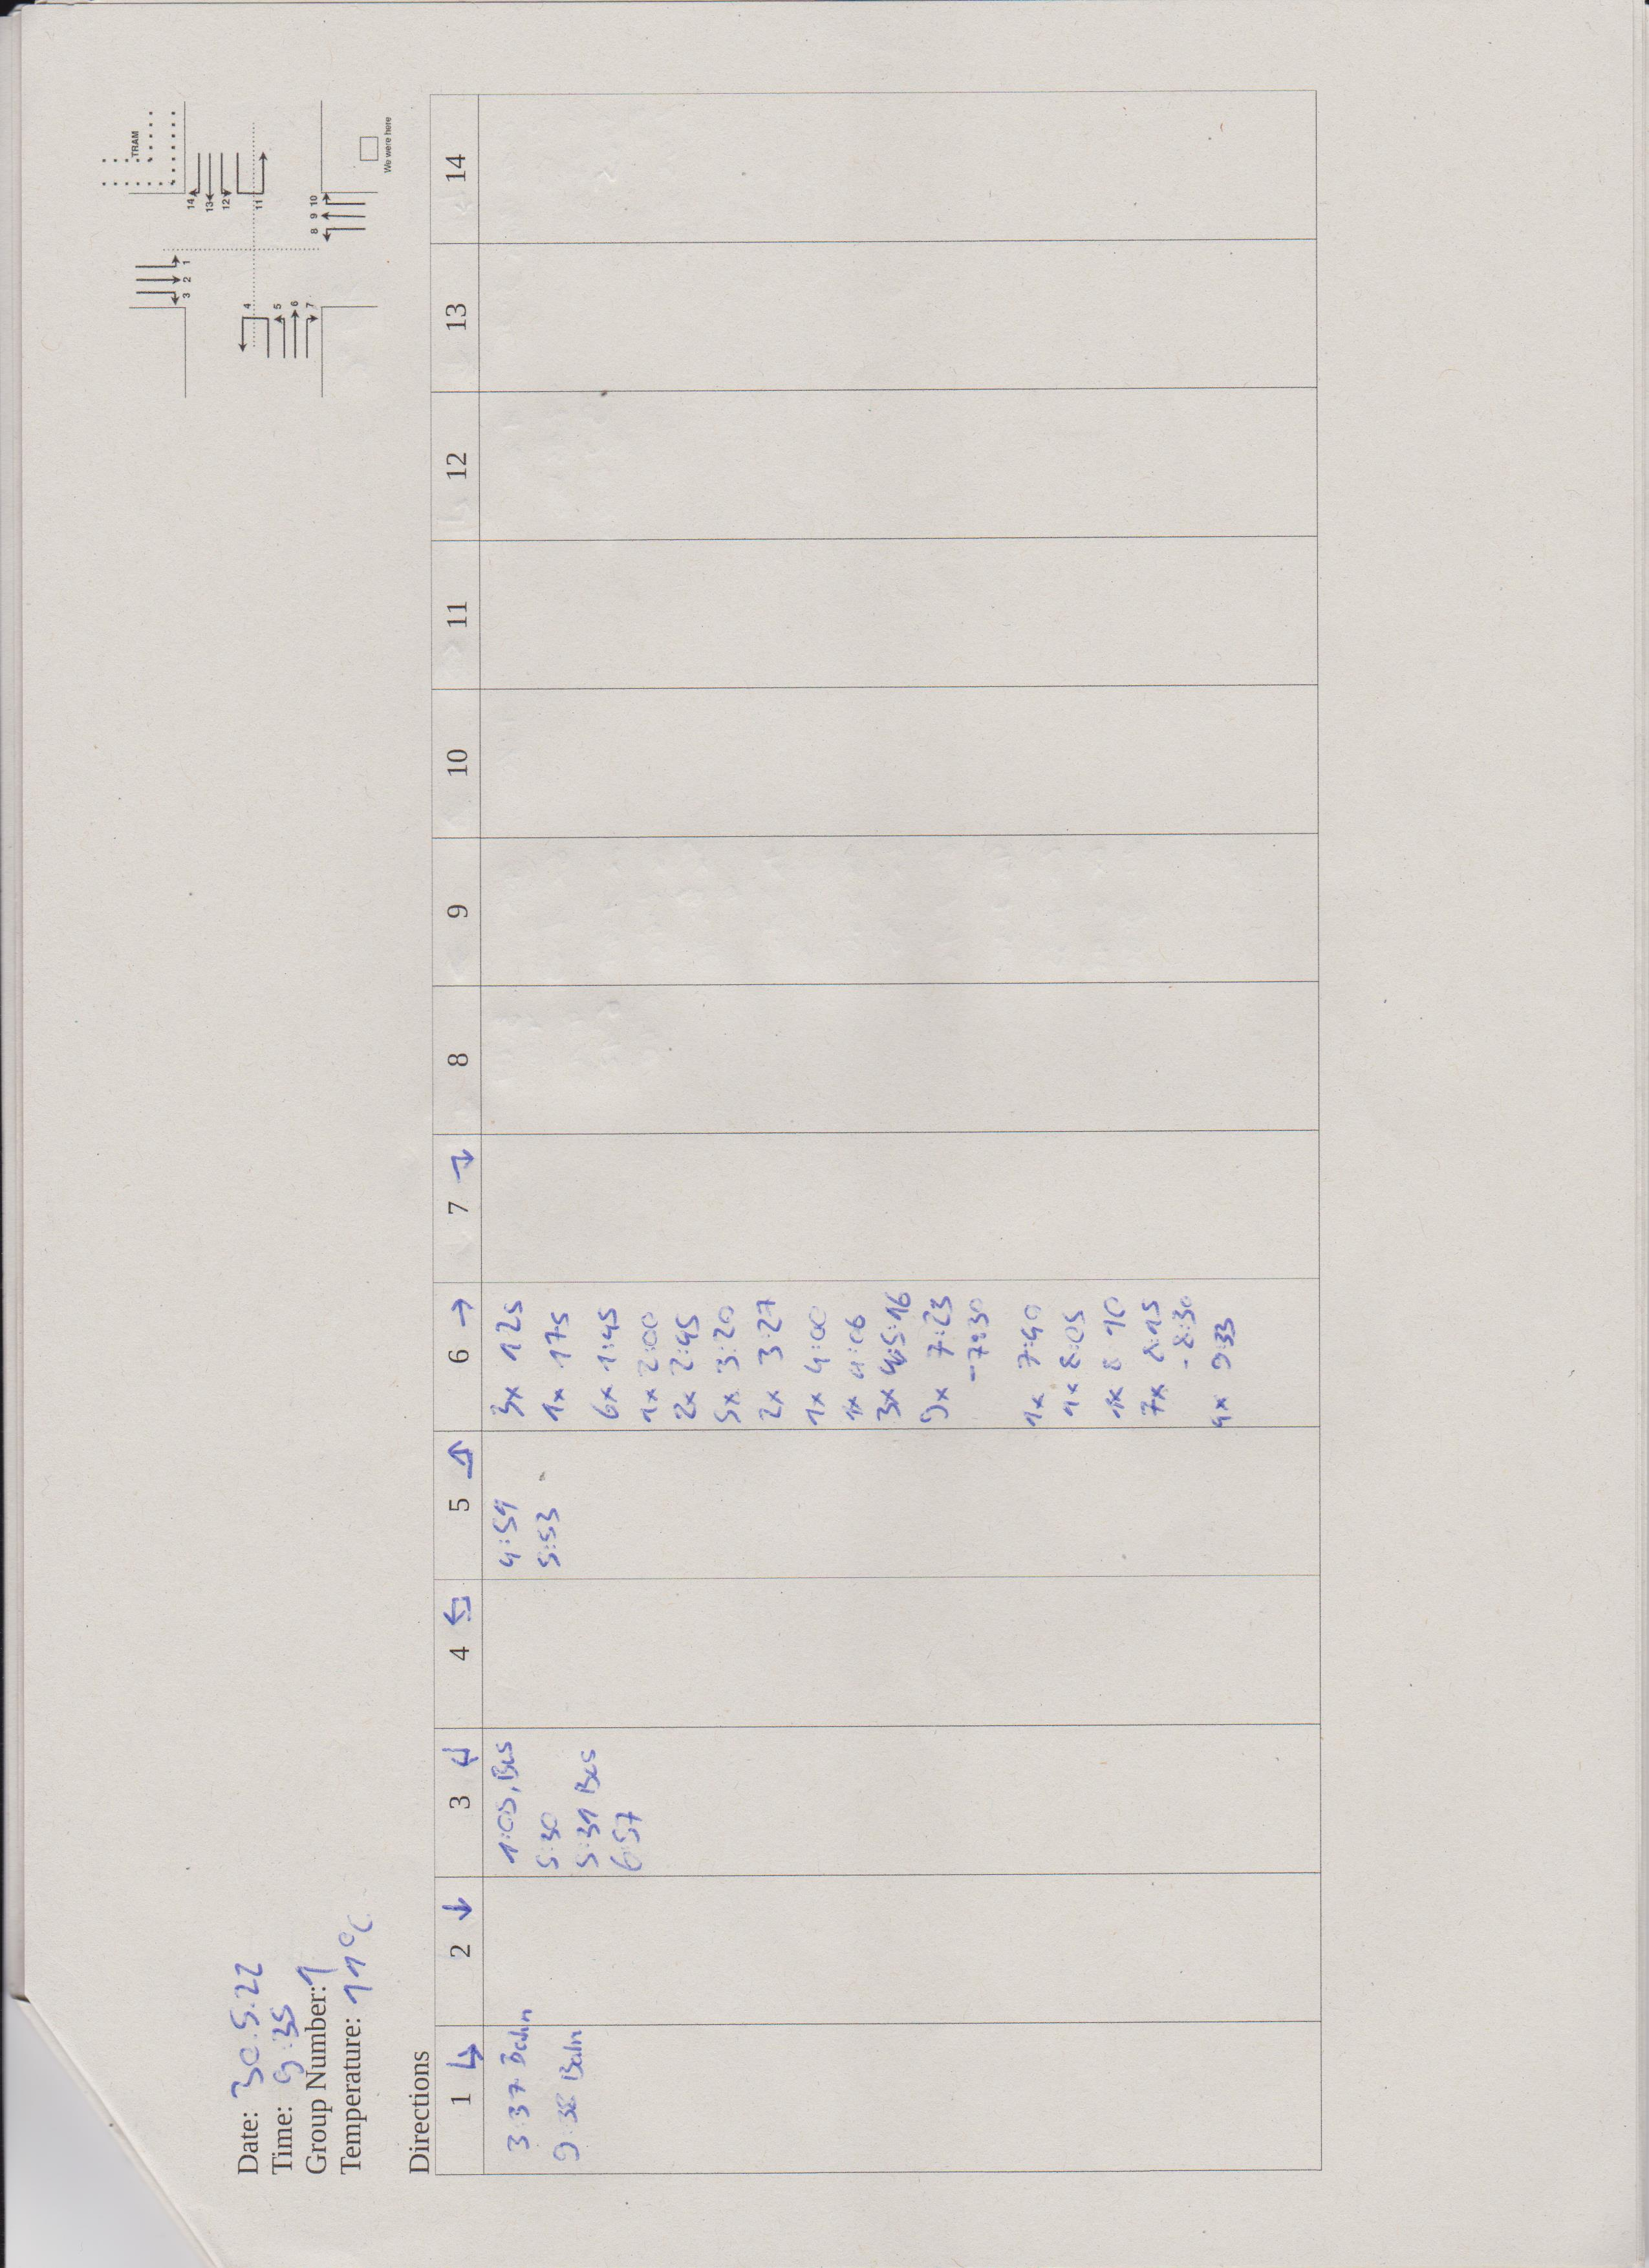
\includegraphics[width=\linewidth]{scans/Bild (7).jpg}
\end{figure*}

\begin{figure*}[htbp]
  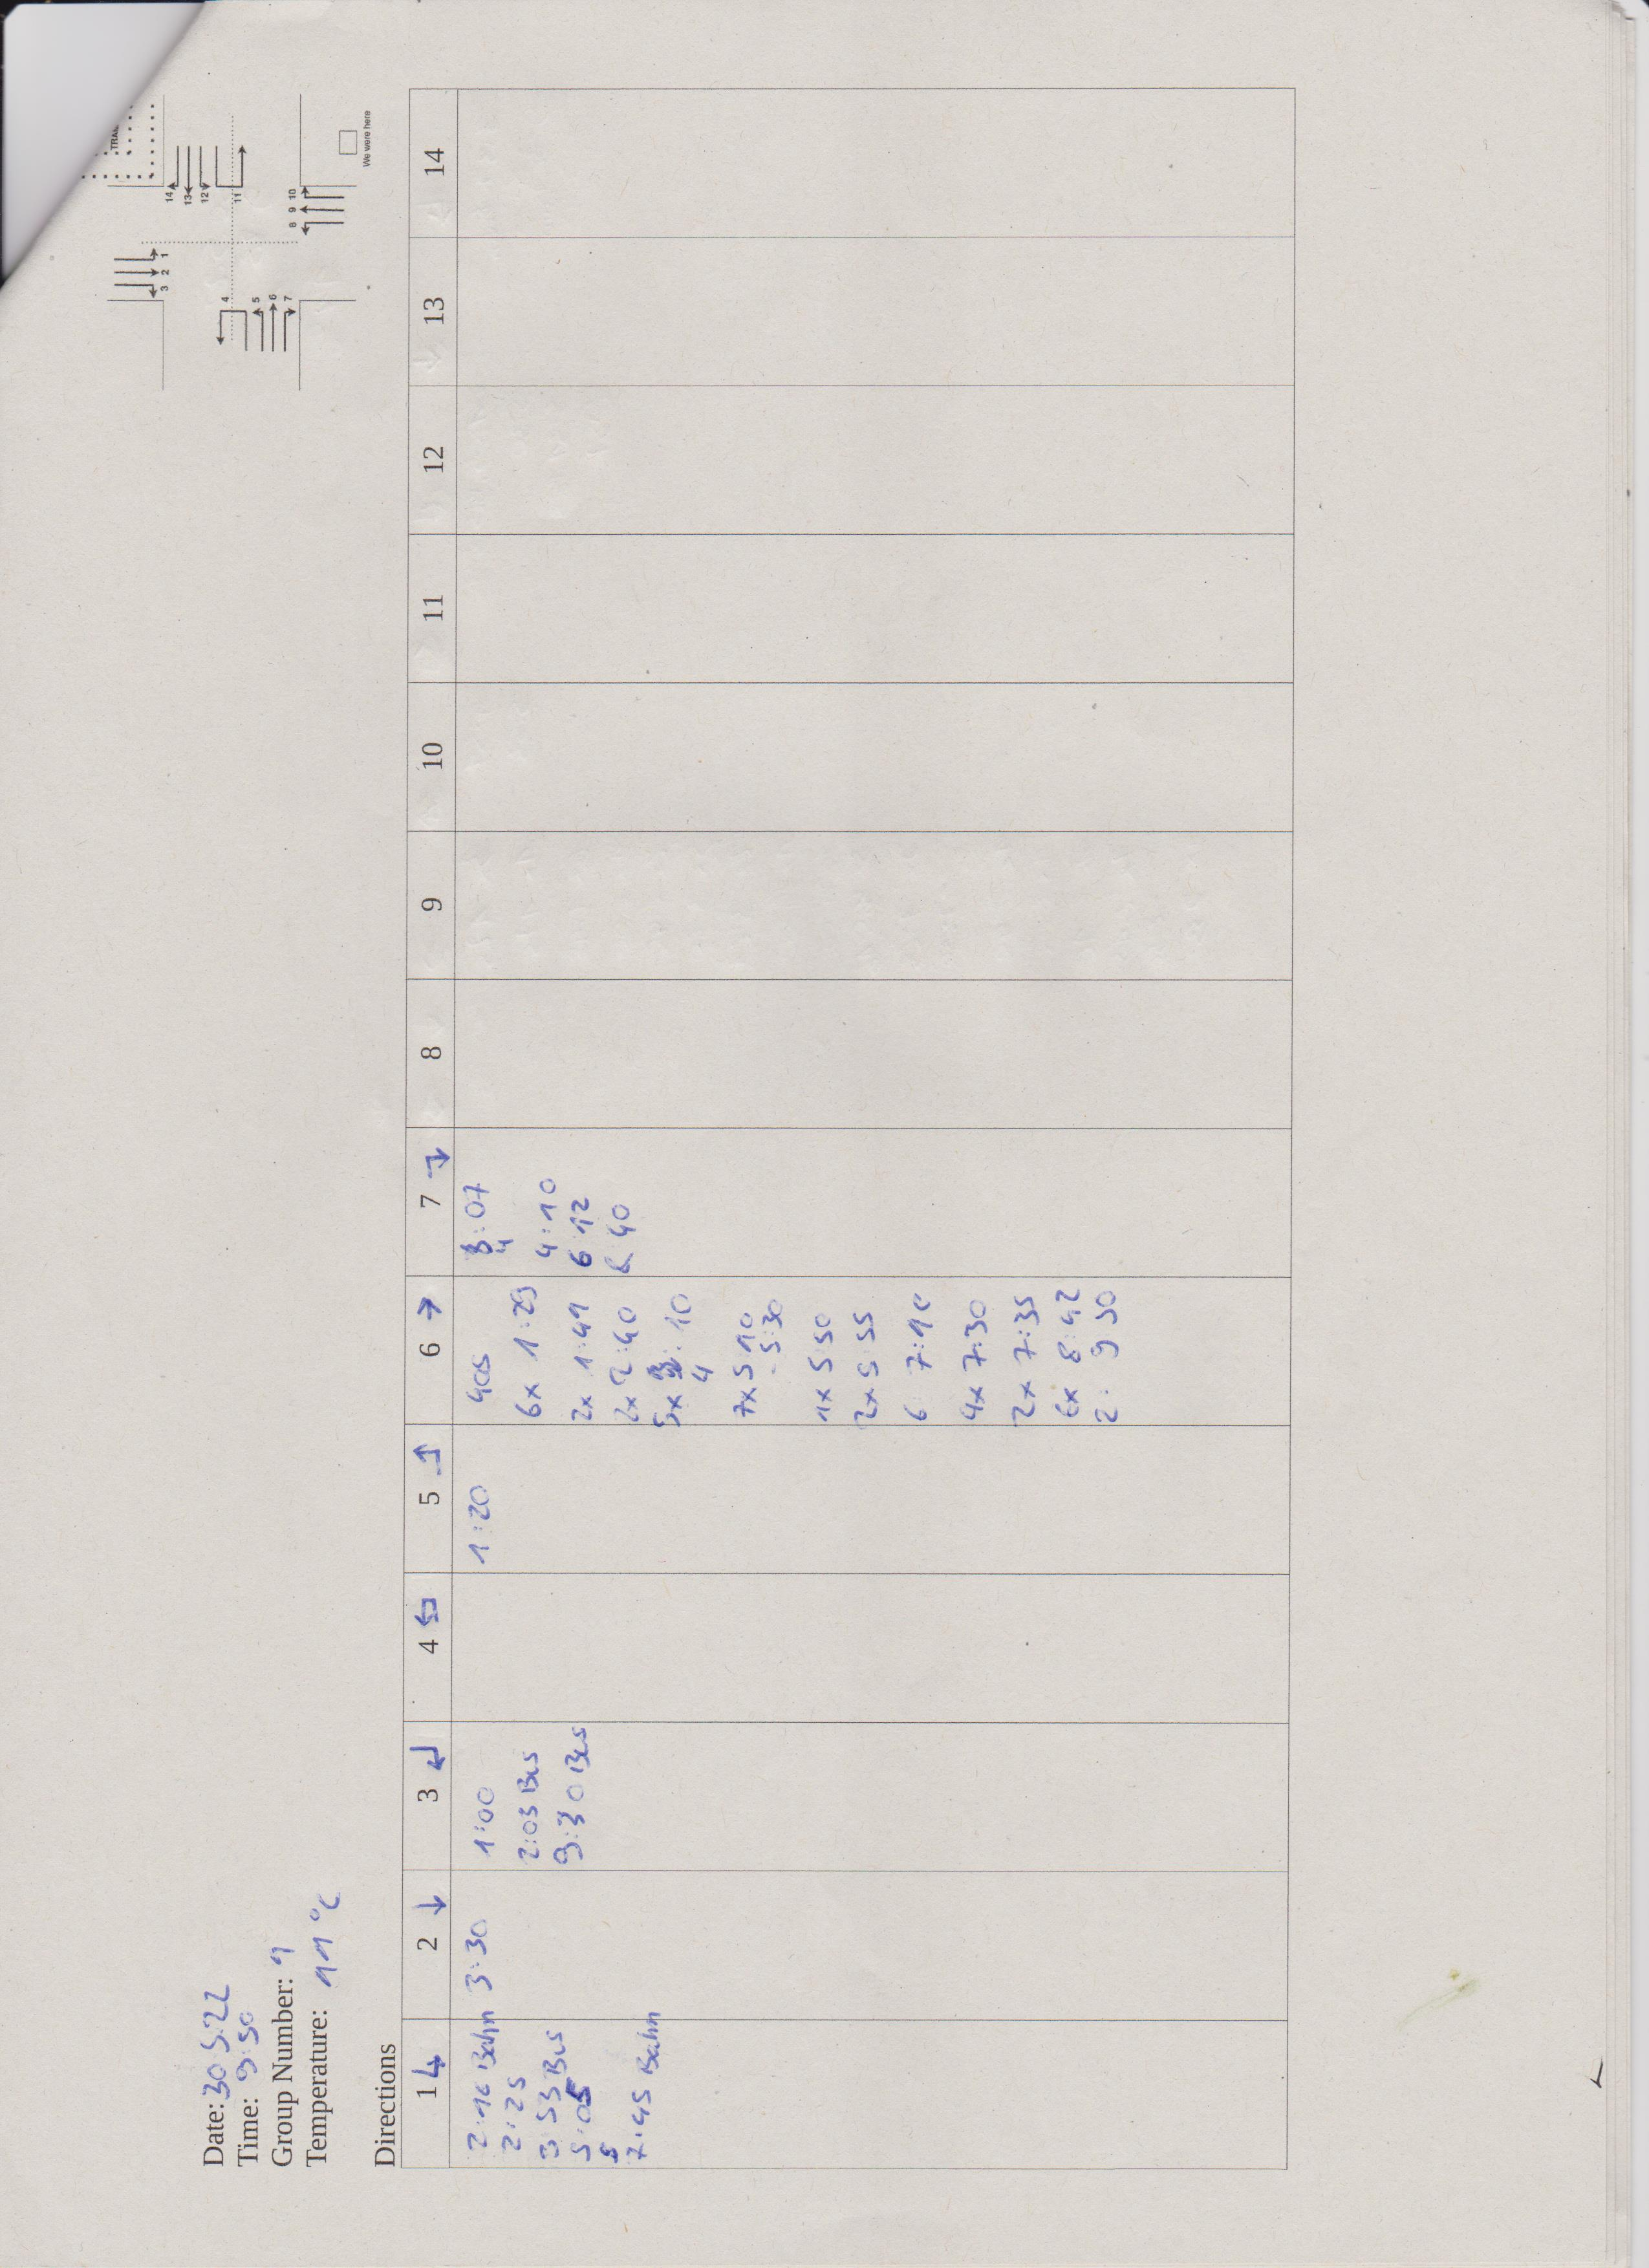
\includegraphics[width=\linewidth]{scans/Bild (8).jpg}
\end{figure*}

\begin{figure*}[htbp]
  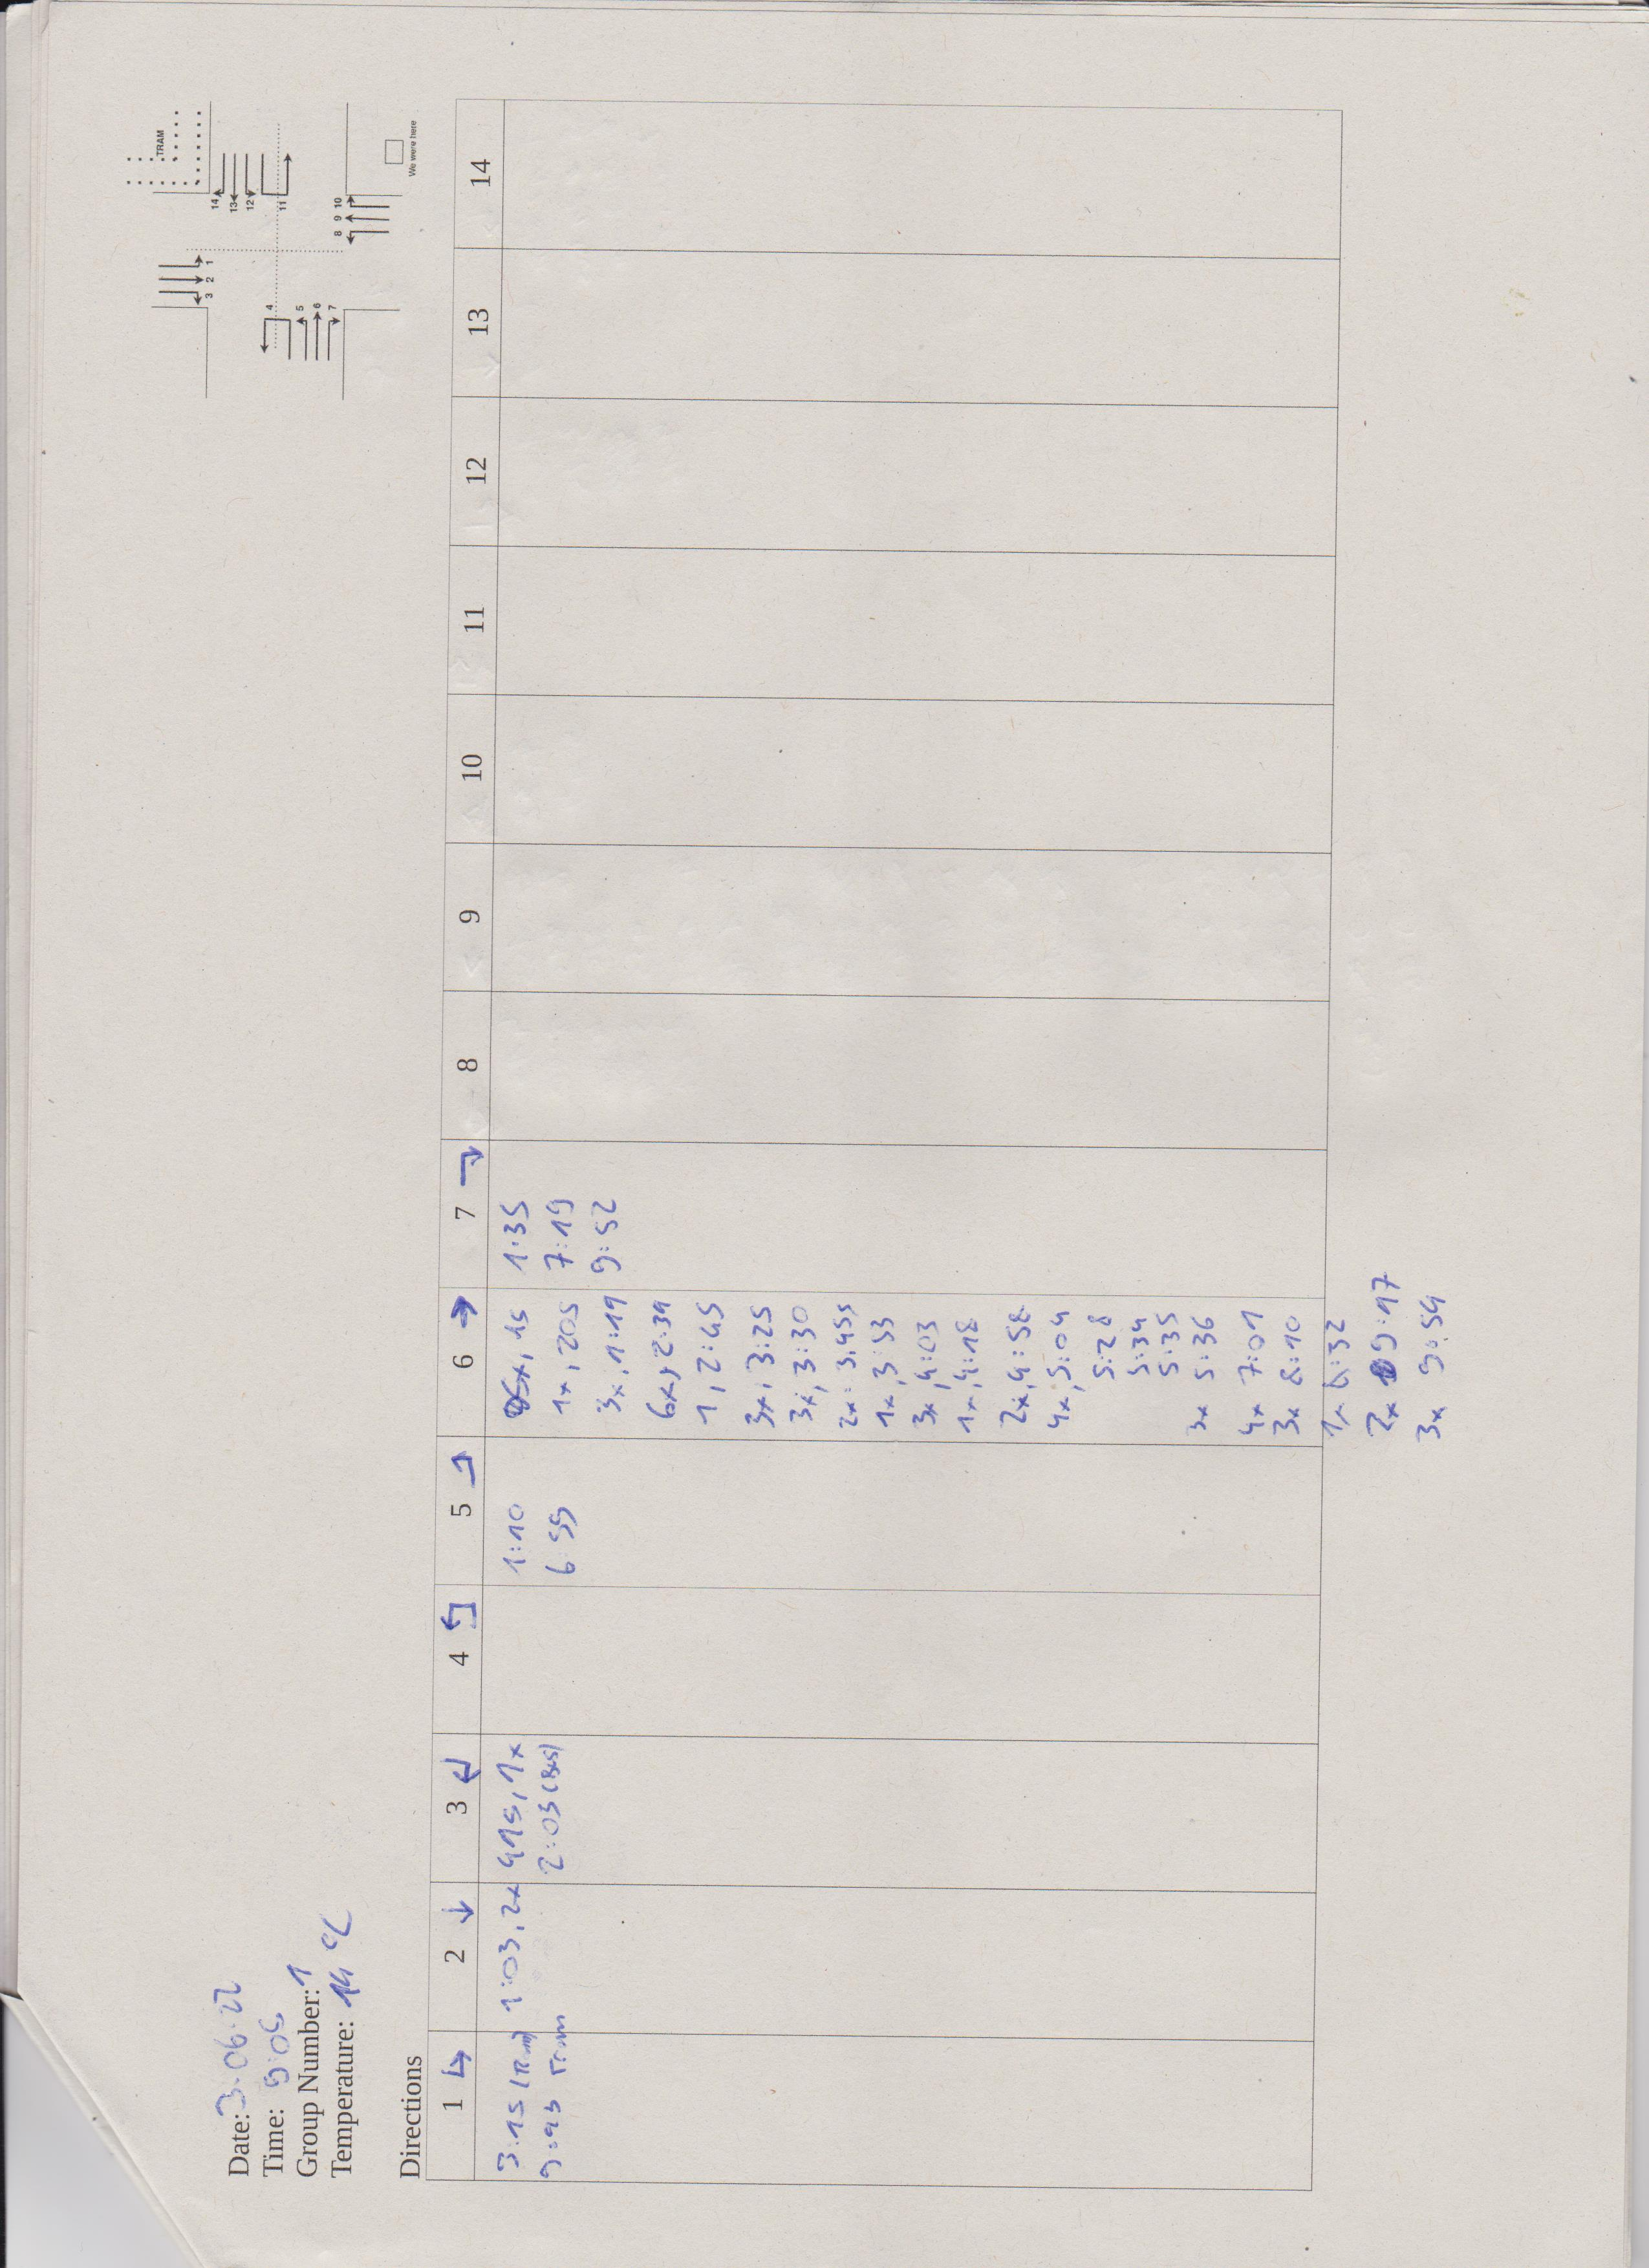
\includegraphics[width=\linewidth]{scans/Bild (9).jpg}
\end{figure*}

\begin{figure*}[htbp]
  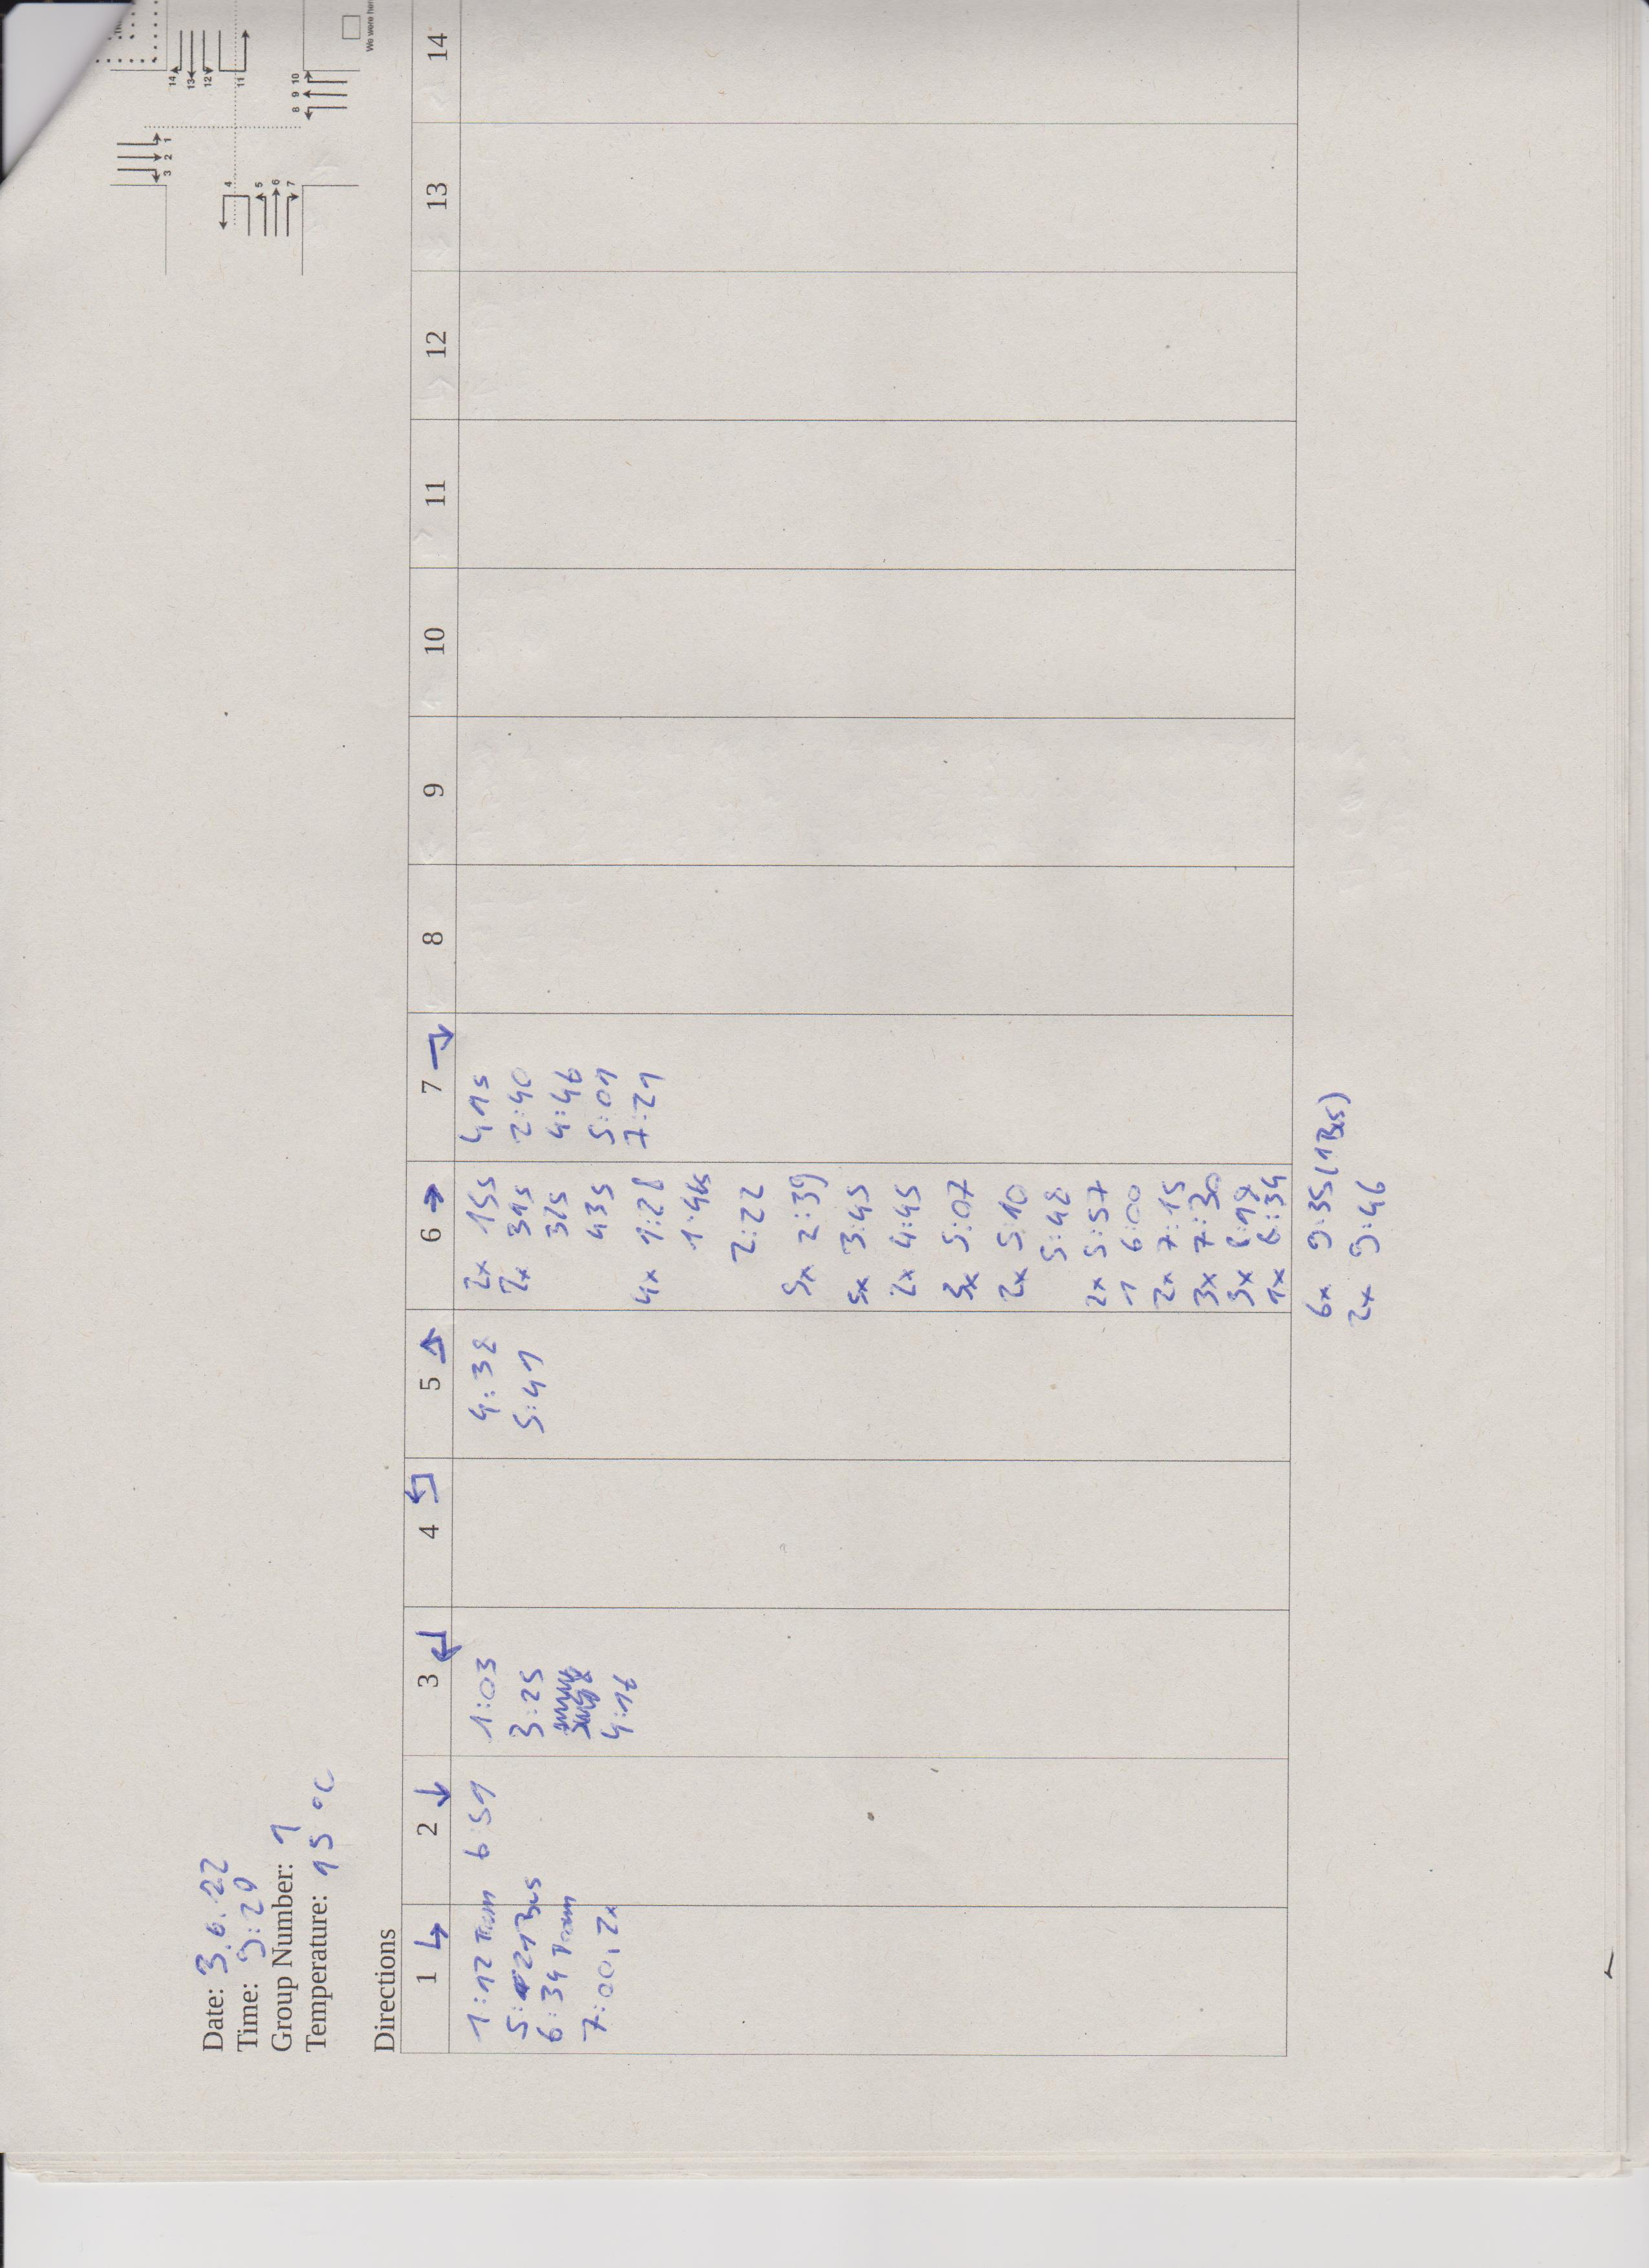
\includegraphics[width=\linewidth]{scans/Bild (10).jpg}
\end{figure*}

\begin{figure*}[htbp]
  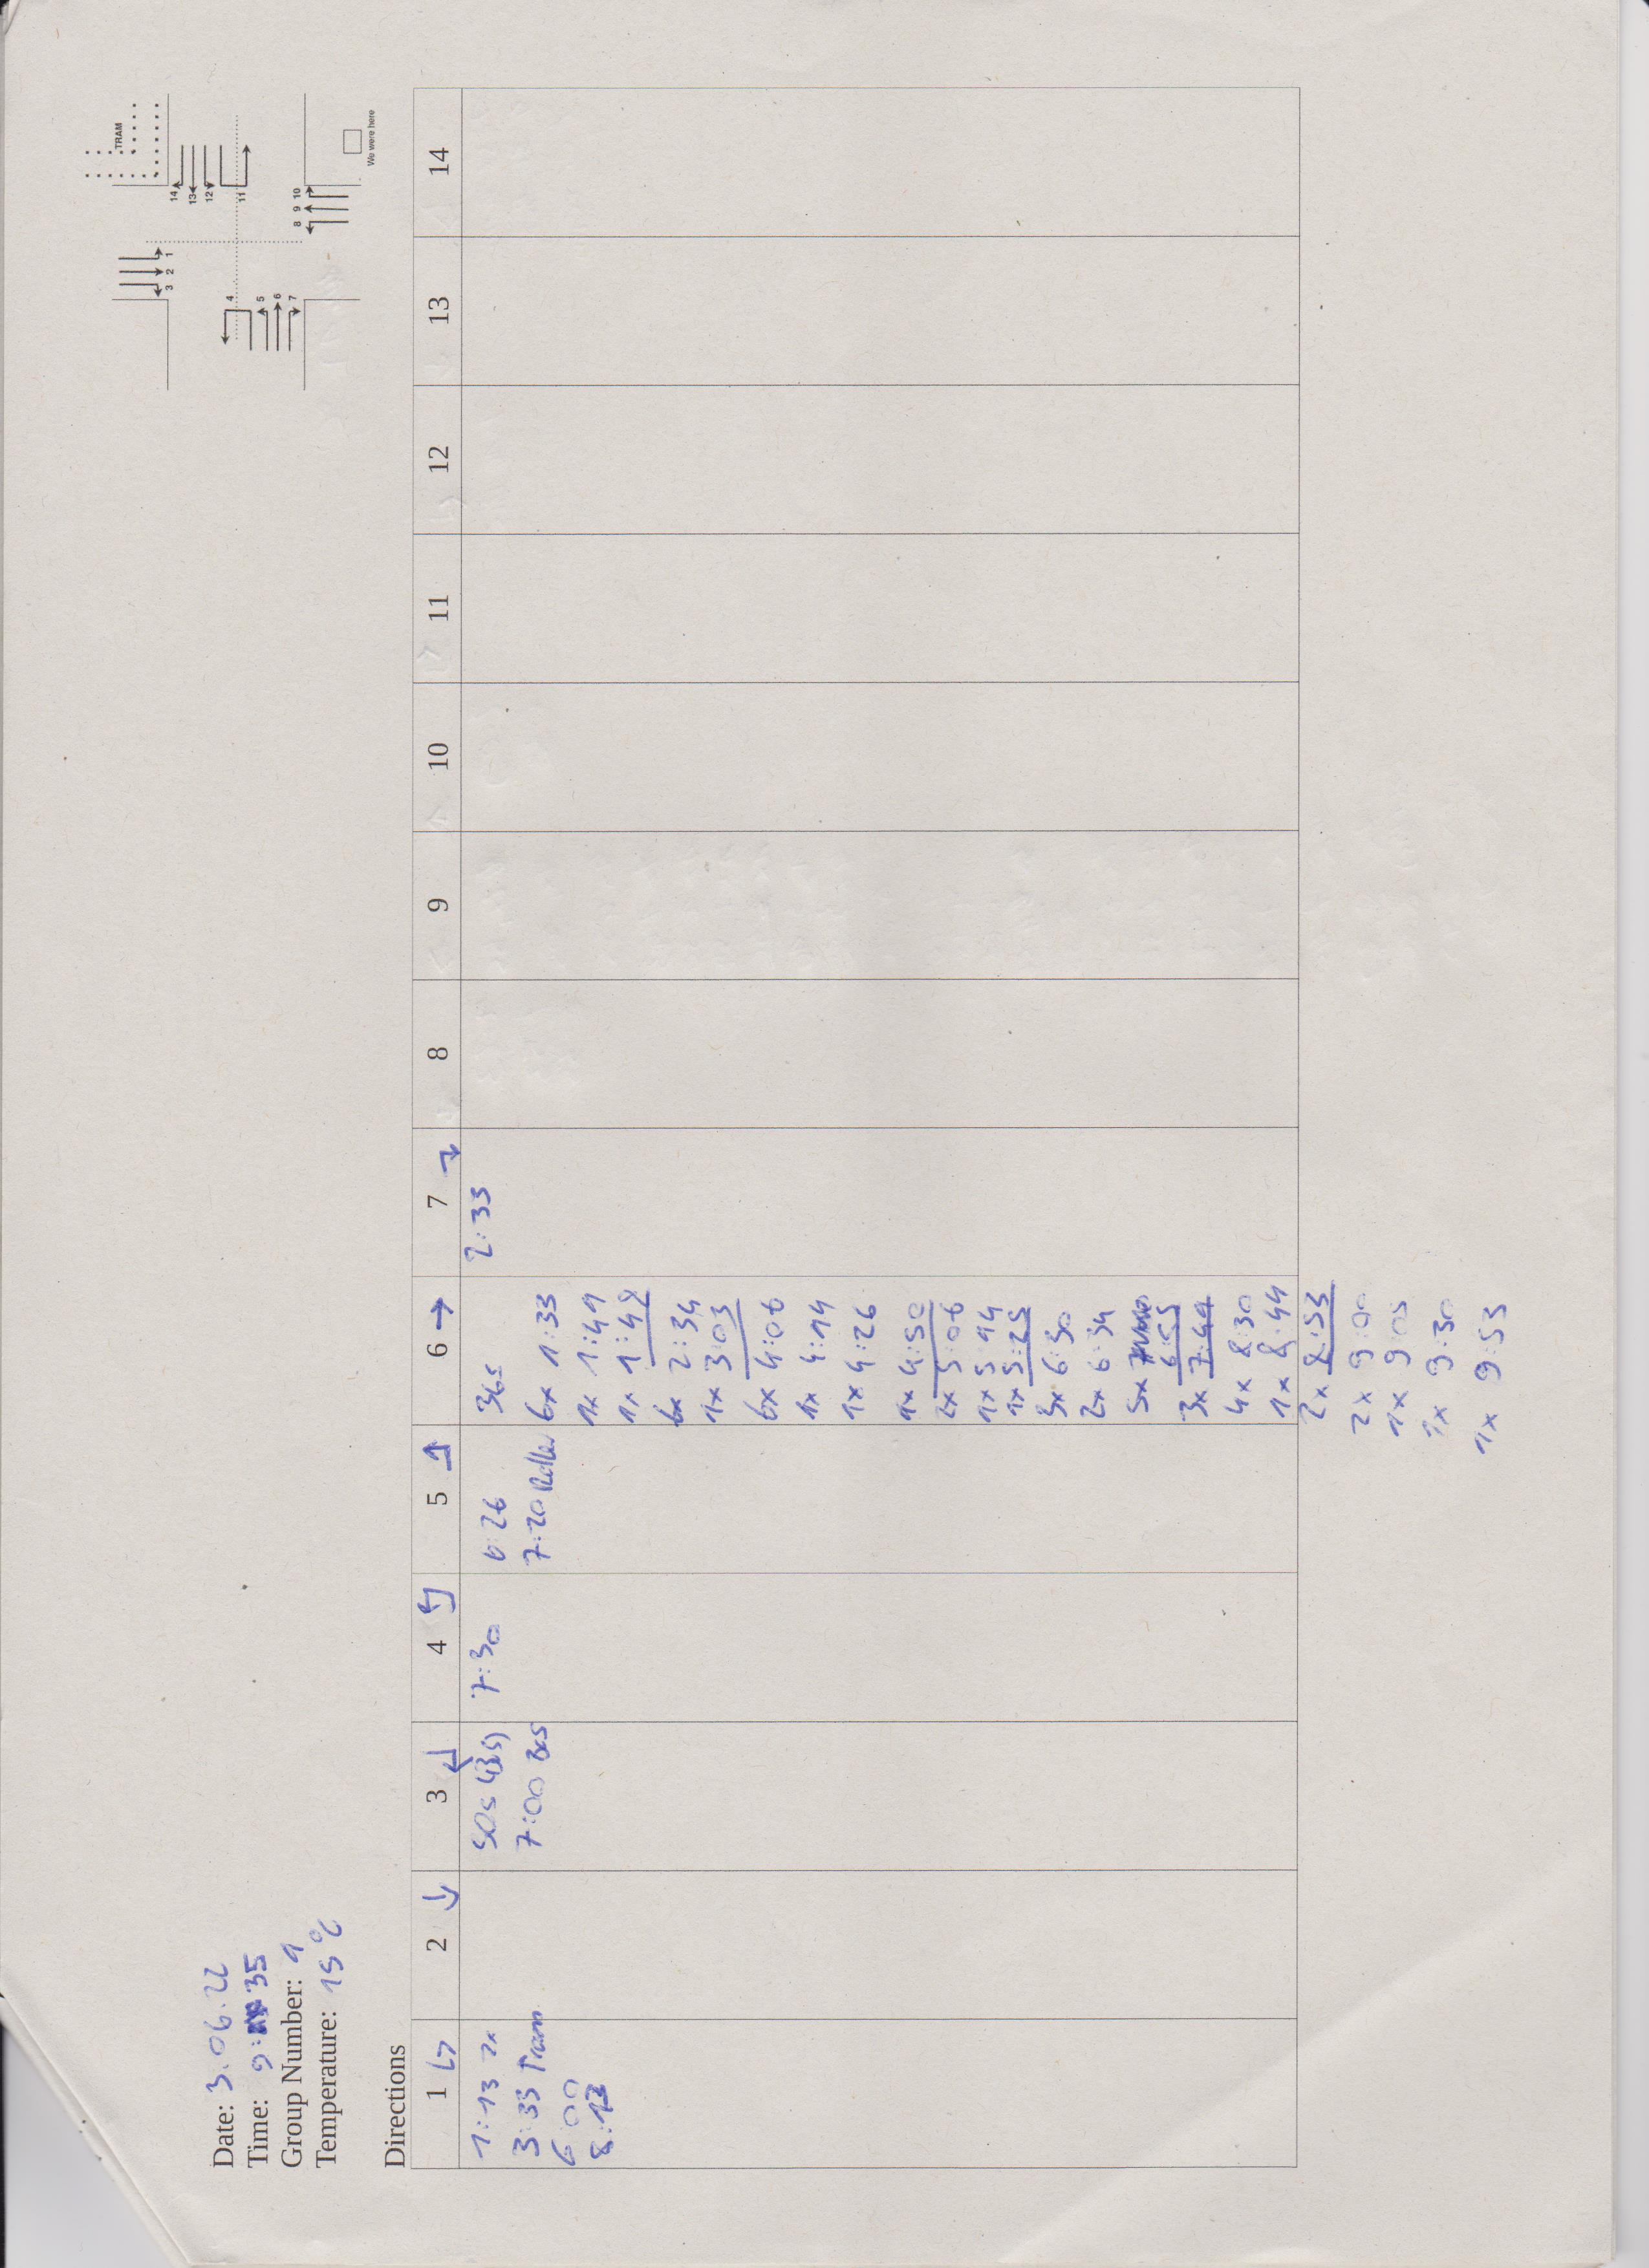
\includegraphics[width=\linewidth]{scans/Bild (11).jpg}
\end{figure*}

\begin{figure*}[htbp]
  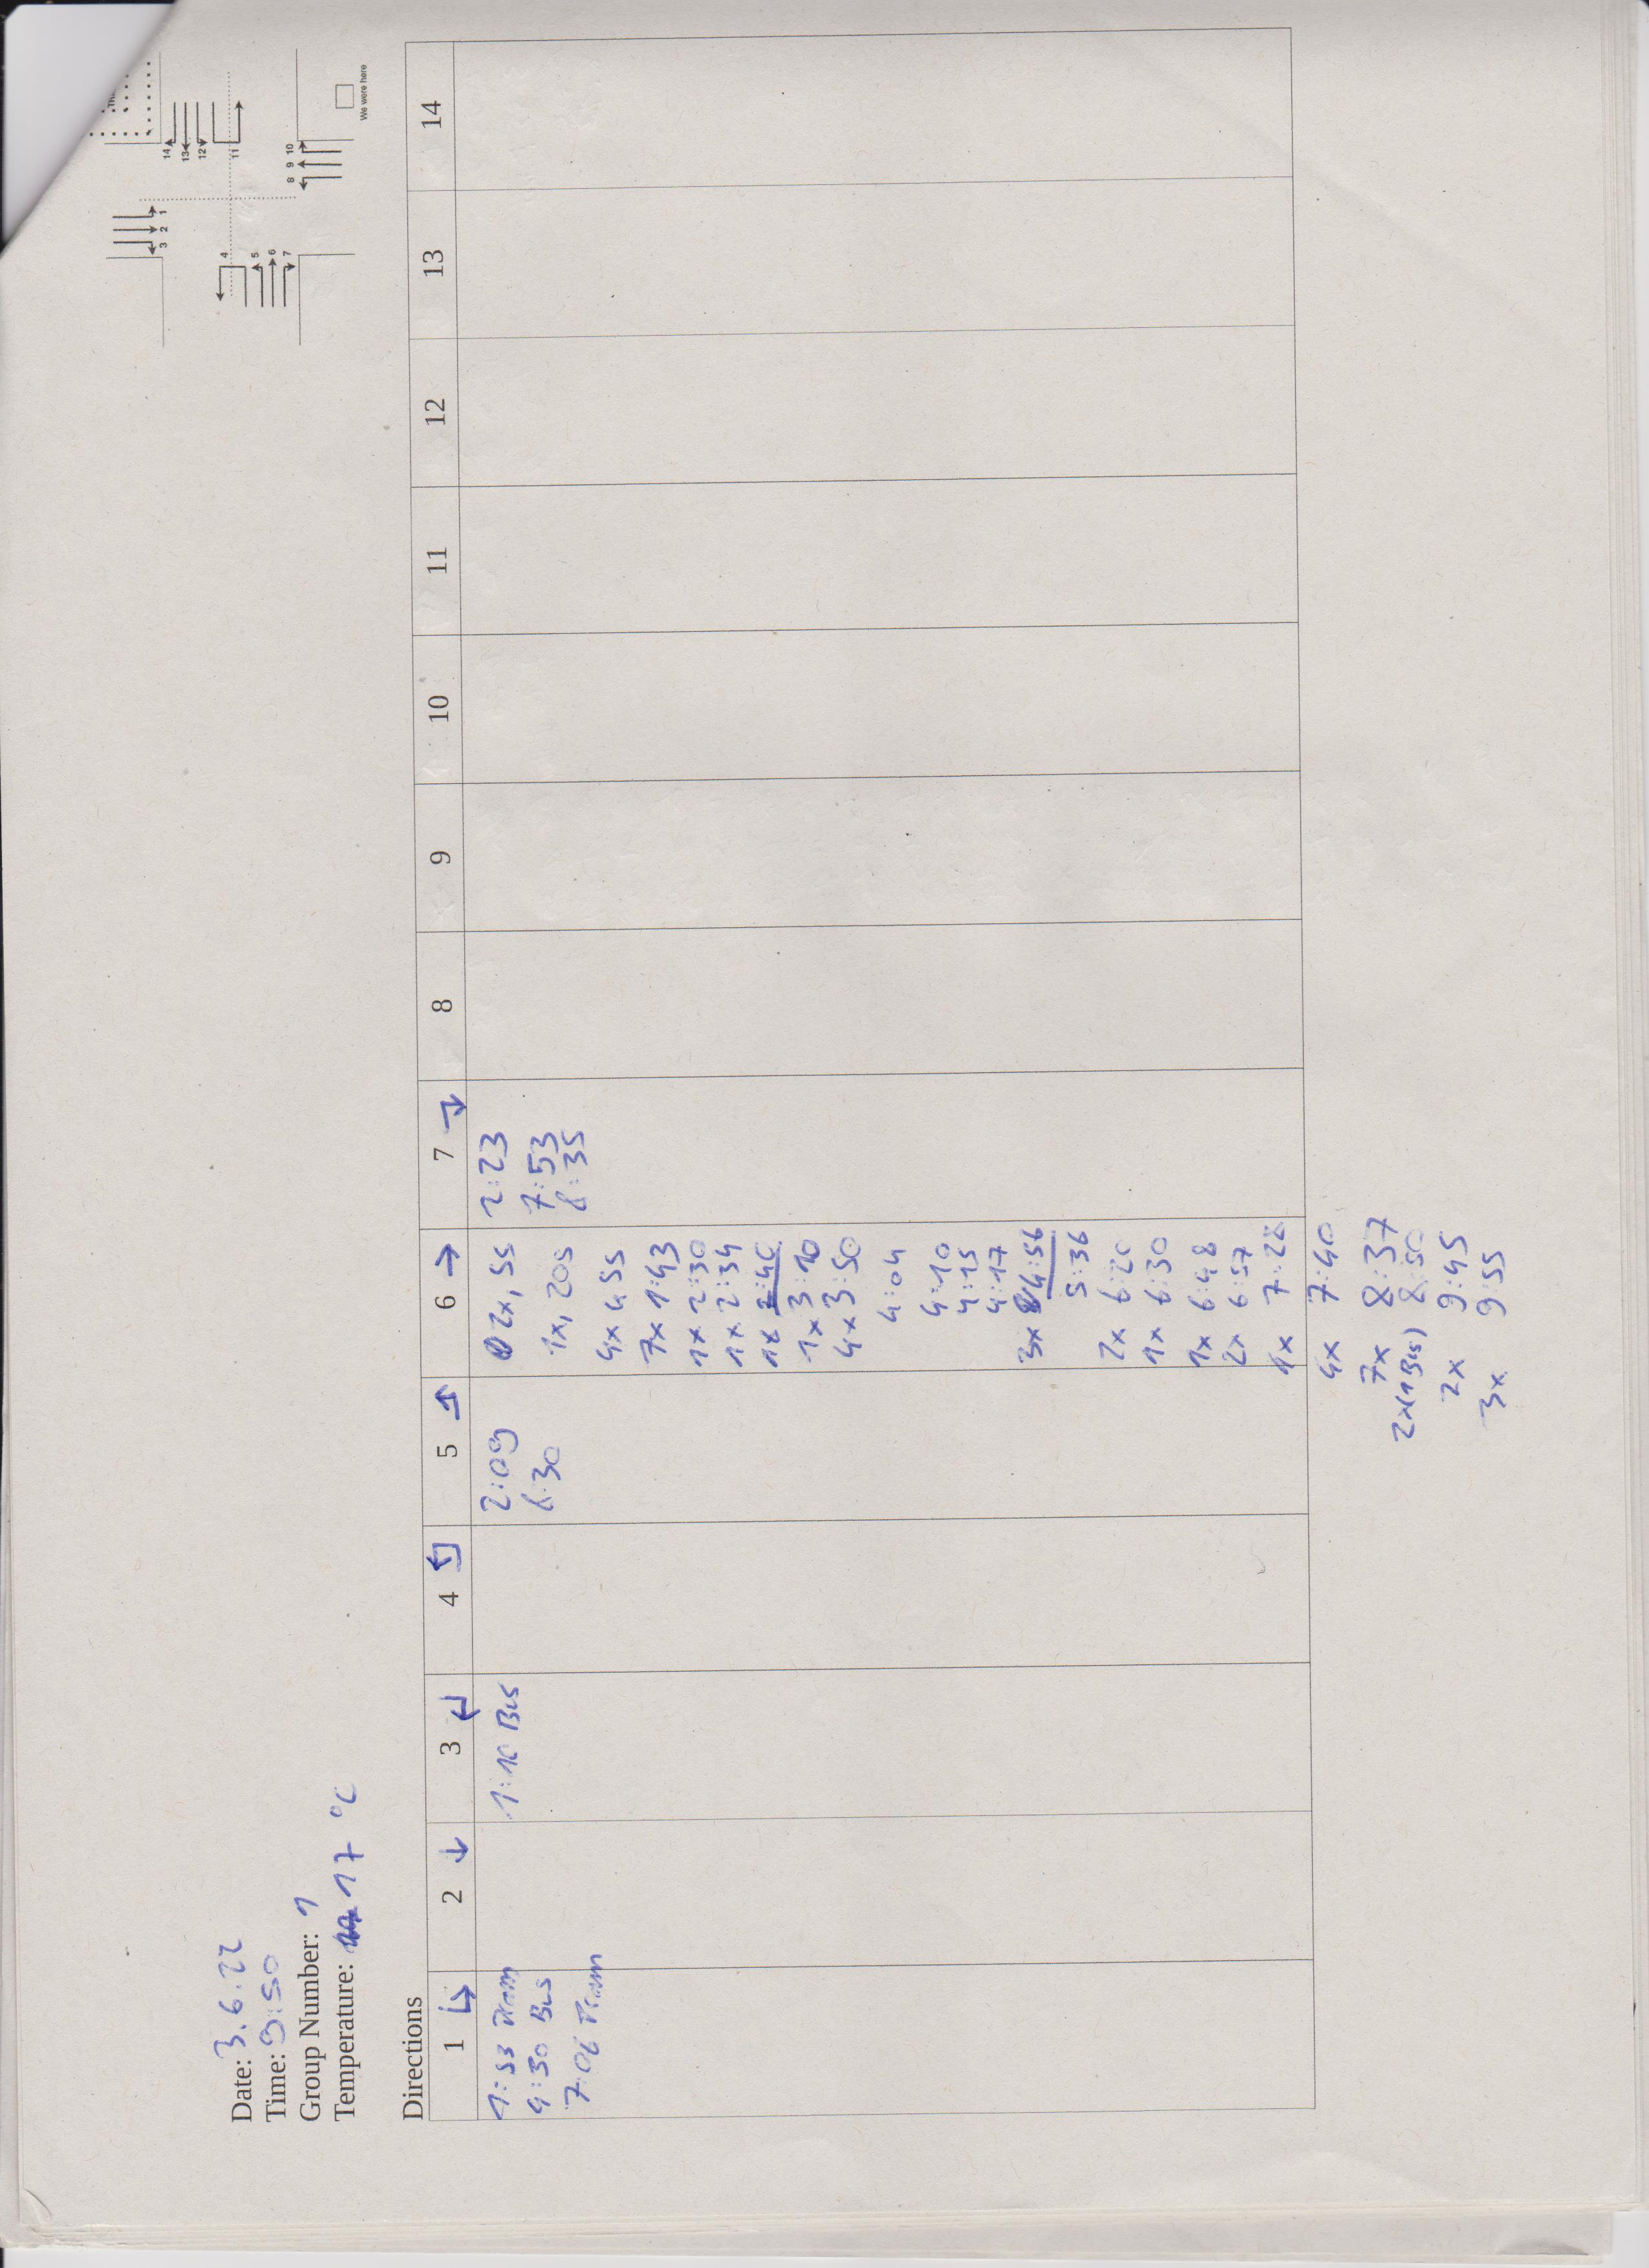
\includegraphics[width=\linewidth]{scans/Bild (12).jpg}
\end{figure*}

\begin{figure*}[htbp]
  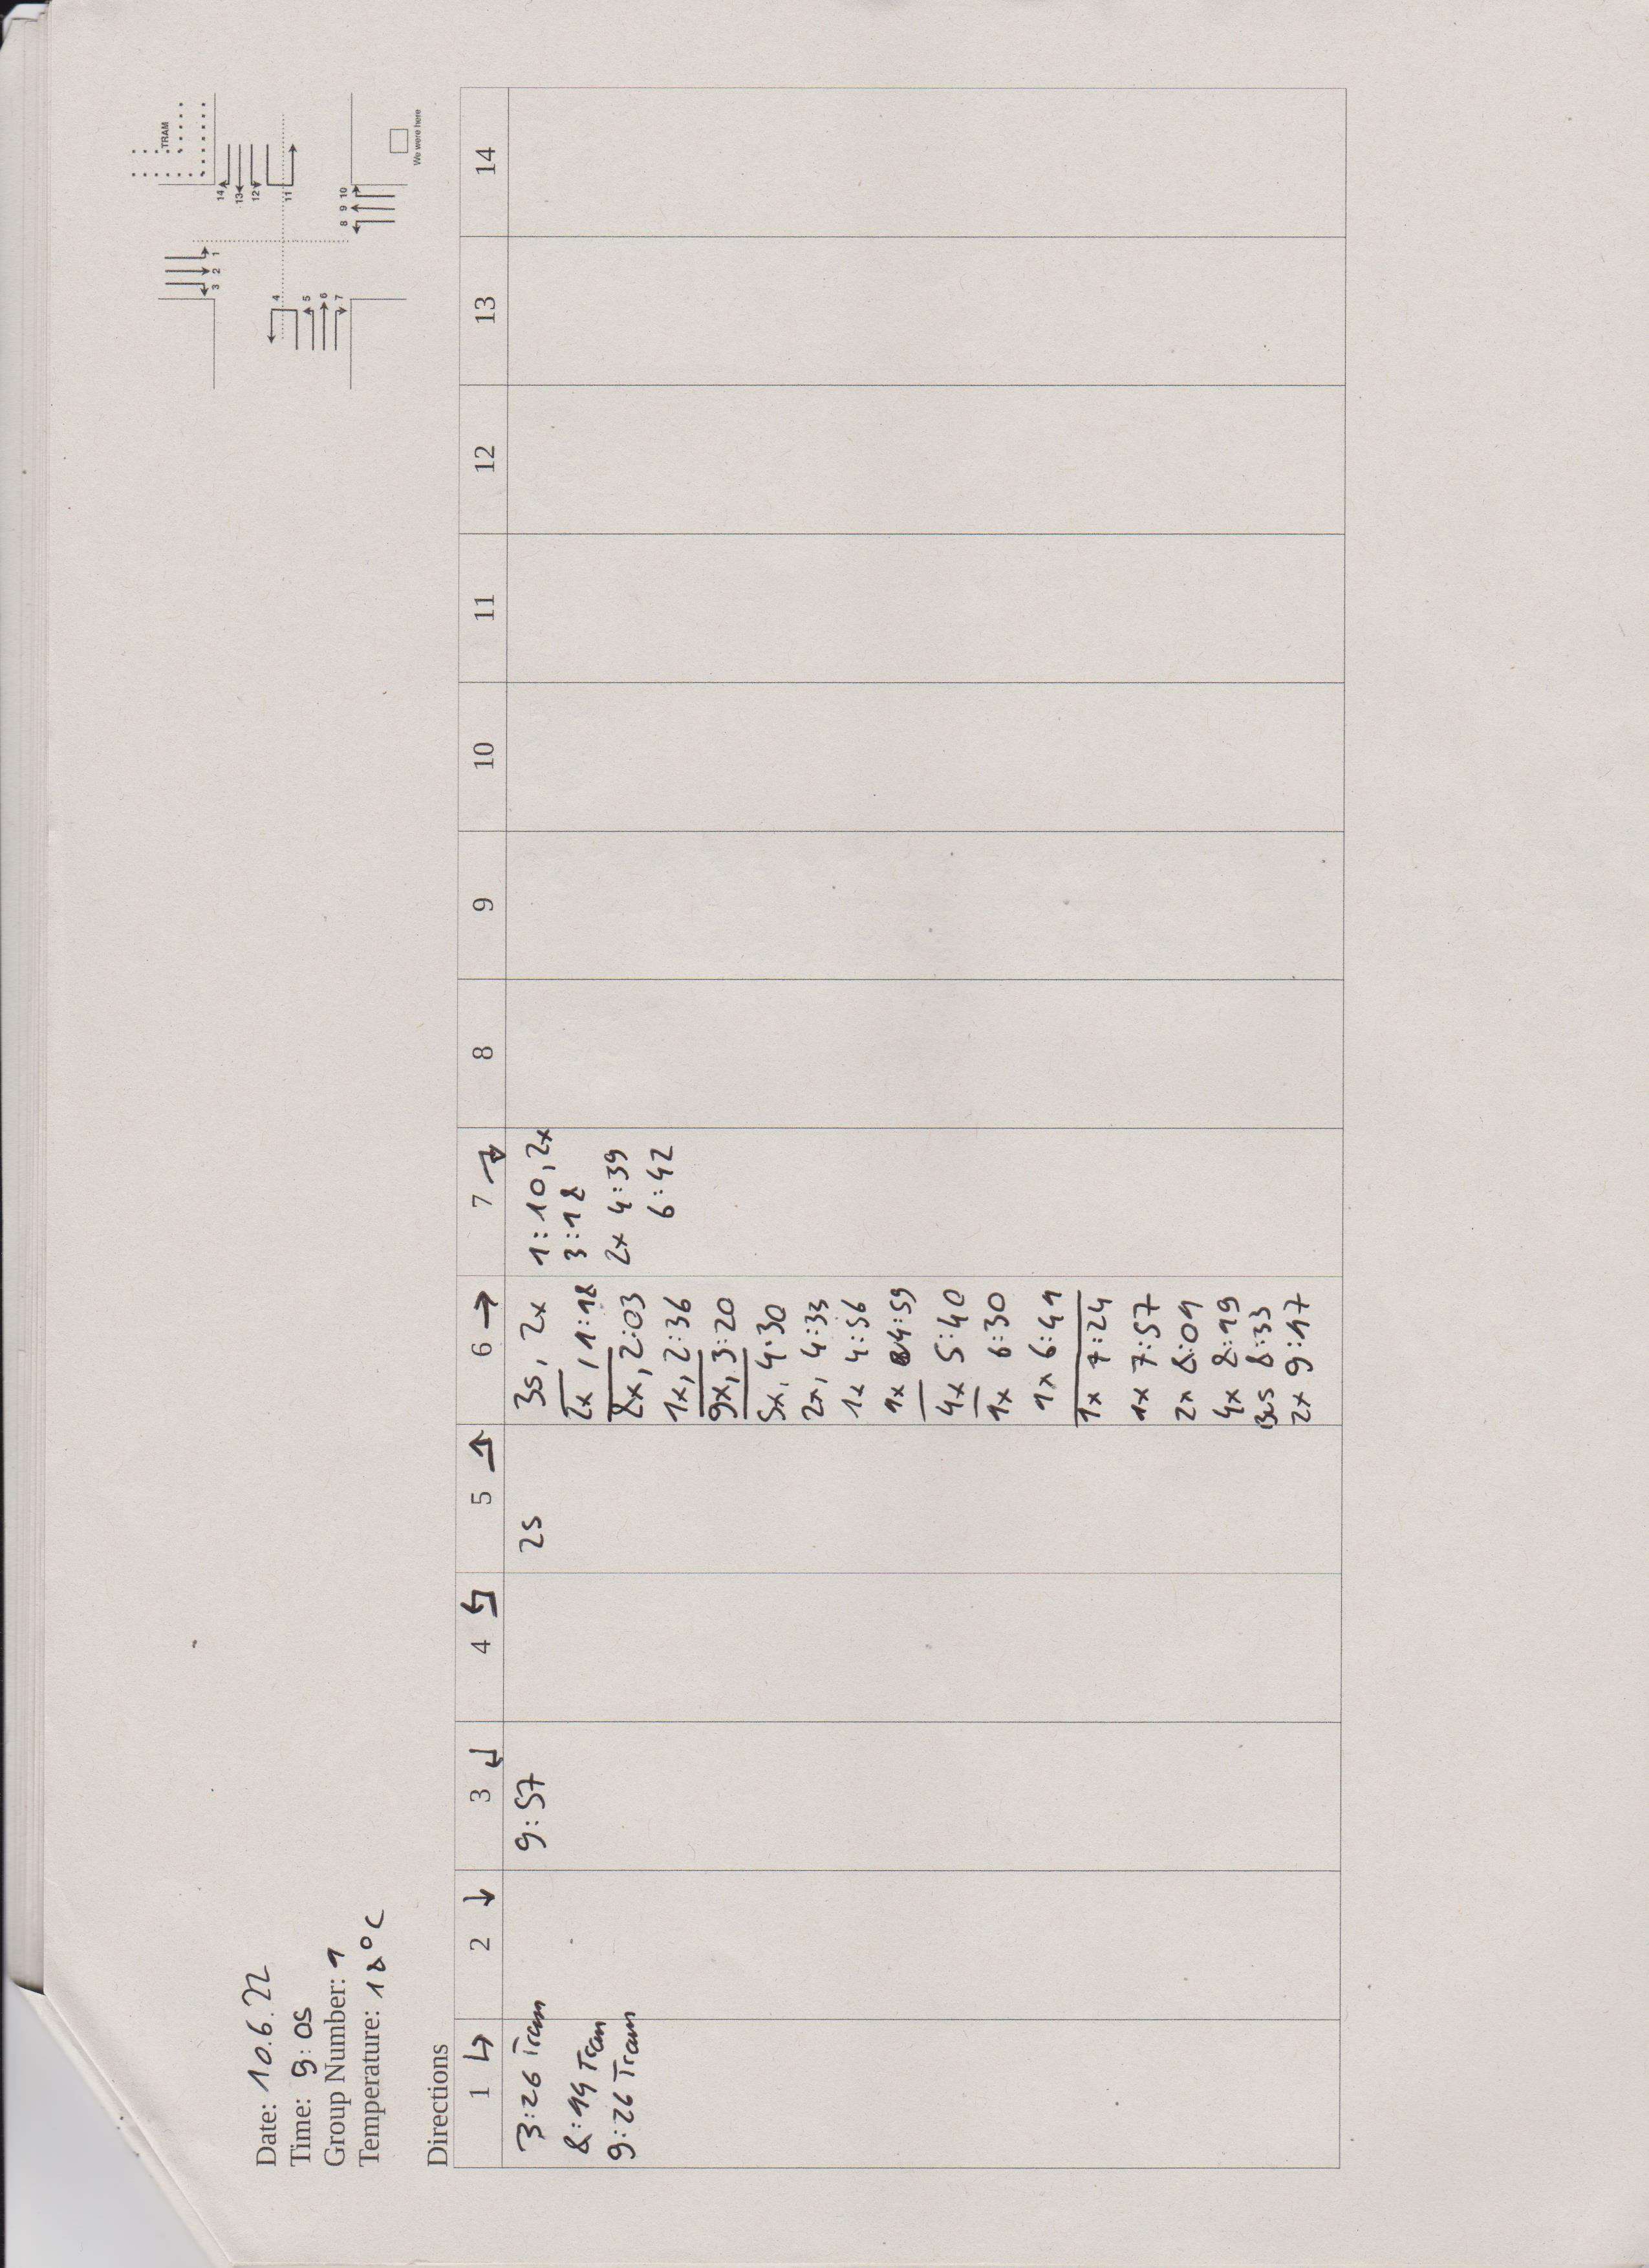
\includegraphics[width=\linewidth]{scans/Bild (13).jpg}
\end{figure*}

\begin{figure*}[htbp]
  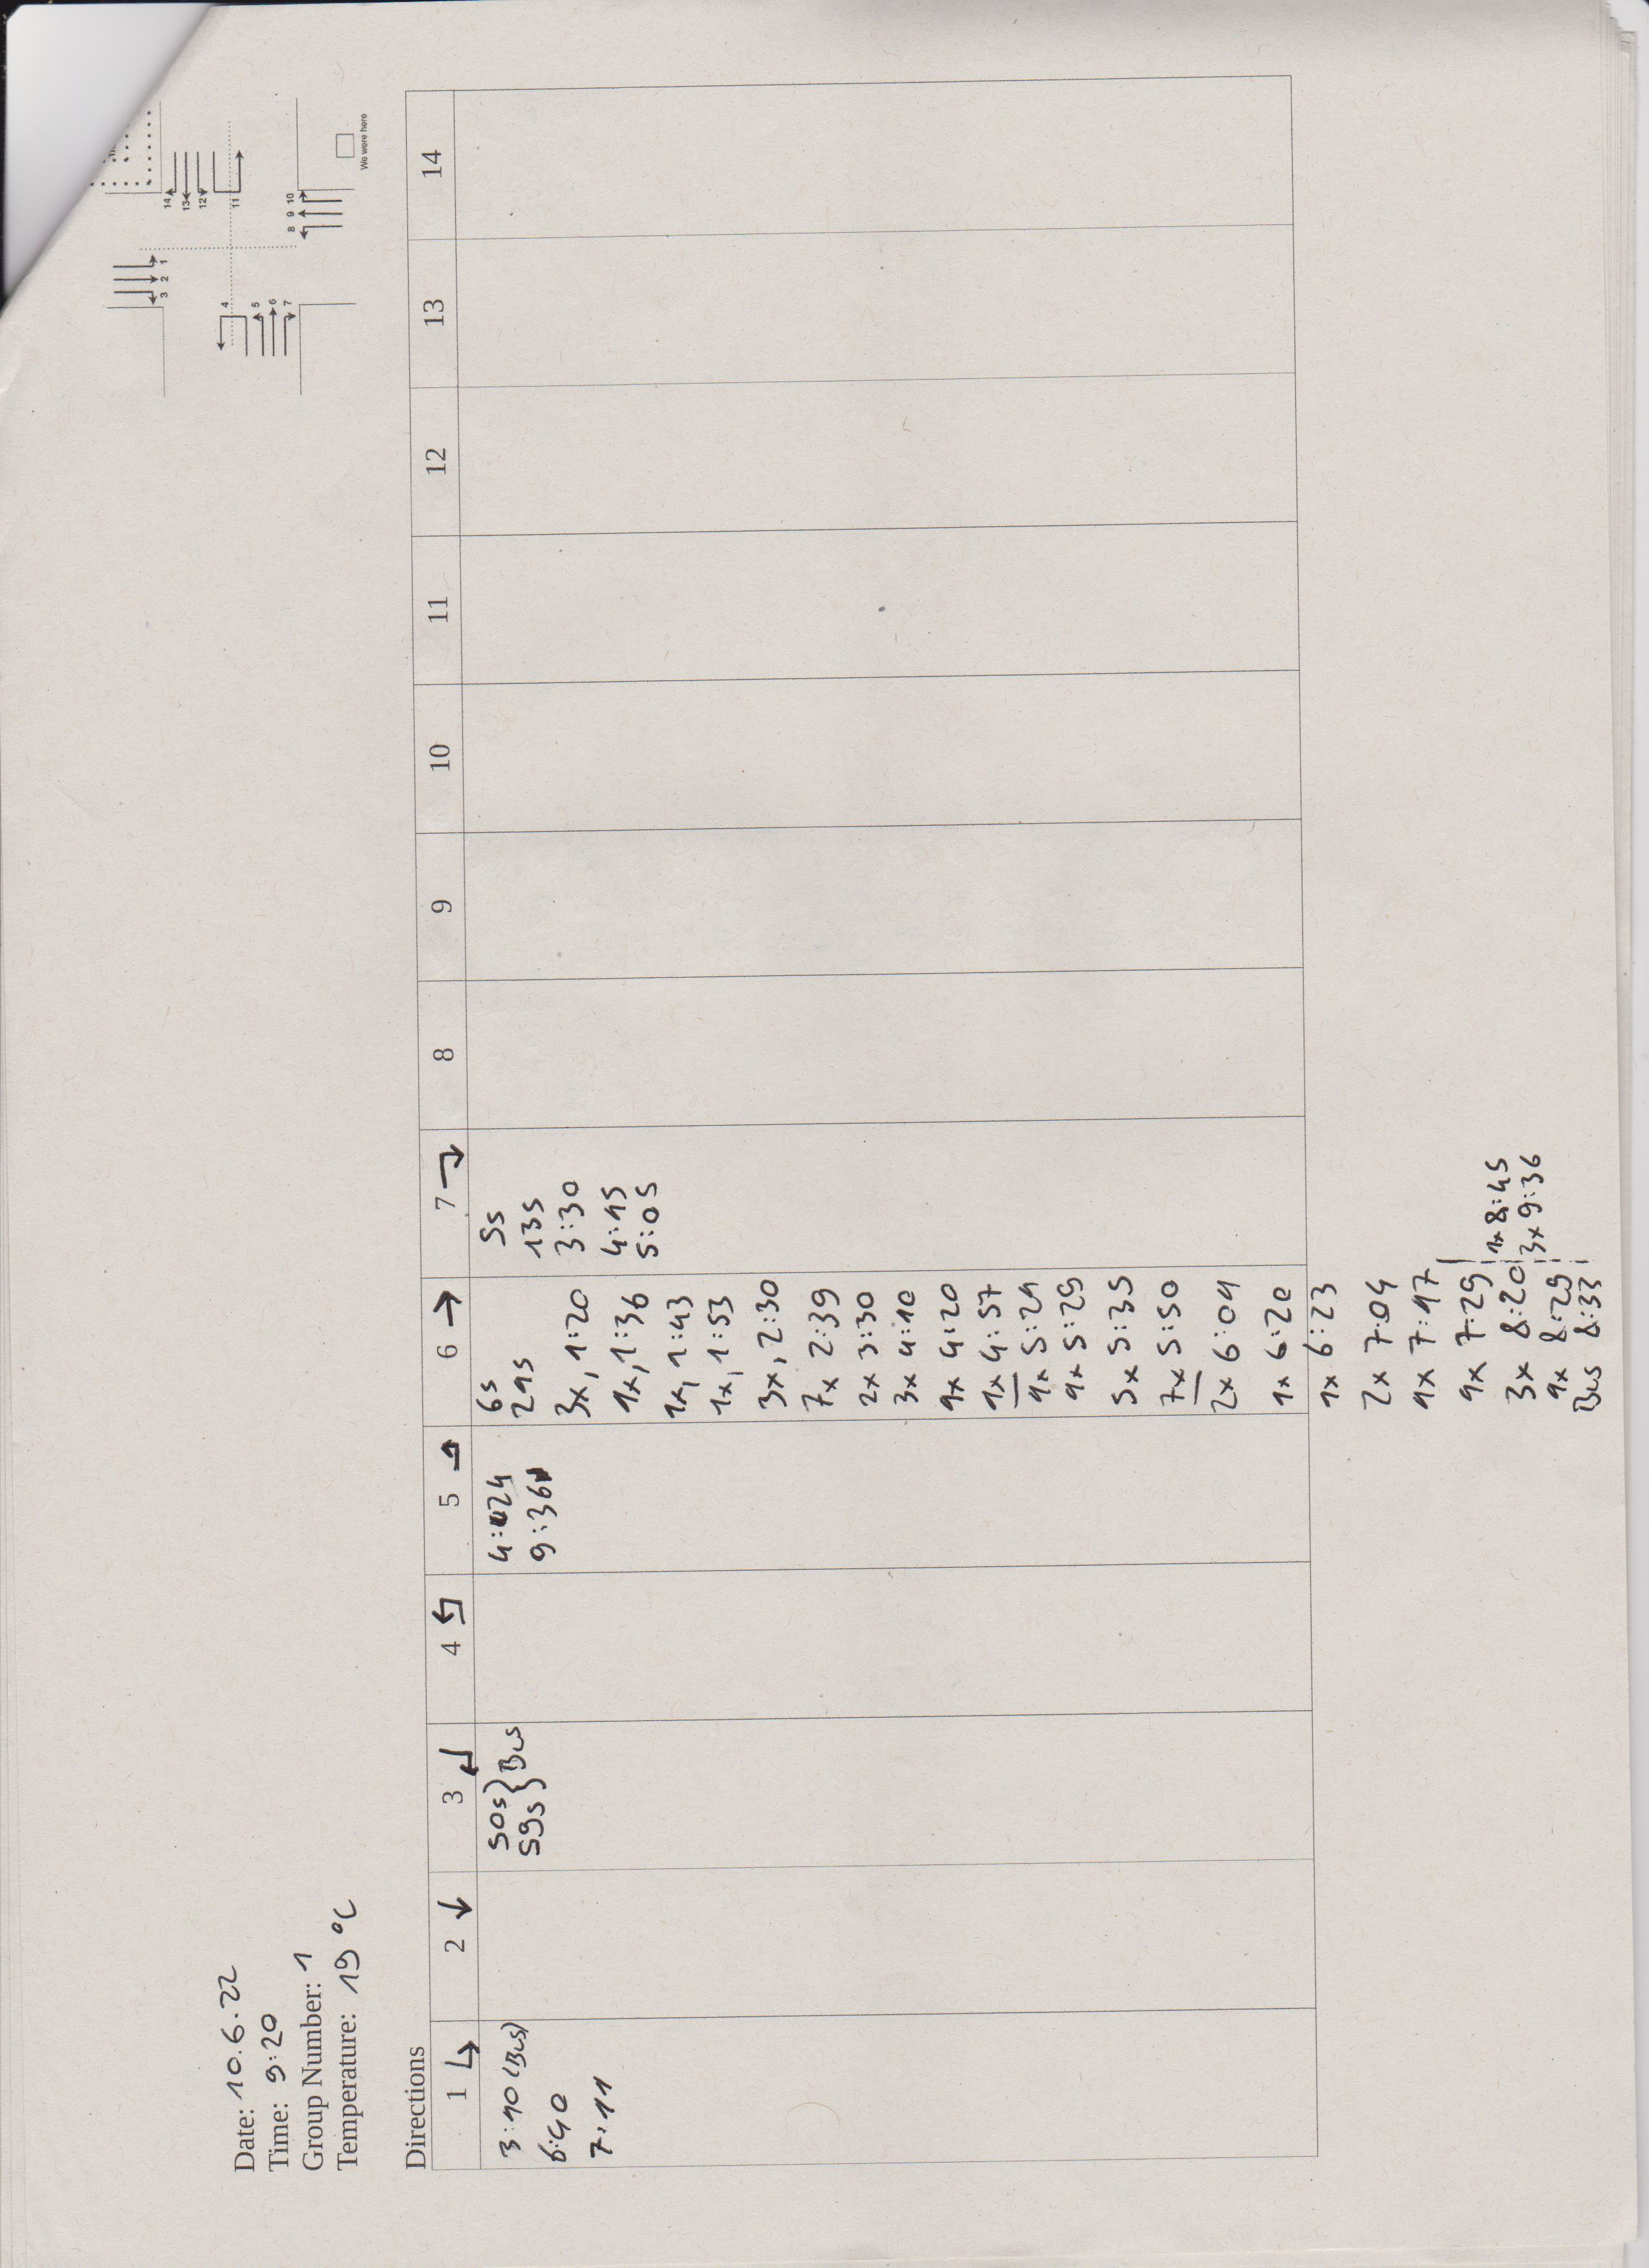
\includegraphics[width=\linewidth]{scans/Bild (14).jpg}
\end{figure*}

\begin{figure*}[htbp]
  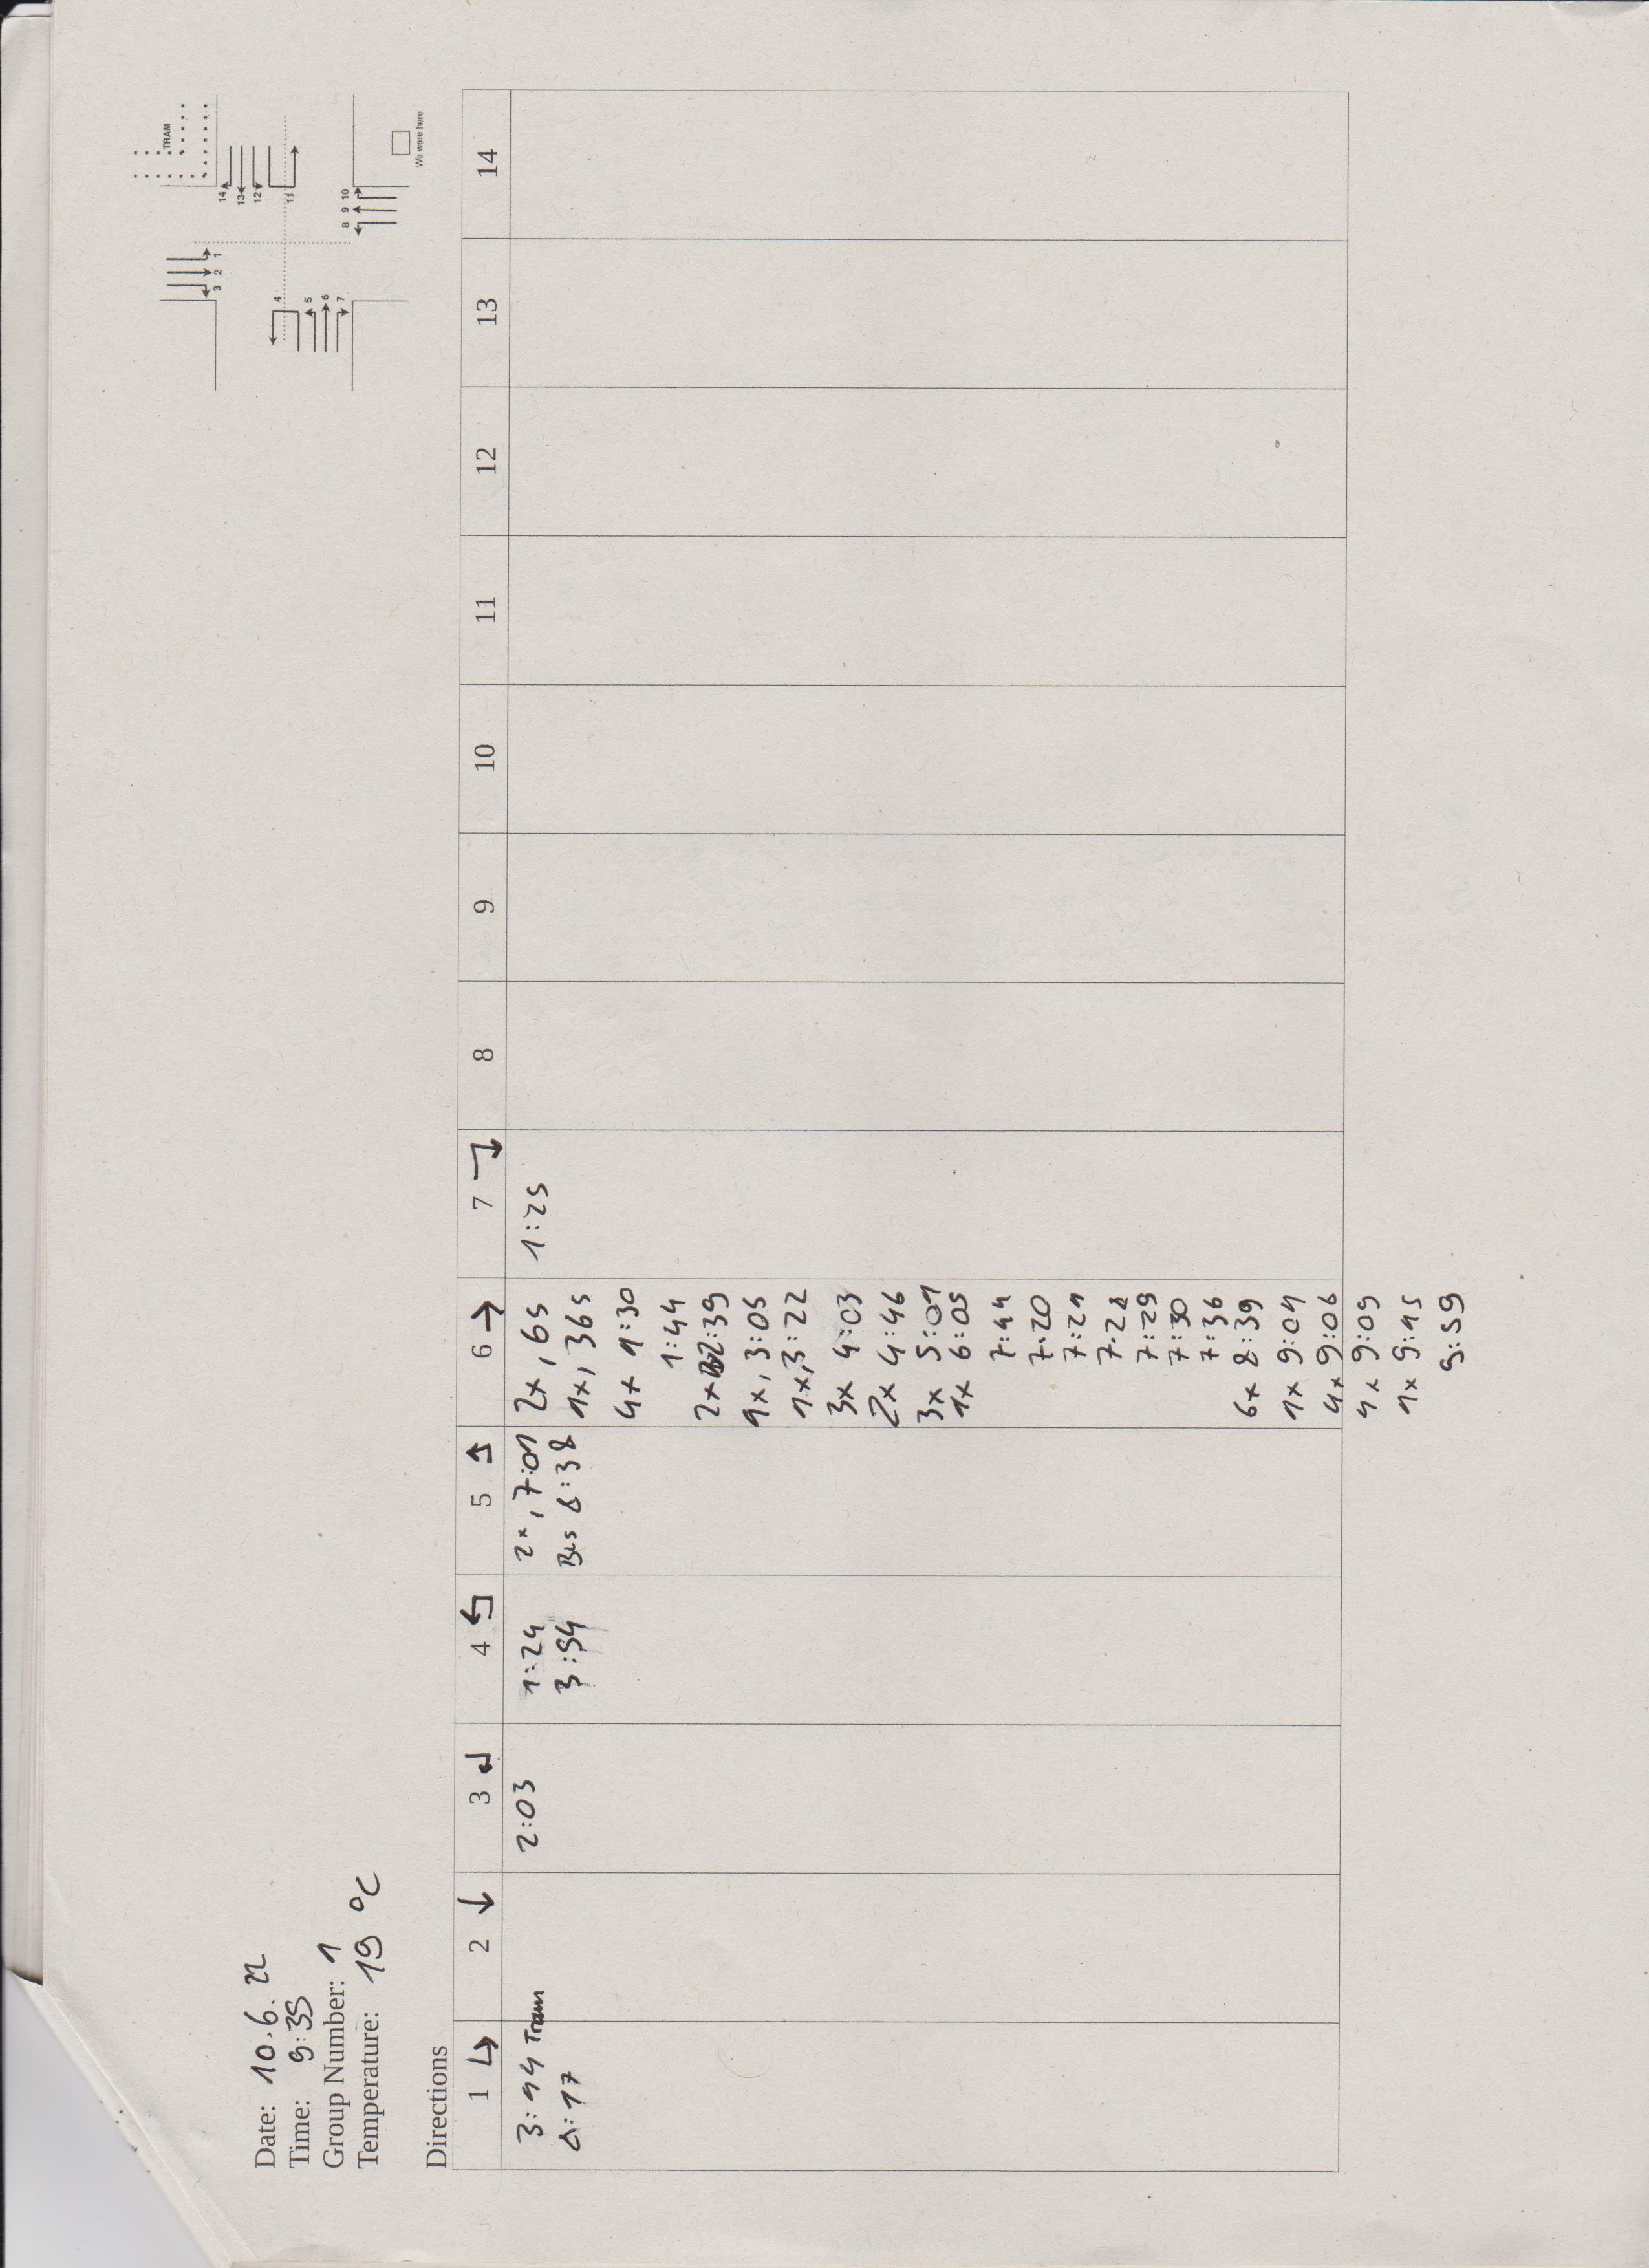
\includegraphics[width=\linewidth]{scans/Bild (15).jpg}
\end{figure*}

\begin{figure*}[htbp]
  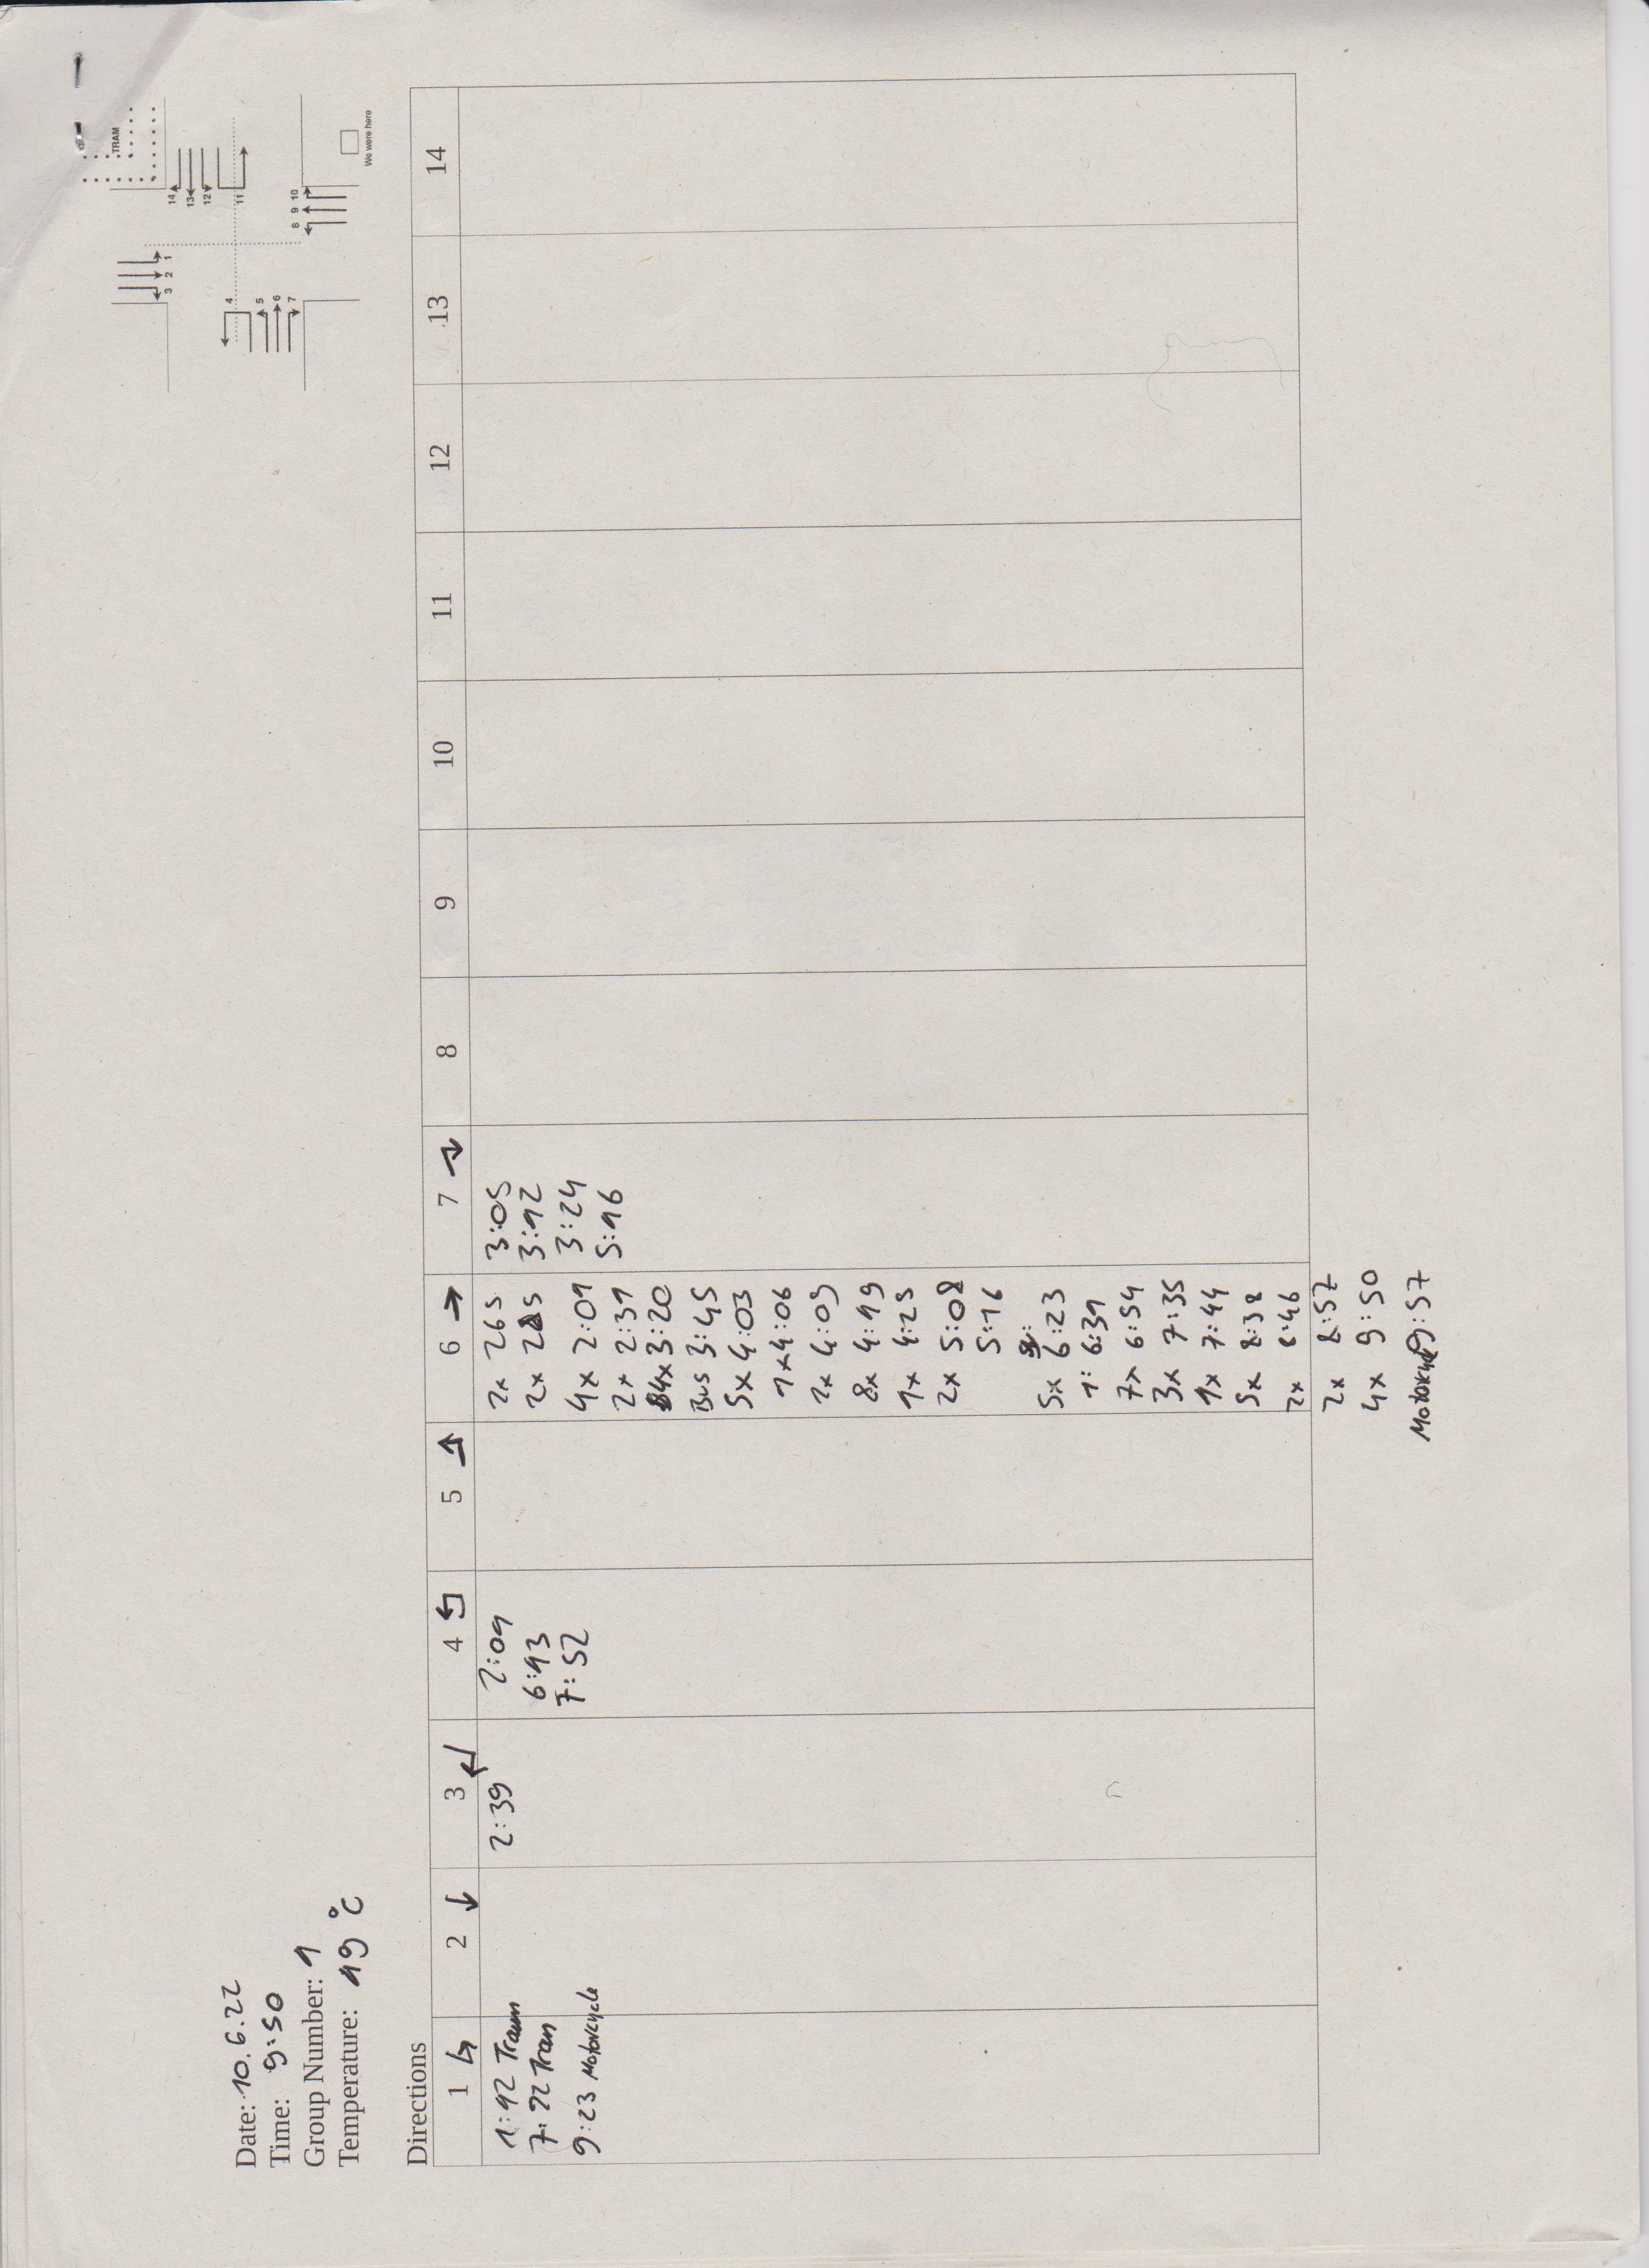
\includegraphics[width=\linewidth]{scans/Bild (16).jpg}
\end{figure*}

%\rotatebox{270}{\scalebox{.25}{\includegraphics[]{scans/Bild (1).jpg}}}\\\\
%\rotatebox{270}{\scalebox{.25}{\includegraphics[]{scans/Bild (2).jpg}}}\\\\
%\rotatebox{270}{\scalebox{.25}{\includegraphics[]{scans/Bild (3).jpg}}}\\\\
%\rotatebox{270}{\scalebox{.25}{\includegraphics[]{scans/Bild (4).jpg}}}\\\\
%\rotatebox{270}{\scalebox{.25}{\includegraphics[]{scans/Bild (5).jpg}}}\\\\
%\rotatebox{270}{\scalebox{.25}{\includegraphics[]{scans/Bild (6).jpg}}}\\\\
%\rotatebox{270}{\scalebox{.25}{\includegraphics[]{scans/Bild (7).jpg}}}\\\\
%\rotatebox{270}{\scalebox{.25}{\includegraphics[]{scans/Bild (8).jpg}}}\\\\
%\rotatebox{270}{\scalebox{.25}{\includegraphics[]{scans/Bild (9).jpg}}}\\\\
%\rotatebox{270}{\scalebox{.25}{\includegraphics[]{scans/Bild (10).jpg}}}\\\\
%\rotatebox{270}{\scalebox{.25}{\includegraphics[]{scans/Bild (11).jpg}}}\\\\
%\rotatebox{270}{\scalebox{.25}{\includegraphics[]{scans/Bild (12).jpg}}}\\\\
%\rotatebox{270}{\scalebox{.25}{\includegraphics[]{scans/Bild (13).jpg}}}\\\\
%\rotatebox{270}{\scalebox{.25}{\includegraphics[]{scans/Bild (14).jpg}}}\\\\
%\rotatebox{270}{\scalebox{.25}{\includegraphics[]{scans/Bild (15).jpg}}}\\\\
%\rotatebox{270}{\scalebox{.25}{\includegraphics[]{scans/Bild (16).jpg}}}

 \section{Conclusion}
During these four vehicular experiments, data from over 2300 vehicles was collected at the intersection at the University of Bremen, Germany, of which 95.53\% were private vehicles. Through the expansion of the overall data set, this data can be used in future works, such as training mobility models or vehicular traffic research. With that, the aim of providing real-world data on traffic was successfully achieved. \newpage



\bibliographystyle{abbrv}
\bibliography{sigproc}
%\newpage
\section{Appendix}
\subsection{Changes}
\begin{itemize}
    \item Changed former Background \& Summary to Introduction 
    \item Reworked and removed some parts of the text
    \item Added conclusion
    \item Added ''Bremen, Germany'' to Methods and intersection caption
    \item Moved date \& times from Technical Validation to Methods and added a table
    \item Increased size of intersection sketch 
    \item Improved axis scaling and labeling in Figure 4 
    \item Fixed spelling and grammar issues
    \item Thenuka indicated an error in the digitalization of our data, the data set was fixed and the data in the paper was adjusted accordingly
    \item Increased raw data sheet size in Appendix
    \item Uploaded the data to GitHub
    
\end{itemize}
\label{sec:Section 5}

\begin{figure*}[htbp]
  \includegraphics[width=\linewidth]{scans/300522_0805.pdf}
\end{figure*}

\begin{figure*}[htbp]
  \includegraphics[width=\linewidth]{scans/300522_0820.pdf}
\end{figure*}

\begin{figure*}[htbp]
  \includegraphics[width=\linewidth]{scans/300522_0835.pdf}
\end{figure*}

\begin{figure*}[htbp]
  \includegraphics[width=\linewidth]{scans/300522_0850.pdf}
\end{figure*}


%\rotatebox{270}{\scalebox{.25}{\includegraphics[]{scans/300522_0805.pdf}}}\\\\
%\rotatebox{270}{\scalebox{.25}{\includegraphics[]{scans/300522_0820.pdf}}}\\\\
%\rotatebox{90}{\scalebox{.25}{\includegraphics[]{scans/300522_0835.pdf}}}\\\\
%\rotatebox{270}{\scalebox{.25}{\includegraphics[]{scans/300522_0850.pdf}}}\\\\

\begin{figure*}[htbp]
  \includegraphics[width=\linewidth]{scans/300522_0905.pdf}
\end{figure*}

\begin{figure*}[htbp]
  \includegraphics[width=\linewidth]{scans/300522_0920.pdf}
\end{figure*}

\begin{figure*}[htbp]
  \includegraphics[width=\linewidth]{scans/300522_0935.pdf}
\end{figure*}

\begin{figure*}[htbp]
  \includegraphics[width=\linewidth]{scans/300522_0950.pdf}
\end{figure*}

%\rotatebox{270}{\scalebox{.25}{\includegraphics[]{scans/300522_0905.pdf}}}\\\\
%\rotatebox{270}{\scalebox{.25}{\includegraphics[]{scans/300522_0920.pdf}}}\\\\
%\rotatebox{270}{\scalebox{.25}{\includegraphics[]{scans/300522_0935.pdf}}}\\\\
%\rotatebox{270}{\scalebox{.25}{\includegraphics[]{scans/300522_0950.pdf}}}\\\\

\begin{figure*}[htbp]
  \includegraphics[width=\linewidth]{scans/030622_0905.pdf}
\end{figure*}

\begin{figure*}[htbp]
  \includegraphics[width=\linewidth]{scans/030622_0920.pdf}
\end{figure*}

\begin{figure*}[htbp]
  \includegraphics[width=\linewidth]{scans/030622_0935.pdf}
\end{figure*}

\begin{figure*}[htbp]
  \includegraphics[width=\linewidth]{scans/030622_0950.pdf}
\end{figure*}

%\rotatebox{270}{\scalebox{.25}{\includegraphics[]{scans/030622_0905.pdf}}}\\\\
%\rotatebox{270}{\scalebox{.25}{\includegraphics[]{scans/030622_0920.pdf}}}\\\\
%\rotatebox{270}{\scalebox{.25}{\includegraphics[]{scans/030622_0935.pdf}}}\\\\
%\rotatebox{270}{\scalebox{.25}{\includegraphics[]{scans/030622_0950.pdf}}}\\\\

\begin{figure*}[htbp]
  \includegraphics[width=\linewidth]{scans/100622_0905.pdf}
\end{figure*}

\begin{figure*}[htbp]
  \includegraphics[width=\linewidth]{scans/100622_0920.pdf}
\end{figure*}

\begin{figure*}[htbp]
  \includegraphics[width=\linewidth]{scans/100622_0935.pdf}
\end{figure*}

\begin{figure*}[htbp]
  \includegraphics[width=\linewidth]{scans/100622_0950.pdf}
\end{figure*}

%\rotatebox{270}{\scalebox{.25}{\includegraphics[]{scans/100622_0905.pdf}}}\\\\
%\rotatebox{270}{\scalebox{.25}{\includegraphics[]{scans/100622_0920.pdf}}}\\\\
%\rotatebox{270}{\scalebox{.25}{\includegraphics[]{scans/100622_0935.pdf}}}\\\\
%\rotatebox{270}{\scalebox{.25}{\includegraphics[]{scans/100622_0950.pdf}}}\\\\

\begin{figure*}[htbp]
  \includegraphics[width=\linewidth]{scans/Bild (1).jpg}
\end{figure*}

\begin{figure*}[htbp]
  \includegraphics[width=\linewidth]{scans/Bild (2).jpg})
\end{figure*}

\begin{figure*}[htbp]
  \includegraphics[width=\linewidth]{scans/Bild (3).jpg}
\end{figure*}

\begin{figure*}[htbp]
  \includegraphics[width=\linewidth]{scans/Bild (4).jpg}
\end{figure*}

\begin{figure*}[htbp]
  \includegraphics[width=\linewidth]{scans/Bild (5).jpg}
\end{figure*}

\begin{figure*}[htbp]
  \includegraphics[width=\linewidth]{scans/Bild (6).jpg}
\end{figure*}

\begin{figure*}[htbp]
  \includegraphics[width=\linewidth]{scans/Bild (7).jpg}
\end{figure*}

\begin{figure*}[htbp]
  \includegraphics[width=\linewidth]{scans/Bild (8).jpg}
\end{figure*}

\begin{figure*}[htbp]
  \includegraphics[width=\linewidth]{scans/Bild (9).jpg}
\end{figure*}

\begin{figure*}[htbp]
  \includegraphics[width=\linewidth]{scans/Bild (10).jpg}
\end{figure*}

\begin{figure*}[htbp]
  \includegraphics[width=\linewidth]{scans/Bild (11).jpg}
\end{figure*}

\begin{figure*}[htbp]
  \includegraphics[width=\linewidth]{scans/Bild (12).jpg}
\end{figure*}

\begin{figure*}[htbp]
  \includegraphics[width=\linewidth]{scans/Bild (13).jpg}
\end{figure*}

\begin{figure*}[htbp]
  \includegraphics[width=\linewidth]{scans/Bild (14).jpg}
\end{figure*}

\begin{figure*}[htbp]
  \includegraphics[width=\linewidth]{scans/Bild (15).jpg}
\end{figure*}

\begin{figure*}[htbp]
  \includegraphics[width=\linewidth]{scans/Bild (16).jpg}
\end{figure*}

%\rotatebox{270}{\scalebox{.25}{\includegraphics[]{scans/Bild (1).jpg}}}\\\\
%\rotatebox{270}{\scalebox{.25}{\includegraphics[]{scans/Bild (2).jpg}}}\\\\
%\rotatebox{270}{\scalebox{.25}{\includegraphics[]{scans/Bild (3).jpg}}}\\\\
%\rotatebox{270}{\scalebox{.25}{\includegraphics[]{scans/Bild (4).jpg}}}\\\\
%\rotatebox{270}{\scalebox{.25}{\includegraphics[]{scans/Bild (5).jpg}}}\\\\
%\rotatebox{270}{\scalebox{.25}{\includegraphics[]{scans/Bild (6).jpg}}}\\\\
%\rotatebox{270}{\scalebox{.25}{\includegraphics[]{scans/Bild (7).jpg}}}\\\\
%\rotatebox{270}{\scalebox{.25}{\includegraphics[]{scans/Bild (8).jpg}}}\\\\
%\rotatebox{270}{\scalebox{.25}{\includegraphics[]{scans/Bild (9).jpg}}}\\\\
%\rotatebox{270}{\scalebox{.25}{\includegraphics[]{scans/Bild (10).jpg}}}\\\\
%\rotatebox{270}{\scalebox{.25}{\includegraphics[]{scans/Bild (11).jpg}}}\\\\
%\rotatebox{270}{\scalebox{.25}{\includegraphics[]{scans/Bild (12).jpg}}}\\\\
%\rotatebox{270}{\scalebox{.25}{\includegraphics[]{scans/Bild (13).jpg}}}\\\\
%\rotatebox{270}{\scalebox{.25}{\includegraphics[]{scans/Bild (14).jpg}}}\\\\
%\rotatebox{270}{\scalebox{.25}{\includegraphics[]{scans/Bild (15).jpg}}}\\\\
%\rotatebox{270}{\scalebox{.25}{\includegraphics[]{scans/Bild (16).jpg}}}




\end{document}
